\chapter{In silico musculoskeletal model muscle personalization}
\label{chapter:4}

\usection{Introduction}
In human-robot interaction scenarios involving physical contact, knowledge of human force exertion limits is crucial for safe and effective collaboration. These limits can be represented by force feasible sets, which encapsulate all achievable hand forces given a specific posture and individual musculoskeletal properties.  Numerical simulation via musculoskeletal models enables the characterization of these sets, accounting for muscle architecture and neural control (\cite{skuricOnLineFeasibleWrench2022}; \cite{rezzougUpperLimbIsometricForce2021b}).

The shape of force feasible sets is primarily influenced by muscular neural control, which dictates the relative activation levels of different muscles. Chapter \ref{chapter:3} established an ellipsoidal approximation for these sets due to the high number of upper limb muscles, but did not provide information on their size or elongation for different muscle architectures. To address this gap, this chapter examines how muscle force-generating and geometric properties influence the size and elongation characteristics of force feasible sets across different postures.

Employing an \emph{in silico} approach, we utilize the Stanford upper limb musculoskeletal model (\cite{holzbaurModelUpperExtremity2005}) to simulate an individual's upper limb. This model incorporates a kinematic chain for the skeletal structure (bones and joints), with muscles defined as segments and curves attached to the skeleton. Muscle force generation is determined by a Hill-type model. With this model as a foundation, the chapter aims to extract the muscle geometry and their feasible forces from force feasible sets generated at the hand. Formulated as an optimization problem over multiple postures, this involves identifying Hill-type muscle functions and the muscle geometry in order to yield given force feasible sets.

Due to the geometric complexity of analyzing maximal force exertion sets, this chapter is structured as follows: section \ref{sec:musculoskeletal_model_muscle_pers_sec} introduces Stanford's upper limb musculoskeletal model and details the optimization problem formulation, including the challenge of comparing force feasible sets based on their shapes. It also discusses the computational difficulties and introduces suitable solvers. Section \ref{sec:personalization_silico_polytopes} utilizes these tools to investigate in an independent manner the retrieval of muscle geometric parameters and force-generating parameters under a $\mathcal{T}_{\infty}$ muscle activation model, resulting in polytopic force feasible sets. While insightful, this approach reveals computational limitations. Section \ref{sec:personalization_silico_ellipsoid} addresses these limitations by incorporating the force feasible set ellipsoidal approximation from chapter \ref{chapter:3} into the optimization process. This section takes advantage of the biomechanical interpretation of force feasible sets as ellipsoids, significantly improving the feasibility of the personalization.

The chapter concludes in \ref{sec:chapter_4_conclusion} with a discussion on the in silico approach and personalization quality, leading into chapter \ref{chapter:5}, which focuses on personalizing the Stanford model using experimentally measured maximal force exertions in three postures.

\section{Musculoskeletal model muscle personalization based on force feasible sets}
\label{sec:musculoskeletal_model_muscle_pers_sec}

As one of our goals is to extend muscle personalization from in silico force feasible sets to experimentally measured force exertion, a numerical human representation, namely a \emph{musculoskeletal model}, is required. Building upon its skeletal and muscle description in \ref{subsec:generic_msk}, the personalization process as an optimization problem is formulated in \ref{subsec:optimization_pb}. While the problem is posed theoretically for convenience, subsection \ref{subsec:comparing_ffs} delves into the practical issues of defining a notion of similarity between 3D shapes, which is necessarily required in our optimization framework. Additionally, specific solvers are thoroughly described in \ref{subsec:non_differentiability} to handle the high-dimensionality of the muscle parameters search space and the non-differentiability of our cost function. This section ends in \ref{subsec:validation_optimization_pb} on the \emph{quality} of a found solution, in terms of reproduced force feasible sets in specific postures but also in other postures. The methods outlined in this section provide a framework for developing and implementing the optimization process across a range of scenarios (involving different force feasible set representations, distances between sets, specific search spaces, postures to optimize on, etc.) in the subsequent sections.

\subsection{Generic upper limb musculoskeletal model}
\label{subsec:generic_msk}
\begin{figure}[!htb]
    \centering
    \captionsetup{justification=centering}
    \begin{minipage}{1\linewidth}
        \captionsetup{justification=centering}
        \centering
        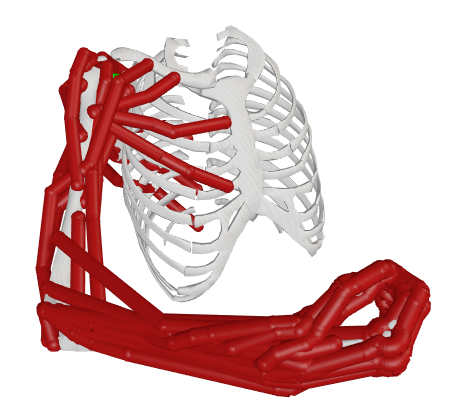
\includegraphics[trim={20 0 20 0}, clip, width=0.2\linewidth]{img/chapter_4/full_stanford.png}
    \end{minipage}
    \caption{Stanford's upper limb musculoskeletal model developped in (\cite{holzbaurModelUpperExtremity2005}). Visualization using OpenSim open-source software (\cite{delpOpenSimOpenSourceSoftware2007}).}
    \label{fig:stanford_full}
\end{figure}
\paragraph*{Stanford's upper limb model.} Stanford's right upper limb musculoskeletal model has been developped in (\cite{holzbaurModelUpperExtremity2005}). This model provides a detailed representation of the human upper extremity by including a thorough modelization of upper limb major muscles and joints.  The model is available online\footnote{\url{https://simtk.org/projects/up-ext-model}} as an XML file to import through the open-source musculoskeletal model software OpenSim\footnote{\url{https://simtk.org/projects/opensim}} (\cite{delpOpenSimOpenSourceSoftware2007}).

The model joint kinematics incorporates 15 degrees of freedom, allowing the simulation of a wide range of upper limb movements. The model encompasses the shoulder, elbow, forearm, wrist, but also the thumb and index finger motion. The motion between the scapula and humerus is defined through a ball-and-socket joint. The shoulder motion is defined as a combination of the clavicle, scapula and humerus motion depending on regression equations described in (\cite{degrootThreedimensionalRegressionModel2001}), in which the axes of rotations, degrees of freedom and order of rotations are defined and conform to the recommendations of the Internal Society of Biomechanics (\cite{wuISBRecommendationDefinitions2005}). The shoulder motion is adapted to depend only on the shoulder elevation angle. Concerning the elbow motion, it is modelized as two successive pivot rotations corresponding to the elbow flexion-extension motion and the forearm pronation-supination respectively. The first one corresponds to a rotation in the sagittal plane when the upper limb is in neutral position and its rotation angle varies from $0$° (full extension) to $130$° (flexion). The elbow pronation-supination rotation axis was determined numerically to ensure it passing through the center of the distal ulna, with angles varying between $90$° (pronation) to $-90$° (supination).
The wrist motion is also described as two successive rotations whose axes are described in (\cite{rubyRelativeMotionSelected1988}). The first motion corresponds to the wrist deviation ranging from $-10$° (radial) to $25$° (ulnar), then followed by the wrist flexion motion parametrized between $-70$° (extension) to $70$° (flexion). While we do not focus on the thumb and index finger motion, they have been modelized as rotations whose axis and center of rotations have also been defined in the literature.


Stanford's model includes also 50 individual muscles based on anatomical studies and physiological data. Each muscle is modeled with detailed origin and insertion attachment points with wrapping surfaces to account for their paths around bones and joints but also specificities of some muscles such as having multiple tendons, distinct heads or wide attachments. These attachment points are denoted as the \emph{geometric parameters} of a muscle. Force-generating properties of a muscle are modelized and based on a Hill-type muscle model. Namely, they corresponds to four parameters (optimal fiber length, maximal isometric force, tendon slack length and pennation angles), which have been gathered through anatomical studies. Both geometric and force-generating parameters allow for accurate simulation of muscle forces, moment arms, and their contribution to joint movements.

In order to validate the relevancy of this upper limb model as a simulation tool, Holzbaur et al. compared the biomechanical properties of their model to experimental data. Mainly, the model ensures an adequacy between in silico and in vivo maximum isometric joint moments. Muscle moment arms were also compared with experimental data, and while there are differences between measured and computed moment arm magnitude (mainly for shoulder muscles), the model does still agree with experimentally-measured isometric joint moments.

As such, Stanford's model is particularly well-suited to be used as a generic musculoskeletal upper limb model for force feasible set estimation. To numerically estimate the feasible tension range of each muscle, a muscle force model must be defined.
Numerous models have been developed to describe muscle tension based on the dynamic interactions between muscle fibers (\cite{zajacMuscleTendonProperties1989a}; \cite{thelenAdjustmentMuscleMechanics2003}; \cite{cadovaComparativeStudyMuscle2014}; \cite{millardFlexingComputationalMuscle2013a}). This chapter focuses on a widely used Hill-type muscle model, namely the Hill-Thelen muscle model.  While the Hill-Thelen model offers a comprehensive representation of muscle dynamics, the functional complexity of the model presents challenges in the context of muscle personalization.
To balance accuracy and complexity, we employ a simplified variant of this model, which will be described in the following paragraphs. This simplification allows for efficient representation of force generation under isometric conditions, while still capturing the essential complexities of muscle behavior and utilizing most of the model's muscle properties.

\paragraph*{The Hill-Thelen muscle model.} The Hill muscle model originates from Hill's work on muscle thermodynamical properties (\cite{hillHeatShorteningDynamic1938}; \cite{zajacMuscleTendonProperties1989a}). By considering the whole musculotendon structure as a mechanical actuator, 3 components are described: an active contractile element (CE) representing the force generated by the interaction of actin and myosin filaments; a passive elastic element (PE), represented as a spring in parallel with the CE, which accounts for the passive resistance of the muscle to stretch; and a serial elastic tendon (SE) modeled as a spring in series with the contractile element and accounting for the elastic properties of the tendon. 

Forces are produced by each of these three components. For a specific muscle $M$, the force in the contractile element has a non-linear relationship with muscle length, called the active-force-length relationship $f^L(\tilde{l}^M)$, where $\tilde{l}^M = l^M / l_o^M$ is the muscle length $l^M$ (in meters) normalized by the \emph{optimal fiber length} $l_o^M$ (in meters) at which $f^L$ peaks at $f_o^M$, the \emph{maximal isometric force} (in Newton). For non-isometric muscle contractions, the velocity of contraction $v^M$ (in m/s) also influences the force produced by the contractile element. This is the \emph{force-velocity} relationship, denoted as $f^V(\tilde{v}^M)$, where $\tilde{v}^M$ is the current velocity $v^M$ normalized by the velocity $v^M_{max}$ where $f^V$ reaches its peak. Under isometric conditions, where there is no contraction velocity, it is assumed that $f^V(\tilde{v}^M) = 1$. The CE also depends on a neural motor control, which dictates how much a muscle should be \emph{activated}. This is described by a scalar $a$ ranging from $0$ to $1$. As such, the CE produces tensions following the curve $af_o^Mf^L(\tilde{l}^M)f^V(\tilde{v}^M)$.

Both the passive elastic element (PE) and the serial elastic tendon (SE) are modeled as springs, with forces dependent on their respective stretches. The PE force depends on the muscle fiber length while the SE force on the tendon length. The PE force-length relationship, termed the \emph{passive force}, is a function of the normalized muscle fiber length $\tilde{l}^M$ and denoted by $f^{PE}(\tilde{l}^M)$. Conversely, the SE force-length relationship, termed the \emph{strain force}, is a function of $\tilde{l}^T$, the tendon length $l^T$ normalized by the tendon slack length $l_s^T$ (the length at which the tendon begins to generate force), and is denoted by $f^T(\tilde{l}^T)$.

% The PE force-length curve, called the \emph{passive force}, depends on the (normalized) muscle length $\tilde{l}^M$, and is denoted by $f^{PE}(\tilde{l}^M)$, whereas the SE force-length curve, called the \emph{strain force}, depends on $\tilde{l}^T$, the tendon length $l^T$ normalized by the \emph{tendon slack length} $l_s^T$ (the length at which the tendon begins to generate force), via a curve denoted $f^T(\tilde{l}^T)$.
\begin{figure}[!htb]
    \centering
    \captionsetup{justification=centering}
    \begin{minipage}{1\linewidth}
        \captionsetup{justification=centering}
        \centering
        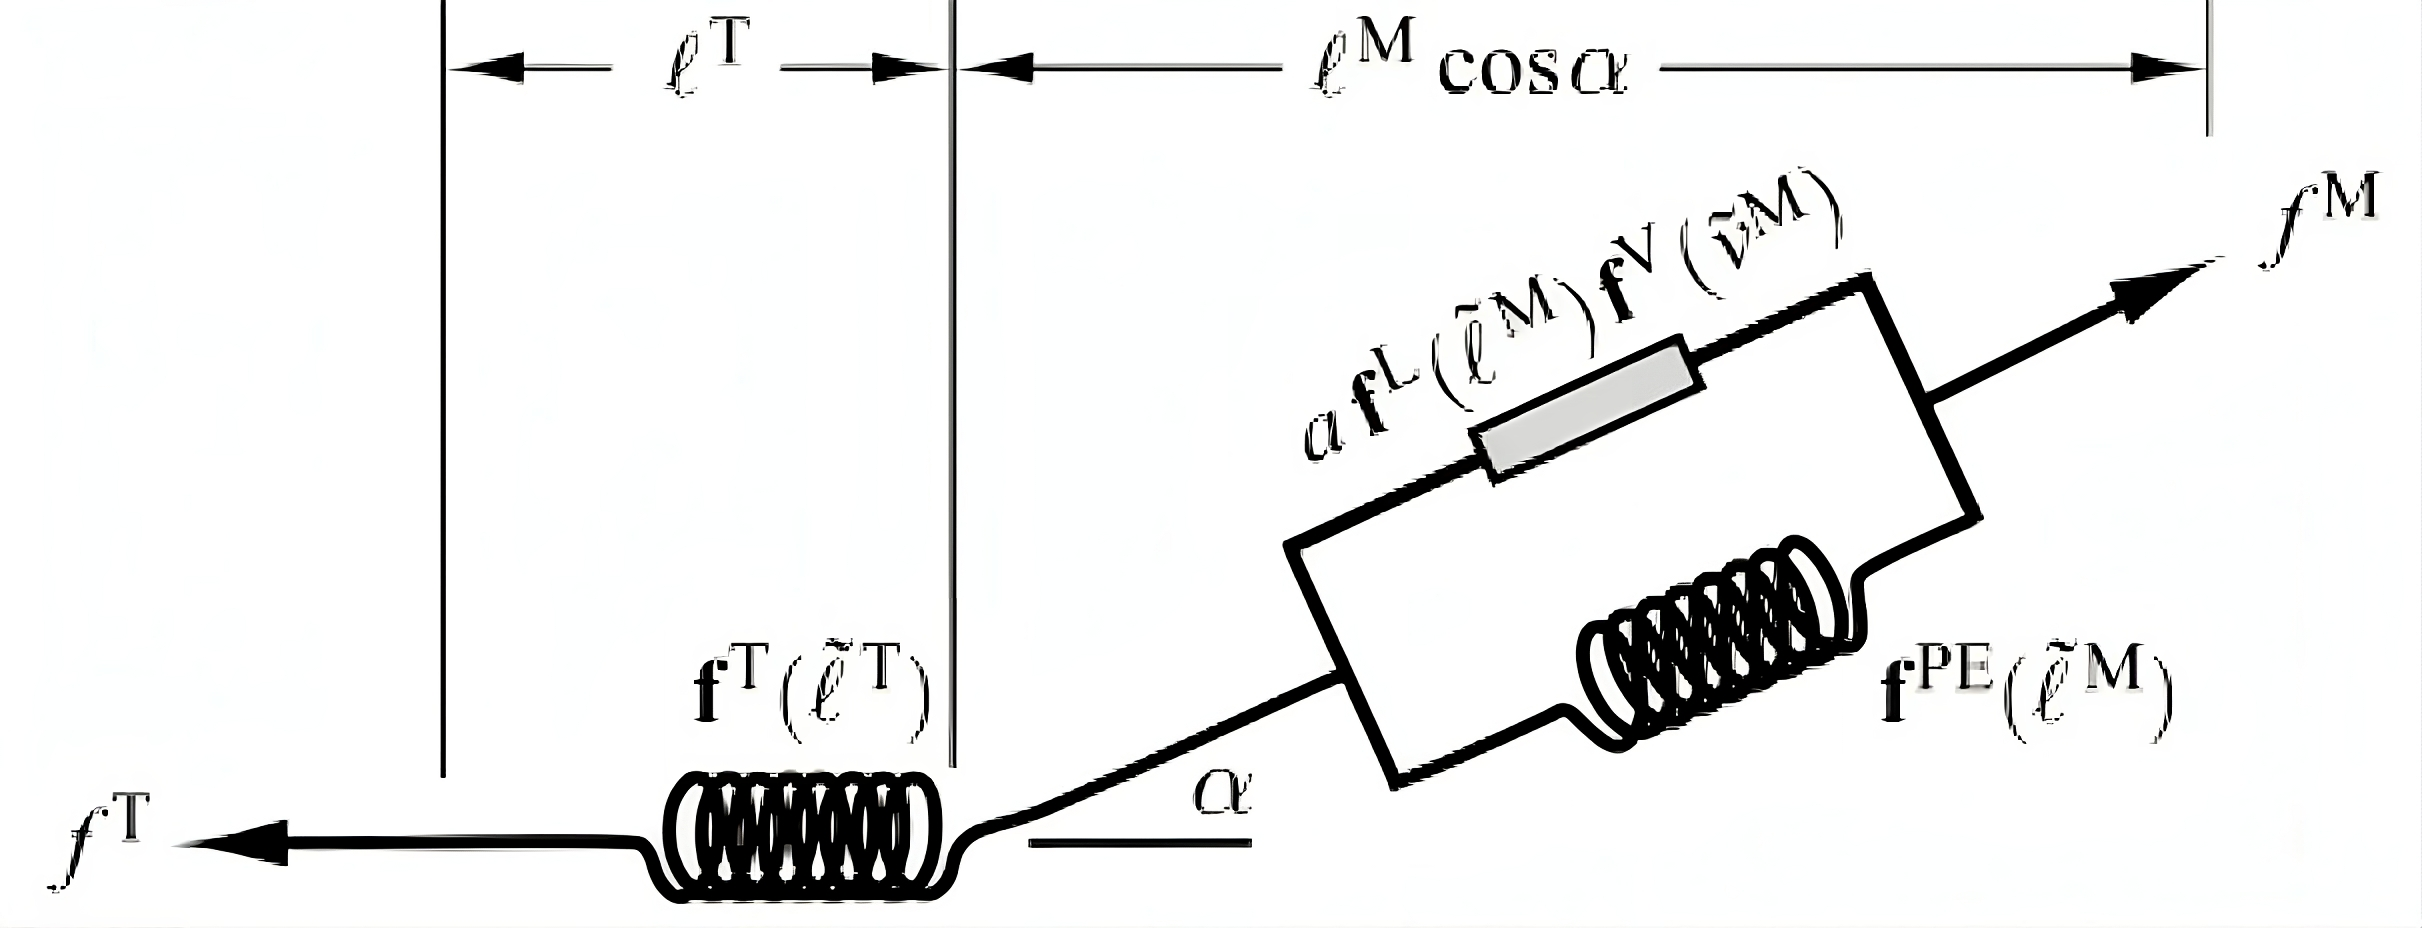
\includegraphics[trim={0 0 0 0}, clip, width=0.6\linewidth]{img/chapter_4/hill_model.png}
    \end{minipage}
    \caption{The Hill mechanical muscle model (figure extracted from (\cite{millardFlexingComputationalMuscle2013a})).}
    \label{fig:hil_model}
\end{figure}

Muscle fibers typically attach to tendons at an angle, termed the \emph{pennation angle} and denoted $\alpha$ (in radians). Accurate force representation necessitates accounting for this angle by multiplying the contractile and passive forces by $\cos(\alpha)$. However, in (\cite{holzbaurModelUpperExtremity2005}), a summary of pennation angles shows that most upper limb muscles exhibit small pennation, with the largest angle observed in the coracobrachialis muscle ($27$°), where $\cos(27$°$) \approx 0.89$. Given this minimal impact, pennation angle is not incorporated into the current model.

Thelen's muscle model yields explicit mathematical equations that describe the interplay between its constituent components. The following equations, as presented by Thelen in (\cite{thelenAdjustmentMuscleMechanics2003}), characterize these relationships. The force-length relationship of the contractile element $f^L(\tilde{l}^M)$ and the passive force $f^{PE}(\tilde{l}^M)$ are described as:
\begin{align*}
    f^L(\tilde{l}^M) &= e^{-(\tilde{l}^M -1)^2 / 0.45} \\
    f^{PE}(\tilde{l}^M) &= \frac{e^{5(\tilde{l}^M - 1) / \varepsilon} - 1}{e^5 - 1}
\end{align*}
where $\varepsilon$ is a parameter on an individual age. Thelen showed that age influences muscle mechanics, particularly tendon stiffness.
This age-related effect is modeled using parameter $\varepsilon > 0$, where $\varepsilon = 0.6$ represents young adults and $\varepsilon = 0.5$ represents older adults. As this chapter does not specifically investigate age-related effects, we set $\varepsilon = 0.5$, focusing on the young adult population.

Under isometric conditions, muscles are assumed to be in \emph{equilibrium}, implying that the force exerted by the muscle fibers compensates the force exerted by the tendon.
The force-generating properties of a muscle in Stanford's model are characterized by the \emph{maximal isometric force} $f_o^M$ (N), the \emph{optimal fiber length} $l_o^M$ (m) at which the muscle exerts its peak force, and the \emph{tendon slack length} $l_s^T$, which in our case corresponds to the length of the tendon (used to compute the muscle fiber length $l^M$ via the geometric relationship $l^M = l^{MT} - l_s^T$, where $l^{MT}$ is the musculotendon length derived from muscle path points).

The total muscle force $f^M$ is thus defined, in isometric condition, as
\begin{align*}
    f^M(a,\, l^{MT}, \, l_s^T,\, l_o^M,\,f_o^M) = f_o^M \cdot \left( af^L(\tilde{l}^M) + f^{PE}(\tilde{l}^M) \right)
\end{align*}
where $\tilde{l}^M = (l^{MT} - l_s^T) / l_o^M$. Thus, muscle force is a function of: (1) geometric parameters, represented by the muscle path length $l^{MT}$; (2) neural motor control (via muscle activation $a$); and (3) biomechanical muscle parameters, including maximal isometric force $f_o^M$, optimal fiber length $l_o^M$, and tendon slack length $l_s^T$.

Muscle length varies depending on the definition of its path points and a joint configuration of Stanford's model. As described, muscle force is a function of muscle length, implying that joint configuration influences the force-feasible sets. The following paragraphs focus on a specific joint configuration relevant to isometric conditions, namely, a \emph{static posture}, or simply \emph{posture}.

\paragraph*{Posture parametrization}
In Stanford's model, let us consider only the shoulder, elbow and wrist motions. These motions are parametrized by 7 generalized coordinates: 3 for the shoulder joint, 2 for the elbow and 2 for the wrist. We denote by $\mathbf{q} = (q_1, \dots, q_7)\in\IR^7$ the parametrization of these motions in their order of definition. $\mathbf{q}$ is called a \emph{posture} if $\ddot{\mathbf{q}} = 0$, $\dot{\mathbf{q}} = 0$ and all muscles are in equilibrium. 

For a posture $\mathbf{q}\in\IR^7$, since each generalized coordinate $q_i$ for $i = 1, \dots, 7$ is limited in range, we denote by $\mathcal{Q}$ the set of all possible postures such that $\mathbf{q}\in\mathcal{Q}$. 

\begin{figure}[!htb]
    \centering
    \captionsetup{justification=centering}
    \begin{minipage}{0.3\linewidth}
        \centering
        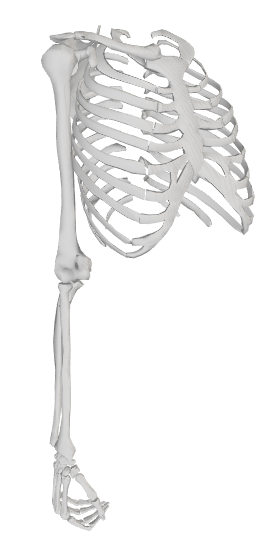
\includegraphics[trim={0 0 0 0}, clip, width=0.6\linewidth]{img/chapter_4/stanford_view.png}
    \end{minipage}
    \hfill
    \begin{minipage}{0.3\linewidth}
        \captionsetup{justification=centering}
        \centering
        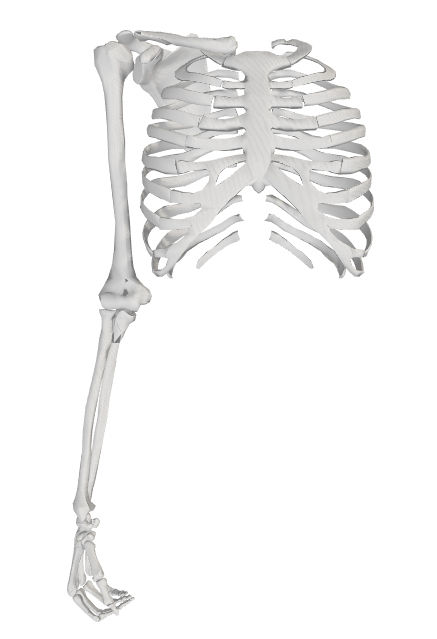
\includegraphics[trim={0 0 0 0}, clip, width=0.8\linewidth]{img/chapter_4/stanford_frontal_coronal.png}
    \end{minipage}
    \hfill
    \begin{minipage}{0.3\linewidth}
        \captionsetup{justification=centering}
        \centering
        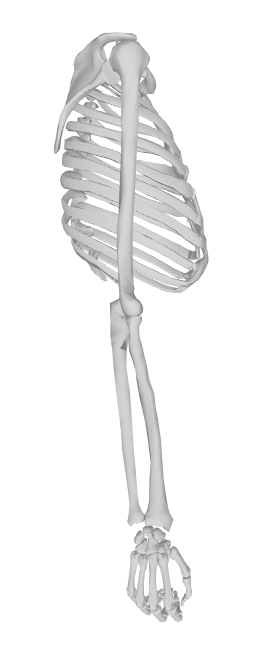
\includegraphics[trim={0 0 0 0}, clip, width=0.5\linewidth]{img/chapter_4/stanford_sagittal.png}
    \end{minipage}
    \caption{Visualization of Stanford's model in (neutral) posture $\mathbf{q} = (0, 0,0,0,0,0,0)$.}
    \label{fig:stanford_neutral_pose}
\end{figure}

\begin{figure}[!htb]
    \centering
    \captionsetup{justification=centering}
    \begin{minipage}{0.3\linewidth}
        \centering
        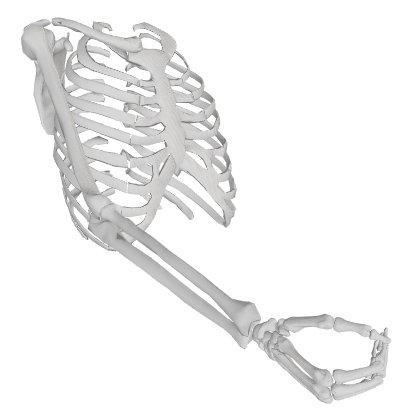
\includegraphics[trim={0 0 0 0}, clip, width=0.6\linewidth]{img/chapter_4/stanford_view_pose1.png}
    \end{minipage}
    \hfill
    \begin{minipage}{0.3\linewidth}
        \captionsetup{justification=centering}
        \centering
        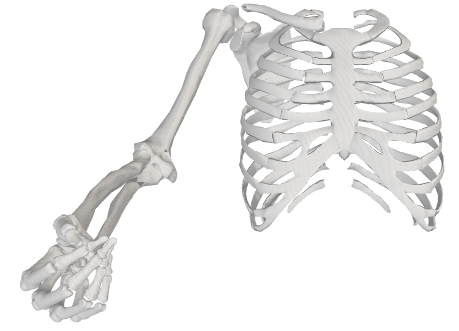
\includegraphics[trim={0 0 0 0}, clip, width=0.8\linewidth]{img/chapter_4/stanford_frontal_pose1.png}
    \end{minipage}
    \hfill
    \begin{minipage}{0.3\linewidth}
        \captionsetup{justification=centering}
        \centering
        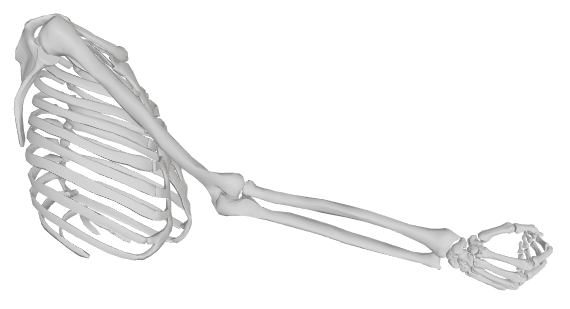
\includegraphics[trim={0 0 0 0}, clip, width=0.9\linewidth]{img/chapter_4/stanford_sagittal_pose1.png}
    \end{minipage}
    \caption{Visualization of Stanford's model in posture $\mathbf{q} = (70, 50, 40, 20, -70, 0, 0)$.}
    \label{fig:stanford_pose_1}
\end{figure}

Any posture influences the length of at least one muscle in Stanford's model.

\subsection{Muscle personalization through an optimization approach}
\label{subsec:optimization_pb}
One of this chapter's objective is to gauge, in silico, to which extent some of Stanford's muscles parameters (origin and insertion points, maximal isometric force, optimal fiber length and tendon slack length) can be retrieved from force feasible sets computed at the hand for various postures. Our approach is to consider an optimization problem, which in our case is assimilated to finding at a vector $\mathbf{x}$ encapsulating how Stanford's muscles are parametrized and minimizing a real-valued function $f$ terms the \emph{cost function} or \emph{objective function}. This function should evaluate to $0$ whenever the produced force feasible sets by a parametrization of Stanford's model coincide with the ones to obtain. If such a parametrization $\mathbf{x}$ is found, we can \emph{then} assess how it \emph{generalizes} \emph{i.e.} how this parametrization produces force feasible sets in other postures sufficiently similar to expected force feasible sets. One of the main difficulty is to first find such a parametrization. 

This subsection thoroughly describes the optimization problem, from the considered Stanford's model parameters involved to the explicit formulation of the function to minimize, considering all tension set models. First, we shall recall the force feasible set formulation.  

Consider a posture $\mathbf{q}\in\mathcal{Q}$ and the feasible tension set $\mathcal{T}(\mathbf{q})$ whose shape describes how muscles are activated in regard to other muscle activations (\emph{cf.} chapter \ref{chapter:3}) at posture $\mathbf{q}$. The force feasible set $\mathcal{F}_X^{\mathcal{T}}(\mathbf{q})$ at a point $X$ of the Stanford's model is expressed as
\begin{align*}
    \mathcal{F}^{\mathcal{T}}_X(\mathbf{q}) = \left\{ \mathbf{f}\in\IR^3 \mid J^T_X(\mathbf{q})\mathbf{f} = -L^T(\mathbf{q})\mathbf{t}(\mathbf{q}) - \mathbf{G}(\mathbf{q}),\quad\mathbf{t}(\mathbf{q})\in \mathcal{T}(\mathbf{q}) \right\}
\end{align*}
where $L^T(\mathbf{q})\in\IR^{7\times 50}$ denotes the transpose of the lever arm matrix, which maps muscle tensions $\mathbf{t}(\mathbf{q})$ to the torque space; $J_X^T(\mathbf{q})\in\IR^{7\times 3}$ is the transpose of the jacobian matrix of Stanford's kinematic chain at point $X$ expressed in the ground, which maps the forces at point $X$ to the torque space and $\mathbf{G}(\mathbf{q})\in\IR^7$ is the gravitational torque vector.

We assume a constant muscle activation pattern across all postures, \emph{i.e.} $\mathcal{T}(\mathbf{q}) = \mathcal{T}$ for any posture $\mathbf{q}$.
We employ a $\mathcal{T}_{\infty}$ model, implying that muscles act on joints independently from the others and resulting in force feasible sets shaped as convex polytopes. Based on the prior findings of chapter \ref{chapter:3}, these sets are approximable by ellipsoids when considering a large number of muscles. Section \ref{sec:personalization_silico_ellipsoid} will adapt the optimization process accordingly. While it could be interesting to focus also on other $\mathcal{T}_p$ models, for $p > 2$, in these cases we did not find a computational way to express the surface of force feasible sets. Sampling methods can be used but in our case (with 50 muscles) they require a large set of samples which do not necessarily project onto the force feasible set surface. Also, since the objective is to gauge if a solution can be found, we focus on only computable force feasible sets \emph{i.e.} using a $\mathcal{T}_{\infty}$ (force polytopes) or $\mathcal{T}_2$ (force ellipsoids) model.

The next paragraph expresses the muscular parameters of interest in Stanford's model \emph{i.e.} those impacting directly the lever arm matrix $L(\mathbf{q})$ and the produced tensions $\mathbf{t}(\mathbf{q})$.

\paragraph*{The parameter set and the search space.}
Focusing solely on the Stanford model's geometric and force-generating parameters, we assume known bone positions, orientations, lengths, joint centers, and rotation axes. Besides, while two individuals have different muscle path locations, it is assumed that the attachment points of a muscle can be described similarly over individuals. As an example, the supraspinatus muscle in Holzbaur et al. consists of path of points defined from the scapula (where is located its origin attachment point) to the humerus (for its insertion point), so that this path definition will be preserved throughout the optimization process.

The parameter set comprises two families: the \emph{force-generating} and the \emph{geometric} parameters. The first includes the maximum isometric force $f_o^M$, optimal fiber length $l_o^M$ and tendon slack length $l_s^T$ for each of the $50$ muscles, totaling $150$ parameters. Geometric parameters include origin and insertion points for each muscle ($6$ parameters per muscle), yielding $300$ geometric parameters. The optimization problem thus involves at least $450$ parameters.

Each parameter is defined on a specific interval. This set of all values parameters can take is called the \emph{search space} and noted $\mathcal{X}$. As previous, the search space is defined for geometric and force-generating parameters separately.
Geometric parameter ranges are confined to $\pm 0.5$ cm intervals around default values from Holzbaur et al. so that the search space corresponds geometrically to a cube of edge length $1$ centered at the origin and insertion points. Force-generating parameters have wider ranges depending on their type:  $f_o^M \pm 400$ N, $l_o^M \pm 0.1$ m and $l_s^T \pm 0.1$ m. These ranges ensure a very wide variety of possible parameters.

To explicitely express the search space $\mathcal{X}$, it is defined  following the order of definition of the muscles defined in Stanford's model. For geometric parameters, let $\mathbf{O}^i\in\IR^3$ and $\mathbf{I}^i\in\IR^3$ be the vector representation in their frame of definition of the origin and insertion point of muscle $i$ for $i = 1, \dots, 50$. Then, the geometric search space for muscle $i$, $\mathcal{X}_G^i \subset \IR^6$, is defined as
\begin{align*}
    \mathcal{X}_G^i = [\mathbf{O}^i - 0.5\cdot \mathbf{1},\, \mathbf{O}^i + 0.5\cdot \mathbf{1}] \times [\mathbf{I}^i - 0.5\cdot\mathbf{1},\, \mathbf{I}^i + 0.5\cdot\mathbf{1}]
\end{align*}
where $\mathbf{1} = (1,1,1)^T$.

By denoting $f_o^i$, $l_o^i$ and $l_s^i$ the maximal isometric force, optimal fiber length and tendon slack length default values of muscle $i$, then the force-generating search space for muscle $i$, $\mathcal{X}_F^i \subset \IR^3$, is defined as 
\begin{align*}
    \mathcal{X}_F^i = [f_o^i - 400,\, f_o^i + 400] \times [l_o^i - 0.1,\, l_o^i + 0.1] \times [l_s^i - 0.1,\, l_s^i + 0.1]
\end{align*}

The search space of muscle $i$, $\mathcal{X}^i \subset \IR^{9}$, corresponds to the concatenation of the force-generating and the geometric parameters and is denoted $\mathcal{X}^i = \mathcal{X}_F^i\times \mathcal{X}_G^i$. The total search space of the parameters $\mathcal{X}\in \IR^{450}$ is thus defined as
\begin{align*}
    \mathcal{X} = \mathcal{X}^1 \times \dots \times \mathcal{X}^{50}
\end{align*} 

\paragraph*{The optimization problem.}
A \emph{solution} is defined to be an element $\theta \in \mathcal{X}$. Our optimization formulation consists on finding a solution minimizing the dissimilarity between force feasible sets of reference in given postures and the force feasible sets produced by the solution in the same postures.

Consider a specific solution $\hat{\theta}\in\mathcal{X}$ and a set of postures $\mathbf{Q}$. Let $\hat{\mathcal{F}}_X^{\mathcal{T}}(\mathbf{q})$ be the force feasible set  at point $X$ produced by Standord's model parametrized by solution $\hat{\theta}$ at posture $\mathbf{q} \in \mathcal{Q}$ considering a $\mathcal{T}$-model of the muscles feasible tensions.

The optimization problem is described as finding a solution $\theta^*\in\mathcal{X}$ such that 
\begin{align}
    \label{eq:opt_prb}
    \theta^* = \argmin_{\theta \in \mathcal{X}} \max_{\mathbf{q}\in\mathcal{Q}} d(\hat{\mathcal{F}}_X^{\mathcal{T}}(\mathbf{q}),\, \mathcal{F}_X^{\mathcal{T}}(\mathbf{q}, \theta))
\end{align}
where $\mathcal{Q}$ is a predefined set of selected postures; $\mathcal{F}_X^{\mathcal{T}}(\mathbf{q},\, \theta)$ is the force feasible set produced by Stanford's model parametrized by solution $\theta$ at posture $\mathbf{q}\in\mathcal{Q}$ considering a $\mathcal{T}$-model of the tension set; and $d$ is a function defined as follows:
let $K^3$ be the set of closed bounded convex sets of $\IR^3$, then
$d\,\colon K^3\to \IR_{>0}$ is a function assessing the dissimilarity between two closed 3D convex shapes. $d$ is thus called the \emph{dissimilarity} function. It has the property that for all $A,\, B \in K^3$, then $d(A,\, B) = 0 \iff A = B$.

The posture set $\mathcal{Q}$, the dissimilarity function $d$ and the model of the tension set $\mathcal{T}$ are called \emph{hyperparameters}. Each of them parametrize the \emph{cost function}, which corresponds to the function to be minimized in the optimization \ref{eq:opt_prb}. The major interest of this chapter lies in finding a set of hyperparameters that ensures the convergence towards a solution. Section \ref{sec:personalization_silico_polytopes} considers a $\mathcal{T}_{\infty}$ model while section \ref{sec:personalization_silico_ellipsoid} considers the ellipsoidal approximation of a $\mathcal{T}_{\infty}$ model (using the projection constant $\lambda_2(\ell^{50})$ defined in chapter \ref{chapter:3}). This second case also encapsulates the $\mathcal{T}_2$ tension models as well. In each of the sections, multiple dissimilarity functions are considered to account for the various representations of force feasible sets (as polytopes or ellipsoids) but also for the inherent difficulties related to the combinatorial vertex enumeration problem for polytopes (as described in chapter \ref{chapter:2}). While there are already existing dissimilarity functions between shapes, most of them are \emph{exact} and strongly fail to be relevant when using approximations of polytopes surfaces (for instance using Skuric et al's Iterative Convex Hull algorithm (\cite{skuricOnLineFeasibleWrench2022})). However, not using approximations in infeasible due to the high combinatorics inherent to polytopes. The next subsection dives in the required computational trade-offs in much depth.

Concerning the optimization formulation as a single-objective optimization (only one function is to be minimized), it could have been described as a multi-objective optimization (MOO) in which force feasible sets are compared in one posture only and independently from another posture. We chose to encapsulate the formulation into one cost function due to the computational challenges introduced by MOO as the required higher dimensionality of the search space, the higher number of solutions to evaluate and the higher number of iterations to ensure convergence (\cite{huaSurveyEvolutionaryAlgorithms2021}; \cite{okabeCriticalSurveyPerformance2003}).

Major issues arise in formulating the optimization problem. For instance, how many postures are required? Which dissimilarity function leads to the most relevant solution? Also, in a more fundamental way, which $\mathcal{Q}$ and $d$ allows us to converge to a solution? We will see in section \ref{sec:personalization_silico_ellipsoid} that it is possible to find a solution using the ellipsoidal approximation of a $\mathcal{T}_{\infty}$ model of the tension set.

Before diving into comparing force feasible sets, it must be noted that in the formulation \ref{eq:opt_prb}, it is still an open question to assess if $\hat{\theta} = \theta^*$ for some postures $\mathcal{Q}$. In other words, we do not know if two parametrizations of Stanford's model lead to the same force feasible sets. This could be proven (or not) by studying the injectivity of the cost function for the given postures $\mathcal{Q}$: due to the geometric nature of the force feasible sets (projection-intersection of sets), we did not suceed in achieving such a proof. 
However, we did find some answer in a more specific case: in cable-driven parallel robots such that any motion is either spherical or a 3 DOFs prismatic joint and cables are modelled as line segments, the produced torque feasible sets under a $\mathcal{T}_{\infty}$ model in only 3 postures uniquely define the line of action of each cable. These results are too specific to torque feasible sets and not force feasible sets, so we do not include them in this thesis.

% \paragraph*{Cost functions on sets}

\subsection{Comparing force feasible sets}
\label{subsec:comparing_ffs}
A major inconvenience in the optimization problem \ref{eq:opt_prb} is the nature of force feasible sets: they are \emph{convex sets}. While there are multiple ways to compare how two points (via euclidean distance), two vectors (via euclidean distance as well), two rotations (via geodesic), two $n$-dimensional spaces (via principal angles), or even two spatial vectors (via euclidean distance on both direction and moment part) are resembling each other, the force feasible sets nature implies a stronger difficulty in the comparison. The main difference from the above-mentionned objects is the existence of a non-null full-dimensional volume measure: essentially, a 3-dimensional convex set \emph{takes some space} in $\IR^3$ (whereas a line or a plane do not - and in a less tangible manner, rotations and translations do not either\footnote{A more tangible representation would be to consider rotations and translations as planes of a 5-dimensional Minkowski algebra, which is a specific structure based on a 5-dimensional real vector space (\cite{dorstGeometricAlgebraComputer2007}).}). Volume-related notions add another layer of computational complexity, whether or not the volume is explicitely computed. For instance, computing the volume of a polytope knowing its vertices and/or its bounding hyperplanes is a \#P-hard problem (\cite{dyerComplexityComputingVolume1988}): this class of problems involve counting the number of solutions to an NP-problem. In other terms, using the explicit notion of volume adds computational time to the already time-consuming step of computing the vertices (approximated or not) of a polytope.

The next paragraphs enunciate different methods to compare two convex sets, with a focus on leveraging expensive computational volume problems while retaining most of the required characteristics of force feasible sets to ensure an effective comparison.

\paragraph*{The Hausdorff distance between compact sets.}
The Hausdorff distance (\cite{hausdorffGrundzuegeMengenlehre1914}) is a measure of dissimilarity between two sets of points. It quantifies how far apart two shapes are from each other. In $\IR^n$, for $n \geq 1$, its definition is restricted to \emph{compact} sets, which are the closed and bounded sets (as are assumed the force feasible sets). We assume $\IR^n$ to be a metric space \emph{i.e.} it is equipped with a distance function, denoted $\delta$. 

The \emph{directed Hausdorff distance} between two compact sets $A$ and $B$, noted $\overrightarrow{d_H}(A,B)$, is defined as follows:
\begin{align*}
    \overrightarrow{d_H}(A,B) = \sup_{a\in A} \delta(a, B) = \sup_{a\in A} \inf_{b\in B} \delta(a, b)
\end{align*}

This directed distance captures the largest extent to which the set $B$ lies outside $A$. It is not a \emph{distance} in the mathematical sense as it is not symmetric, but it is usually called as such. The \emph{Hausdorff distance} introduces this symmetry and is noted $d_H$. It generalizes the directed distance concept by considering how much $A$ lies outside $B$ but also how much $B$ lies outside of $A$. In essence, it highlights the most significant mismatch between the two sets.
\begin{align*}
    d_H(A, B) = \max \left\{ \overrightarrow{d_H}(A,B),\, \overrightarrow{d_H}(B,A) \right\}
\end{align*}
The Hausdorff distance is a properly defined distance. Figure \ref{fig:hausdorff_distance_explained} shows how the Hausdorff distance is computed using generic shapes in 2D.

\begin{figure}[!htb]
    \captionsetup{justification=centering}
        \centering
        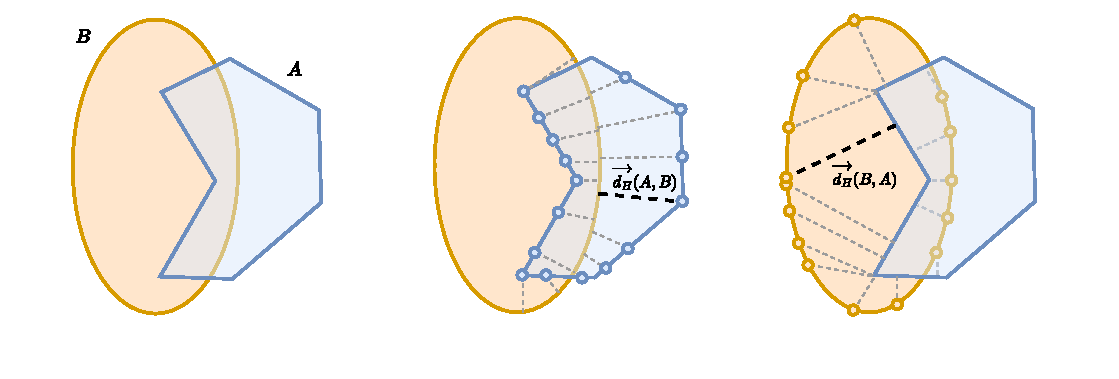
\includegraphics[trim={30 30 30 5},clip,width=0.9\linewidth]{img/chapter_4/hausdorff_distance_explained.pdf}
    \caption{The Hausdorff distance between sets $A$ (in blue) and $B$ (in orange) is computed as the maximum of the directed Hausdorff distances $\overrightarrow{d_H}(A,B)$ and $\overrightarrow{d_H}(B, A)$. The middle figure shows roughly how $\overrightarrow{d_H}(A,B)$ is computed: consider points on the surface of $A$ and find their closest points located on the surface of $B$. Compute all distances between these pairs of points and consider the greatest distance to be $\overrightarrow{d_H}(A,B)$ (in black). To compute $\overrightarrow{d_H}(B,A)$, the same process is applied starting from $B$'s surface (right figure).}
    \label{fig:hausdorff_distance_explained}
\end{figure}

Having a notion of distance on compact sets implies that a \emph{topology} can be defined onto compact sets \emph{i.e.} notions of convergence and limits are definable and consequently notions of approximations are as well. Hausdorff distance is explicitely computable for two polytopes, as are two force feasible sets modelled from a $\mathcal{T}_{\infty}$ tension set model. In this case, it is required to enumerate all polytopes vertices to compute it.

\paragraph*{Leveraging vertex count in force polytopes.} When comparing two force feasible sets $\mathcal{F}_1$ and $\mathcal{F}_2$ using a $\mathcal{T}_{\infty}$ tension model, the Hausdorff distance is relevant as long as $\mathcal{F}_1$ and $\mathcal{F}_2$'s vertices are computed using an \emph{exact} vertex enumeration algorithm. While the Hausdorff distance computation is of polynomial time when polytopes are in vertex representation (\emph{cf.} (\cite{konigComputationalAspectsHausdorff2014}) theorem 3.3), there remains to consider to computational aspect of gathering these vertices. Using Stanford's model, this implies to: (1) compute for some posture the $\mathcal{H}$-representation (bounding hyperplanes) of the projection of a $50$-dimensional orthotope onto the $7$-dimensional torque space; (2) find the smallest convex set encapsulated by these hyperplanes intersected with the image of the jacobian transpose; (3) then extract the vertices from the newly found set of bounding hyperplanes. Chapter \ref{chapter:2} recalls that step (1) is combinatorially very expensive; step (2) can be computed using the Fourier-Motzkin elimination method which has an exponential time complexity depending on the considered dimension (\cite{dahlCombinatorialPropertiesFourierMotzkin2007}) and step (3) is also combinatorially expensive as found by Avis in Fukuda in (\cite{avisPivotingAlgorithmConvex}). 

As such, an approximation of $\mathcal{F}_1$ and $\mathcal{F}_2$'s surface is required to ensure the evaluation of \emph{one} solution in the optimization problem in reasonnable time ($<1$ minute). We shall consider Skuric et al's \emph{Iterative Convex Hull} (ICH) method (\cite{skuricOnLineFeasibleWrench2022}), which returns a set of points located on the surface of a polytope formulated as a projection-then-intersection. ICH's implementation is available in Python 3 and MatLab (\cite{skuricPycapacityRealtimeTaskspace2023}).

However, Hausdorff distance is sentitive to the vertices locations, even when the global shapes are roughly similar. Figure \ref{fig:hausdorff_sensitivity} shows and describes the problem.
\begin{figure}[!htb]
    \captionsetup{justification=centering}
        \centering
        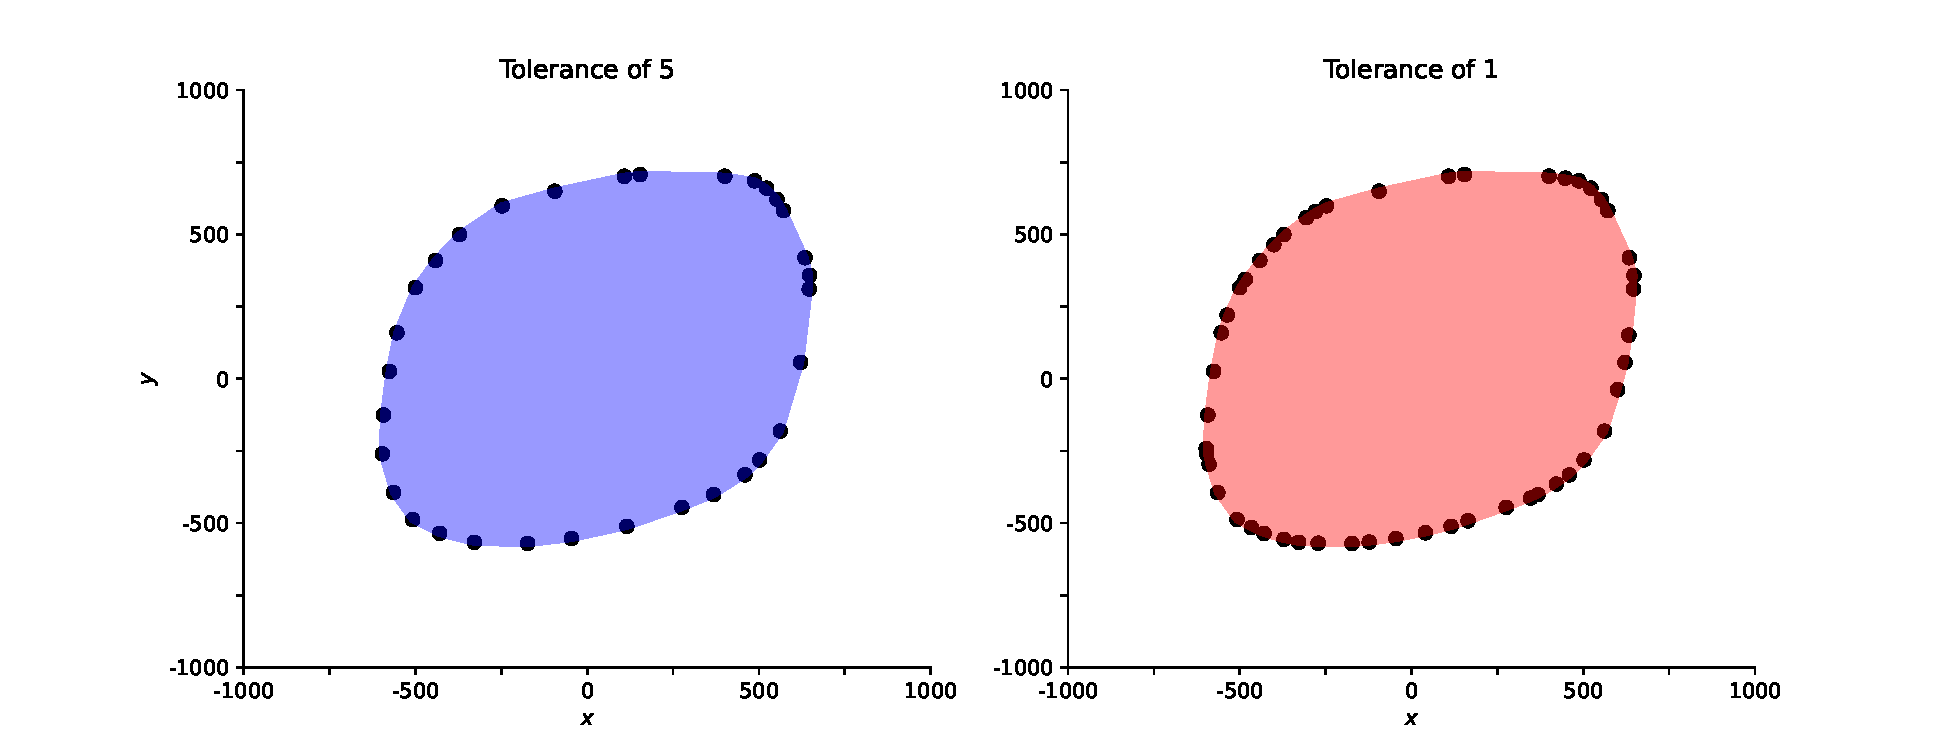
\includegraphics[trim={70 20 70 20},clip,width=1\linewidth]{img/chapter_4/chapter_4_hausdorff_sensitivity_1.pdf}
    \caption{Computation of a 2D polytope (polygon) considering a random projection onto a $7$-dimensional space of a random $50$-dimensional orthotope (edge lengths up to 800) intersected with a random $2$-dimensional vector space. The left polytope is computed with Skuric et al's ICH algorithm using a tolerance of $5$ while the right polytope uses a tolerance of $1$. This implies that the right polytope have much more vertices on its surface returned by ICH. The Hausdorff distance between these two shapes considers the euclidean distance between the polytopes vertices and is of value $97.17$. While the shapes are similar, this distance value is very far from $0$ and results from the high sensitivity of Hausdorff distance to vertices locations.}
    \label{fig:hausdorff_sensitivity}
\end{figure}

For our optimization problem, Hausdorff distance's sensitivity is an issue because of the force feasible sets as polytopes are approximated. To counteract this effect\footnote{There exists also the \emph{modified Hausdorff distance} (MHD), which is performant in the presence of noise (\cite{dubuissonModifiedHausdorffDistance1994}). However, MHD is more effective when \emph{only} the shapes are similar: two similar shapes with different scales have a low MHD value, which is not our objective as both shape and size matter in force feasible sets.}, we \emph{discretize} polytopes according to a family of vectors. The discretization process consists on intersecting a given polytope with a line and consider the intersection points. Using Stanford's model, a force feasible set computed at point $X$ at posture $\mathbf{q}$ has the point $X$ in its interior, so that a set of directions located at $X$ can be defined. Each of these lines intersect the force feasible set surface in $2$ points. 
The selection of these lines is drawn from the cube face lattice (\emph{i.e.} the structure of all it $k$-dimensional faces, $k=0, \dots, 2$, so its vertices, edges and faces). 
The cube, centered at the origin, has $8$ vertices. The first lines to construct are made from pairs of two symmetric vertices (the symmetry is central). This leads to $4$ lines. Then, edges are considered: there are 12 in the cube and each edge is centrally symmetric to another so that a line is defined to pass through an edge center and the symmetric edge center. This adds $6$ new lines. Finally, the $6$ cube faces, seen as squares, we consider for each of them the barycenter point constructed from their delimiting vertices (\emph{i.e.} the square center). Since central symmetry applies as well, $3$ new lines are defined and each of them pass through a face center and the corresponding other symmetric face center. In total, this leads to $13$ lines. Figure \ref{fig:polytope_discretization} summarizes these 13 line constructions.

\begin{figure}[!htb]
    \centering
    \captionsetup{justification=centering}
    \begin{minipage}{\linewidth}
        \centering
        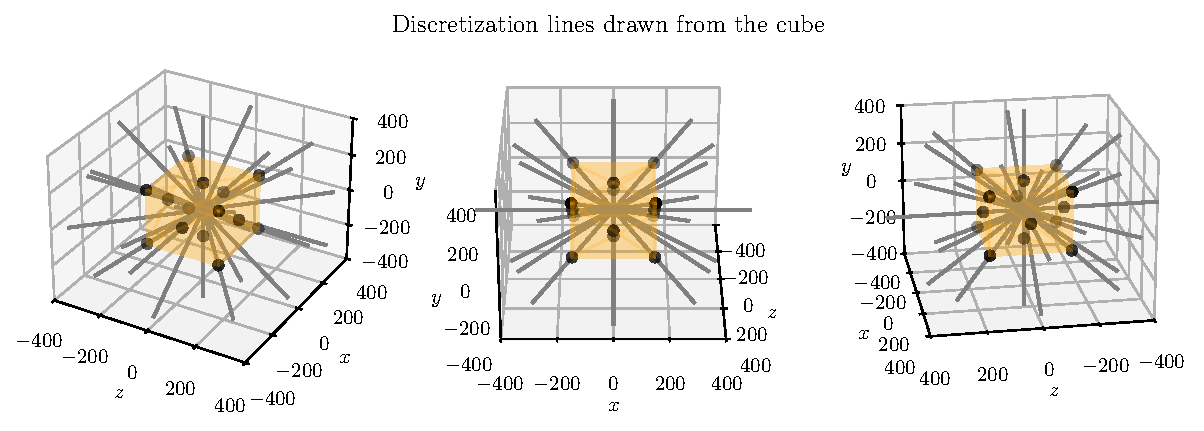
\includegraphics[trim={0 0 0 20}, clip, width=1\linewidth]{img/chapter_4/imgs_discretization/discretization_lines_from_cube.pdf}
    \end{minipage}
    \caption{Three different views of the discretization lines constructed from the cube face lattice. There are 13 lines in total.}
    \label{fig:discretized_directions}
\end{figure}

All these lines intersect at the cube's origin. We shall use them for polytopes to construct $26$ points on a polytope's surface. To ensure that $26$ points are indeed constructable, the lines should intersect at a point located within the polytope. This point is defined to be the barycenter of the polytope's vertices (since it is a convex shape, the barycenter point is located within). However, these constructed lines do not capture how elongated a polytope can be. In this case, most of the formed intersection points are located near the plane generated by the two smaller principal axes of the polytope. These principal axes are constructed from a single value decomposition of the polytope's vertices. Consequently, we shall compute the single value decomposition to retrieve the main polytope's orientation and elongation, and adapt the lines accordingly before starting the intersection process.

The resulting set of $26$ points is termed \emph{discretized polytope} and its construction is shown in figure \ref{fig:polytope_discretization}.

\begin{figure}[!htb]
    \centering
    \captionsetup{justification=centering}
    \begin{minipage}{\linewidth}
        \centering
        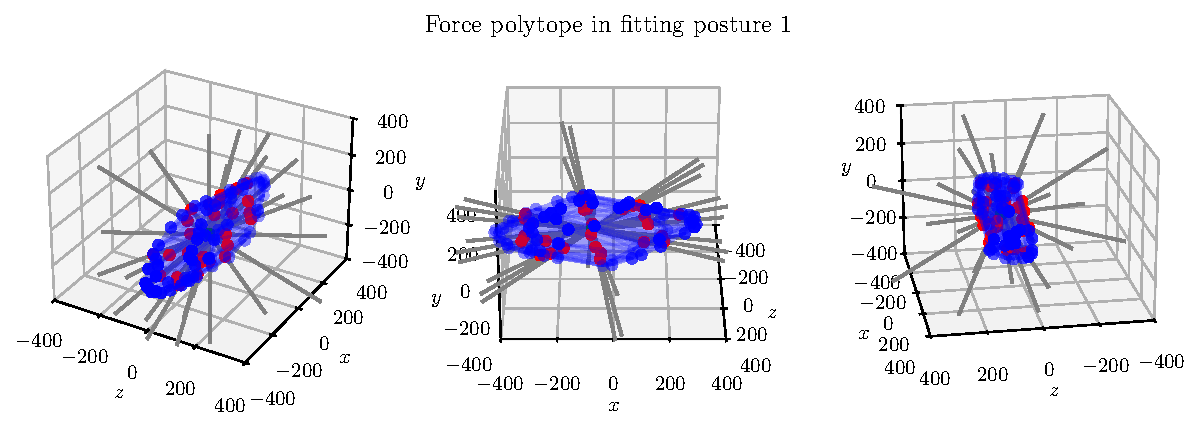
\includegraphics[trim={0 0 0 20}, clip, width=1\linewidth]{img/chapter_4/imgs_discretization/STANFORD_POL_POSTURE_FITTING_01.pdf}
    \end{minipage}
    \caption{Three different views of a force polytope (in blue) and its discretized points (in red), generated by the musculoskeletal model parametrized by Stanford's default muscle values. Units are in Newton. These points are constructed from intersecting lines located at the polytope's barycenter (green point) with the polytope surface.}
    \label{fig:polytope_discretization}
\end{figure}

This has the advantage to prepare for the experimental conditions of gathering maximal isometric force exertions in chapter \ref{chapter:5}, which implies a limited number of force directions to exert.


\paragraph*{Comparing ellipsoidal approximations of force feasible sets.}
While the Hausdorff distance is computationally relevant (to some extent) for polytopal representations of force feasible sets, they are not for ellipsoidal representations: there is no closed-form formula in this case and thus an optimization problem is involved to find the maximum distance between points on two ellipsoids.

If we do not use the Hausdorff distance with ellipsoids, we are left without a distance notion, which is problematic since our optimization problem seeks to find a musculoskeletal model parametrization whose force feasible sets \emph{converge} to the reference force feasible sets. No distance implies no notion of convergence. However, in the eighties, it was shown in (\cite{goffinRelationshipHausdorffDistance1983}) that there are at least two ways to \emph{metrize} the space of ellipsoids \emph{i.e.} to equip it with a distance. The first manner is to use the Hausdorff distance through an optimization. The second manner is to sum the distance between the ellipsoids centers and the distance between their corresponding matrices. 

However, it should be noted that an ellipsoid in 3D is \emph{uniquely defined} through $9$ non-coplanar points on its surface, and even as low as $6$ points if those are located according to the ellipsoid's axes. As such, we consider these 6 points, constructed from the principal axes of an ellipsoid, as shown in figure \ref{fig:ellipsoid_discretization} and the set of these points is termed \emph{discretized ellipsoid}. The Hausdorff distance can thus be applied on two discretized ellipsoids.

\begin{figure}[!htb]
    \centering
    \captionsetup{justification=centering}
    \begin{minipage}{\linewidth}
        \centering
        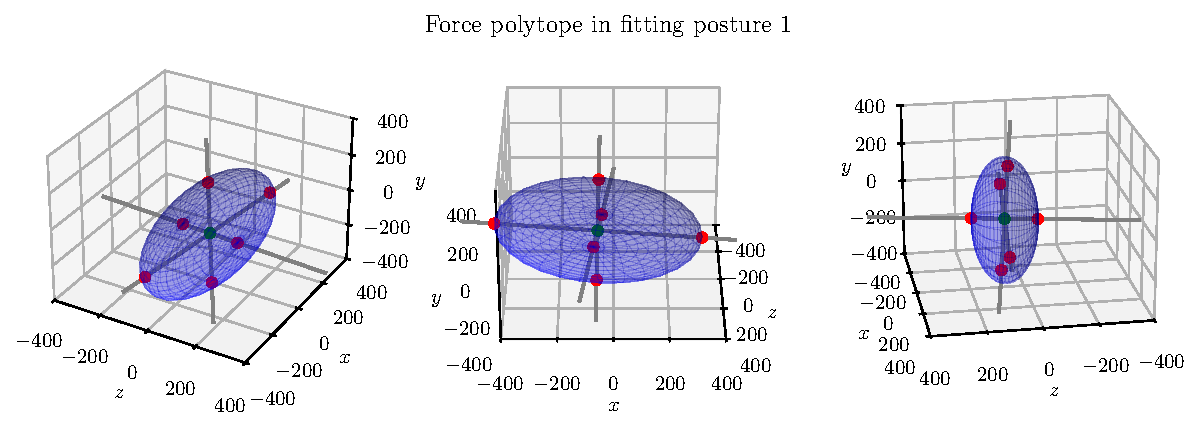
\includegraphics[trim={0 0 0 20}, clip, width=1\linewidth]{img/chapter_4/imgs_discretization/STANFORD_POSTURE_FITTING_01.pdf}
    \end{minipage}
    \caption{Force ellipsoidal approximation (in blue) and its discretized points (in red) of the musculoskeletal model parametrized by Stanford's default muscle values. Units are in Newton. These points are constructed from intersecting the lines of direction this ellipsoid's principal axes and located at the ellipsoid's center (green point).}
    \label{fig:ellipsoid_discretization}
\end{figure}

\paragraph*{Unified comparison function.} We defined a discretized version of polytopes and ellipsoids, so that the Hausdorff distance can be applied on either two polytopes and two ellipsoids.

In the optimization process, this distance is used to compare if two of these shapes are similar. If the distance is $0$ for discretized polytopes, then this indicates that at least $26$ points on both polytope surfaces are located exactly at the same place. Due to the orientation of the lines used to construct them, this means that the barycenters as well as the orientation and elongation of both polytopes are identical. However, nothing could be say about the precise vertices positions, that is why a rather large number of vertices was considered to account for the global shape of polytopes in a reasonnable manner.

For two ellipsoids, since the 6 points present in their discretized version \emph{uniquely} determine them, then a Hausdorff distance of $0$ implies that both ellipsoids are  the same in location, elongation and orientation, which is sufficient to say that both ellipsoids' surfaces coincide.

Finally, we define precisely the comparison function used in the objective function of the previously described optimization problem in \ref{eq:opt_prb}. The distance $d$ is termed \emph{discretized distance} and is defined as follows: for two 3D polytopes or two 3D ellipsoids $\mathcal{F}_1$ and $\mathcal{F}_2$, denote $\mathcal{F}_1^D$ the discretization points set of $\mathcal{F}_1$ and $\mathcal{F}_2^D$ for $\mathcal{F}_2$. Then, 
\begin{align*}
    d(\mathcal{F}_1,\, \mathcal{F}_2) = d_H(\mathcal{F}_1^D,\, \mathcal{F}_2^D)
\end{align*}
where $d_H$ is the Hausdorff distance between two point sets.

\subsection{Handling high-dimensionality, non-differentiability and non-convexity in optimization problems}
\label{subsec:non_differentiability}

Prior to examining optimization solvers, an analysis on the objective function's nature is necessary. Knowledge of its characteristics facilitates the selection of solvers specifically tailored to the its properties. The objective function, while possessing the advantage of explicit computability, exhibits several challenging attributes. These challenges arise primarily from the general force feasible set formulation (independently of a specific tension model $\mathcal{T}$) but also from the set comparison methodology. More precisely, the objective function is non-differentiable, non-convex, and computationally and combinatorially expensive, resulting in a high-dimensional optimization problem.  Nevertheless, efficient solvers have been developed to address such complex optimization problems.

As the force feasible set formulation involves a convex set intersection, the cost function in \ref{eq:opt_prb} is not differentiable. The non-convexity is related to the Hausdorff distance, since it is defined using a $\max$ value, which is not a convex function\footnote{Arguably, in a case where a convex distance or comparison function between two sets is defined, writing the optimization as a convex problem is an added difficult layer due to the geometric formulation of the force feasible sets.}. 

Determining the dimensionality of this optimization problem is usually dependent on the search-space dimension but also on its complexity and the computational expense of evaluating the cost function for a particular solution. Given the heterogeneous parameters encompassing locations (points), lengths (m), and tensions (N), and the relatively high computational cost of objective function evaluation (approximately $250$ ms per force polytope computation using an approximation algorithm as Skuric et al.'s ICH (\cite{skuricOnLineFeasibleWrench2022})), we classify this as a high-dimensional optimization problem. While a simpler musculoskeletal model with fewer parameters could be considered, this would not sufficiently reduce the problem's complexity. Force feasible set comparison remains non-differentiable and non-convex, and computing points on their surfaces remains a combinatorial problem. Furthermore, as demonstrated in chapter \ref{chapter:3}, increasing the number of muscles (and thus parameters) simplifies, rather than complicates, force feasible set representation. Ultimately, the objective of this thesis — applying in silico personalization methods to experimentally measured maximal force exertions — necessitates a complex musculoskeletal model to ensure a generic representation of force feasible sets.

As such, finding a solution requires adapted solving methods. Primarly, they should focus on exploring a large space of solutions but not spend to much computational resources where solutions are not relevant. Two approaches are thus considered and consists of two classes of solving algorithms: the \emph{Genetic Algorithms} (GAs) and \emph{Random Coordinate Shrinking} (RACOS). Both GAs and RACOS belong to the family of derivative-free optimization methods, meaning they can effectively tackle problems where the objective function's derivatives are unavailable or computationally expensive to obtain. Furthermore, both algorithms incorporate elements of randomness in their search strategies, allowing them to escape local optima and explore a wider range of potential solutions.

While they share fundamental characteristics, GAs and RACOS differ in their core mechanisms. GAs maintain a population of solutions and use genetic operators like crossover and mutation to generate new candidate solutions, mimicking natural selection. RACOS, on the other hand, focuses on refining a single solution by iteratively shrinking the search space and leveraging a probabilistic or classification model to guide the search.

This difference in approach makes them complementary in tackling diverse optimization challenges. GAs excel in exploring a vast and complex search space, while RACOS efficiently refines a solution when a promising region has been identified or when evaluations are computationally expensive. The following paragraphs detail in much depth both algorithms.

\paragraph*{Genetic algorithms (GAs).}
Genetic algorithms (GAs) are optimization algorithms inspired by natural selection and first appearance date to 1950, in Turing's paper about machine learning (\cite{turingCOMPUTINGMACHINERYINTELLIGENCE1950}). They effectively address complex problems, particularly those with non-differentiable objective functions or high-dimensional search spaces where gradient-based methods fail. 

GAs iteratively refine a population of candidate solutions (termed \emph{chromosomes}) by evaluating their fitness and applying genetic operators like crossover and mutation. This process guides the population towards optimal solutions, exploiting promising regions of the search space without relying on derivative information. This versatility makes GAs valuable for problems with discrete variables or noisy data where the objective function may be non-differentiable, discontinuous, or computationally expensive to evaluate.

The genetic algorithm begins with a set (\emph{population}) of $n_P$ \emph{individuals} (also termed \emph{chromosomes}), each representing a randomly selected solution $\theta_1, \dots, \theta_{n_P} \in \mathcal{X}$ from the search space $\mathcal{X}$ of optimization problem \ref{eq:opt_prb}. Each chromosome, composed of \emph{genes} (representing the coordinate values of a solution $\theta$), is evaluated using the cost function. This involves parameterizing Stanford's model and computing force feasible sets for the predefined postures in $\mathcal{Q}$. We recall that the cost function quantifies the dissimilarity between the computed and target force feasible sets across all postures in $\mathcal{Q}$.

The algorithm proceeds through $n_G$ \emph{generations}, iteratively creating new populations. In each generation, a \emph{selection process}, such as selecting the 5 best-performing chromosomes, identifies parent individuals. With probability $c_r$, two parents undergo crossover, combining their genes to produce offspring. An \emph{arithmetic} crossover strategy, employing a weighted average of parent genes, can be of interest for real-valued chromosomes. Subsequently, each offspring undergoes mutation with probability $m_r$, introducing small perturbations to their genes, potentially adapted to the physical meaning of the parameters (\emph{e.g.},  perturbing origin/insertion points uniformly, and optimal fiber length with a Gaussian distribution). \emph{Adaptive mutation} may be employed, reducing perturbation magnitudes as the algorithm progresses.

The fitness of the offspring is then evaluated, and a new population is formed, optionally including a subset of the parents. This process iterates until a termination criterion (\emph{e.g.}, achieving a cost function value below $10^{-3}$) is met or all generations are completed. The best solution from the final population is then returned (see Algorithm \ref{alg:genetic_algorithm} for a pseudo-code summary).

\begin{figure}[!ht]
    \centering
    \begin{minipage}{1.0\linewidth}
        \begin{algorithm}[H]
            \SetAlgoLined
            \KwData{Population size $n_P$, Crossover rate $c_r$, Mutation rate $m_r$, Maximum generations $n_G$}
            \KwResult{Best solution found}
            
            \BlankLine
            
            \textbf{Initialize} population randomly with $P$ individuals\;
            \For{each individual}{
                \textbf{Evaluate} fitness of the individual\;
            }
            
            \For{generation = 1 to $n_G$}{
                \textbf{Select} parents from the population based on fitness\;
                \While{new population size $< n_P$}{
                    \textbf{Crossover}: with probability $c_r$, crossover two parents to produce two offspring\;
                    \textbf{Mutate}: with probability $m_r$, mutate offspring\;
                    \textbf{Evaluate} fitness of offspring\;
                    \textbf{Add} offspring to the new population\;
                }
                \textbf{Replace} old population with the new population\;
                
                \If{termination condition is met}{
                    \textbf{break}\;
                }
            }
            \Return{Best solution from the population}
            \caption{Genetic Algorithm}
            \label{alg:genetic_algorithm}
        \end{algorithm}
    \end{minipage}
\end{figure}

Although genetic algorithms offer flexibility in strategy selection, effective implementation relies on an understanding of the search space structure (specifically its \emph{topology}). Given our limited knowledge of the specific influence of individual muscle parameters on force feasible set generation (we can only characterize how the complete parameter set collectively determines the force feasible sets), we aim to explore the search space topology concurrently with solution sampling. To address the limitations of genetic algorithms in navigating complex search spaces with poorly understood parameter influences, we employ the \emph{Random Coordinate Shrinking} algorithm (\cite{yuDerivativeFreeOptimizationClassification2016}). This algorithm constructs a probabilistic model during search space exploration to assess the quality of a solution based on its location in the search space $\mathcal{Q}$. This model-guided approach facilitates efficient exploration and exploitation of the search space, particularly when the relationship between individual parameters and the objective function is unclear.

\paragraph*{Random Coordinate Shrinking (RACOS).}
In contrast to GAs' approach, RACOS methods utilize an iterative framework that involves learning a model to identify promising search areas and subsequently sampling new solutions from this model. The \emph{Random Coordinate Shrinking} algorithm (RACOS) (\cite{yuDerivativeFreeOptimizationClassification2016}) adheres to this framework, employing a classification model to distinguish between high-performing and low-performing solutions.

RACOS leverages this probabilistic model by iteratively refining a solution by shrinking the search space around it. It operates by randomly selecting a coordinate within the current search space and optimizing the solution along that coordinate. This process is repeated until the search space converges to a small region, indicating the location of a near-optimal solution. The algorithm is presented in details in algorithm \ref{alg:racos}.

\begin{figure}[!ht]
    \centering
    \begin{minipage}{1.0\linewidth}
        \begin{algorithm}[H]
            \SetAlgoLined
            \KwData{Search space $\mathcal{X}$ of dimension $d$, number of iterations $n$, sample size $N$, positive sample size $k$, budget $B$}
            \KwResult{Best solution found}
            \BlankLine
            
            \textbf{Initialize} sample set $P$ with $N$ random samples from $\mathcal{X}$\;
            \textbf{Evaluate} the fitness of each sample in $P$\;
            \textbf{Sort} $P$ based on fitness\;
            \textbf{Select} top $k$ samples as the positive set $P_+$\;
            Let $\theta_{best}$ be the best solution from $P_+$\;
            \BlankLine
            
            \For{$t = 1$ to $n$}{
                \For{$i = 1$ to $N$}{
                    \textbf{Randomly generate} a new sample $\theta_{new}$ by randomized sampling\;
                    \For{each dimension $j = 1$ to $d$}{
                        \textbf{Randomly decide} whether to sample within the region defined by the positive set $P_+$\;
                        \If{within region}{
                            Generate value for $\theta_{new}[j]$ based on the distribution defined by $P_+$\;
                        }
                        \Else{
                            Generate value for $\theta_{new}[j]$ uniformly from the search space\;
                        }
                    }
                    \textbf{Evaluate} the fitness of $\theta_{new}$\;
                    \If{$\theta_{new}$ is better than the worst in $P_+$}{
                        Replace the worst sample in $P_+$ with $\theta_{new}$\;
                        \If{$\theta_{new}$ is better than $\theta_{best}$}{
                            Update $\theta_{best}$ with $\theta_{new}$\;
                        }
                    }
                }
            }
            \Return{$\theta_{best}$ as the best solution found}
            \caption{RACOS algorithm (Randomized Coordinate Sampling)}
            \label{alg:racos}
        \end{algorithm}
\end{minipage}
\end{figure}

The probabilistic model in SRACOS serves two primary purposes. First, it guides the search by prioritizing coordinates with high uncertainty or potential for improvement. Second, it facilitates informed decision-making by providing estimates of the objective function value at unsampled locations. This capability allows RACOS to efficiently explore the search space and exploit promising regions.

Unlike GAs, which rely on population-based genetic operators, RACOS's probabilistic model enables a more focused and informed search strategy. This approach is particularly advantageous in high-dimensional or complex optimization landscapes, where efficiently exploring the search space is crucial.


\paragraph*{Implementation of solvers and force feasible sets computation in Python.} 
All scripts, written in Python 3.10, were executed on the PlaFRIM experimental testbed\footnote{PlaFRIM (Inria, CNRS, LABRI, IMB, Université de Bordeaux, Bordeaux INP and Conseil Régional d'Aquitaine). See \url{https://www.plafrim.fr}.}. This platform enabled parallelized computation of polytopes across multiple postures, as well as repetition of a test over different machines. The utilized machines feature 2x32-core AMD Zen2 EPYC 7452 CPUs (at 2.35 GHz).

Both solvers, the genetic algorithm and SRACOS, are implemented in Python 3 using the PyGAD\footnote{\url{https://pygad.readthedocs.io/en/latest/}} (\cite{gadPyGADIntuitiveGenetic2021}) and ZOOpt\footnote{\url{https://zoopt.readthedocs.io/en/latest/}} (\cite{liuZOOptToolboxDerivativeFree2022}) packages, respectively.
 
Force feasible sets, modeled as polytopes, are computed using the Iterative Convex Hull method presented in (\cite{skuricOnLineFeasibleWrench2022}) implemented in the \emph{pycapacity}\footnote{\url{https://auctus-team.github.io/pycapacity/}} package (\cite{skuricPycapacityRealtimeTaskspace2023}). A tolerance of 1 or 5 Newtons is employed depending on the specific case.

Ellipsoidal approximations of the force polytopes are generated using our custom \emph{hyperobjects}\footnote{\url{https://gitlab.inria.fr/auctus-team/people/gautierlaisne/public/hyperobjects}} package, which computes the resulting ellipsoid from the projection or intersection of any $m$-dimensional ellipsoid with a lower $n$-dimensional affine subspace.

\subsection{Assessing the accuracy of fitted personalized musculoskeletal models}
\label{subsec:validation_optimization_pb}

After the determination of a solution, it is essential to evaluate its capacity to reproduce expected force feasible sets in postures not included in the objective function. While considering all possible postures would be ideal, experimental limitations restrict the acquisition of maximal isometric force exertions to one posture at a time. Consequently, both the reference posture set $\mathcal{Q}$ and the validation posture set $\mathcal{Q}_{val}$ contain a limited number of postures.

Determining the precise number of postures required for accurate muscle parameter identification from force feasible sets remains an open question. Therefore, guided by experimental constraints, we restrict our analysis to approximately 4 postures or fewer. Chapter \ref{chapter:5} elaborates on the experimental challenges that preclude the consideration of a larger number of postures.

To assess the impact of this limitation, sections \ref{sec:personalization_silico_polytopes} and \ref{sec:personalization_silico_ellipsoid} investigate the feasibility of solving the optimization problem with 3, 4, and 6 reference postures. In silico analysis will demonstrate that increasing the number of postures directly enhances the quality of the obtained solution. However, in the case of ellipsoidal force feasible set approximations, it will be shown that only 3 postures are necessary to achieve a satisfactory solution.

\paragraph*{Quantitative assessment.} The accuracy of a solution depends on two parts: on one hand the \emph{fitting} process is evaluated so that for each considered fitting posture $\mathbf{q}\in\mathcal{Q}$, the produced force feasible sets produced by the found solution are compared respectively with the force feasible set to fit. Various metrics are used for this comparison, involving all those described in the subsection about force feasible set comparison in \ref{subsec:comparing_ffs}.

Similarly, this method is applied for other postures defined in $\mathcal{Q}_{val}$. We are in a simulation context, so it can be assumed that we also know the force feasible sets of Stanford's model for postures in $\mathcal{Q}_{val}$.

Comparing the produced force feasible sets to the expected ones in the fitting postures as well as the validation postures allows us to evaluate if a solution is overfitting or underfitting, and allows us to gauge how many postures are required until a solution recreate the force feasible sets in any posture. 

\paragraph*{Qualitative assessment.} While it is, comparing 3D convex shape is also straight-forward qualitatively and is an important part of measuring the correspondance between two sets. So, while sometimes quantitative values can describe a large difference between two sets, the sets can still be very close (in shape, elongation, orientation, and size) as it was shown in figure \ref{fig:hausdorff_sensitivity}, where noise has a negative impact on the interpretation of quantitative results. 

\section{Muscle parameters sensitivity via force polytopes}
\label{sec:personalization_silico_polytopes}

Having formally defined the optimization problem, we focus on its implementation. The problem definition in section \ref{sec:musculoskeletal_model_muscle_pers_sec} raises several key questions:

\begin{itemize}[noitemsep]
    \item {How does the number of postures affect the quality of the obtained solution?}
    \item {What is the maximum size of the search space that guarantees convergence to a solution?}
    \item {How does the force feasible set representation influence convergence towards an optimal solution?}
\end{itemize}

Furthermore, we aim to evaluate multiple solving methods and identify the most effective approach with respect to the aforementioned questions. Besides, we seek to determine whether polytopic and ellipsoidal representations are interchangeable within the optimization process.

To address these questions, we define a set of \emph{hyperparameters} that configure the optimization problem into sub-problems. Each sub-problem addresses specific question, namely: the influence of the number of postures on the results, the maximum feasible search space size, the relative performance of different solvers and the impact of the force feasible set representation on solution discovery.

\subsection{Hyperparameters optimization}

A \emph{hyperparameter} is a parameter that influences the optimization process itself, but is not directly optimized by the process. It is established prior to optimization and significantly influences the process's efficiency and effectiveness, affecting aspects such as search space exploration, convergence speed, and the quality of the final solution.

Based on empirical intuition and prior analyses (\cite{laisneGeneticAlgorithmsForce2023}; \cite{laisneDerivativeFreeOptimizationApproaches2023}), we consider five hyperparameters:

\begin{enumerate}
    \item \textbf{Force feasible set representation:} this hyperparameter dictates the representation of the force feasible sets, utilizing either force polytopes or their ellipsoidal approximations;
    \item \textbf{Optimization solver:} two distinct optimization solvers are employed (a genetic algorithm and RACOS);
    \item \textbf{Number of fitting postures:} the force feasible sets are computed for each posture using either 3 postures (posture set $\mathcal{Q}_3^{\text{fit}}$) or 6 postures (posture set $\mathcal{Q}_6^{\text{fit}}$). These posture sets are termed \emph{fitting postures} as they are used to \emph{fit} the produced force feasible set of a solution;
    \item \textbf{Muscle parameter type perturbation:} this hyperparameter defines the type of muscle parameter concerned by the optimization, \emph{i.e.} the solution consists of only values of a certain type. Each muscle parameter belongs to a specific type: maximal isometric force ($f_{iso}$), optimal fiber length ($l_o$), tendon slack length ($l_s$), pennation angle ($\alpha$), and points defining the muscle path. To analyze the influence of each parameter type on the force feasible sets, we perturb all muscles' parameters of a single type. For instance, all muscles' maximal isometric forces are perturbed, or all optimal fiber lengths, and so on. Additionally, we consider two combinations of parameters: perturbations of 1) $f_{iso}$, $l_o$, and $l_s$ parameters and 2) $f_{iso}$, $l_o$, $l_s$, and muscle geometry parameters;
    \item \textbf{Search space size:} for each selected parameter type, three search spaces of varying sizes are considered and termed \emph{large}, \emph{medium}, and \emph{small}. These search spaces are centered around each muscle parameter and their specific values are detailed in the preceding section.
\end{enumerate}

All possible hyperparameter combinations result in $168$ distinct cases. Due to the stochastic nature of the solvers' solution selection, each optimization case is repeated $5$ times to ensure solution discovery and assess process repeatability. This leads to a total of $840$ optimization runs.

A detailed explanation of each hyperparameter follows.

\paragraph*{Force feasible sets representation.} This section presents the first feasible set representation: the \emph{force polytope}, which corresponds to force feasible sets modeled using a $\mathcal{T}_{\infty}$ tension set model. Next section will subsequently examine the ellipsoidal approximation of these force polytopes. Separate sections are dedicated to each representation due to differences in the interpretation of the distance function used for comparing force feasible sets. These differences stem from the varying number of points sampled on the force feasible set surface during the discretization process.

\paragraph*{Optimization solver.} We shall consider either a genetic algorithm or a more recent approach, RACOS, which tries to learn how the search space is structured.

The genetic algorithm is initialized with a population of 1000 solutions. In each generation, 5 parents are selected for crossover using a single-point strategy.  This strategy involves dividing the chromosomes of two parent solutions into two parts (with a 0.5 probability of a cut at any specific gene) and creating a new solution by combining the first part of the first parent with the second part of the second parent. This mechanism induces greater variability within the population.  An \emph{adaptive} mutation process is employed, with a probability of 0.8 for low-quality solutions and 0.2 for high-quality solutions. The subsequent generation comprises 10 solutions: the 2 best parents, 3 crossovers generated from the 5 selected parents, and 5 mutations derived from these crossovers.

When using RACOS, the solver process is initiated by running RACOS 5 times, each with a random initial population of 10 solutions, for a duration of 5 or 10 minutes, depending on the parameters being considered (see the following paragraph for details). These initial runs generate solutions that are widely distributed within the search space, which is crucial for addressing the high dimensionality of the problem, similarly to the goal of the single-point crossover in the genetic algorithm. Thereafter, a sixth RACOS solver is executed, with its initial population consisting of the 5 solutions obtained in the previous runs. All RACOS implementations utilize the default parameters defined in the Python package \emph{Zoopt} (\cite{yuDerivativeFreeOptimizationClassification2016}), as this configuration has been empirically determined to be most effective.

Both solvers terminate based on a time-based criterion that depends on the muscle parameters under consideration. For $f_{iso}$, $l_o$, $l_s$ or $\alpha$, the total solving process is halted after 30 minutes. For the muscle geometry case and the combination of $f_{iso}$, $l_o$ and $l_s$, optimization ceases after 2 hours. In the most challenging scenario (dimensionality-wise), where $f_{iso}$, $l_o$, $l_s$ and all muscle parameters are considered together, the termination time is extended to 4 hours.

\paragraph*{Number of fitting postures.}
In order to gauge how the number of postures influences the quality of a found solution, two sets of postures are considered.

The first includes $3$ postures $\mathbf{q}_1^{\text{fit}}$, $\mathbf{q}_2^{\text{fit}}$ and $\mathbf{q}_3^{\text{fit}}$, which have been arbitrarily chosen but produce qualitatively different force feasible sets (in orientation mainly) and ensures that the upper limb postures are diverse in the workspace. The set of these $3$ postures is denoted $\mathcal{Q}_3^{\text{fit}}= \left\{\mathbf{q}_1^{\text{fit}}, \mathbf{q}_2^{\text{fit}}, \mathbf{q}_3^{\text{fit}}\right\}$. Choosing only $3$ postures accounts for the experimental difficulties of gathering maximal force exertions in a given postures, as it will be more detailed in chapter \ref{chapter:5}. 

Nevertheless, only 3 postures may not sufficiently capture muscle relations to obtain a good solution. It is thus relevant to asses if, outside of the future experimental considerations, a higher number of postures could have a significant advantage over the prediction quality of a solution. However, the higher the number of postures, the more time-expensive the solving is. Consequently, we limit ourselves to a second set of postures, denoted $\mathcal{Q}_6^{\text{fit}}$, which corresponds to $6$ postures including the set postures in $\mathcal{Q}_3^{\text{fit}}$.

\paragraph*{\underline{3 fitting postures $\mathcal{Q}_3^{\text{fit}}$}:}
The following table \ref{tab:postures_fit_3_value} and figures \ref{fig:pose_1}, \ref{fig:pose_2} and \ref{fig:pose_3} describe the posture parametrizations of $\mathbf{q}_1^{\text{fit}}$, $\mathbf{q}_2^{\text{fit}}$ and $\mathbf{q}_3^{\text{fit}}$ respectively.

\begin{table}[!ht]
    \centering
    \begin{tabular}{|c||c|c|c|c|c|c|c|}
    \hline
    Posture & \makecell{Elevation \\ angle} & \makecell{Shoulder \\ elevation} & \makecell{Shoulder \\ rotation} & \makecell{Elbow \\flexion} & \makecell{Pronation \\ supination} & \makecell{Wrist \\ deviation} & \makecell{Wrist \\ flexion} \\
    \hline
    $\mathbf{q}_1^{\text{fit}}$ & $62$° & $35$° & $19$° & $80$° & $-1$° & $-0.126$ & $-0.632$ \\
    $\mathbf{q}_2^{\text{fit}}$ & $16$° & $92$° & $22$° & $72$° & $2$° & $0.014$ & $-0.408$ \\
    $\mathbf{q}_3^{\text{fit}}$ & $86$° & $74$° & $95$° & $58$° & $-25$° & $0.007$ & $-0.127$ \\
    \hline
    \end{tabular}
    \caption{Fitting postures parametrization in $\mathcal{Q}_3^{\text{fit}}$. All values in degrees are expressed in radians in OpenSim. The wrist deviation and flexion values are defined to be in a small subset of $[-1,1]$. They serve as an underlying parametrization of the wrist deviation and flexion angles in the considered musculoskeletal model.}
    \label{tab:postures_fit_3_value}
\end{table}

Figures \ref{fig:pose_1}, \ref{fig:pose_2} and \ref{fig:pose_3} show the 3 fitting postures in the above-mentionned order, in three different views in order to grasp the 3D representation.
\begin{figure}[!htb]
    \centering
    \captionsetup{justification=centering}
    \begin{minipage}{0.3\linewidth}
        \centering
        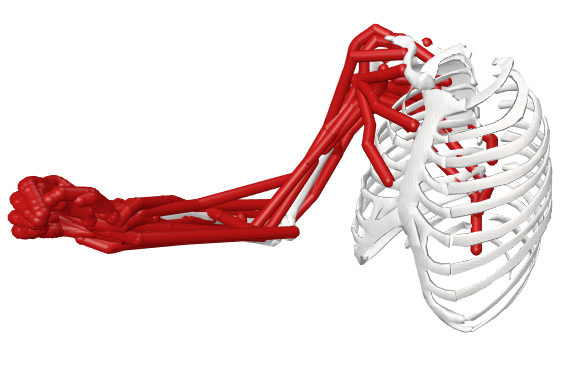
\includegraphics[trim={0 0 0 0}, clip, width=0.95\linewidth]{img/chapter_4/pose_1_view.png}
    \end{minipage}
    \hfill
    \begin{minipage}{0.3\linewidth}
        \captionsetup{justification=centering}
        \centering
        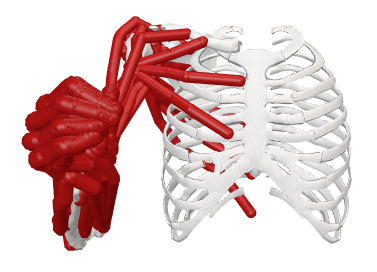
\includegraphics[trim={0 0 0 0}, clip, width=0.75\linewidth]{img/chapter_4/pose_1_front.png}
    \end{minipage}
    \hfill
    \begin{minipage}{0.3\linewidth}
        \captionsetup{justification=centering}
        \centering
        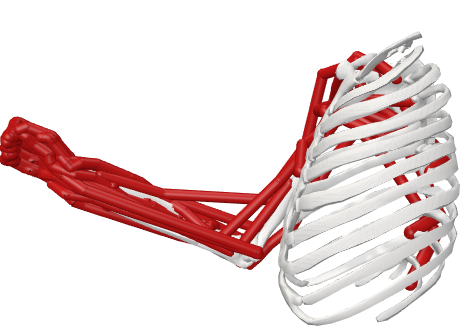
\includegraphics[trim={0 0 0 0}, clip, width=0.8\linewidth]{img/chapter_4/pose_1_side.png}
    \end{minipage}
    \caption{Fitting posture $\mathbf{q}_1^{\text{fit}}$.}
    \label{fig:pose_1}
\end{figure}

\begin{figure}[!htb]
    \centering
    \captionsetup{justification=centering}
    \begin{minipage}{0.3\linewidth}
        \centering
        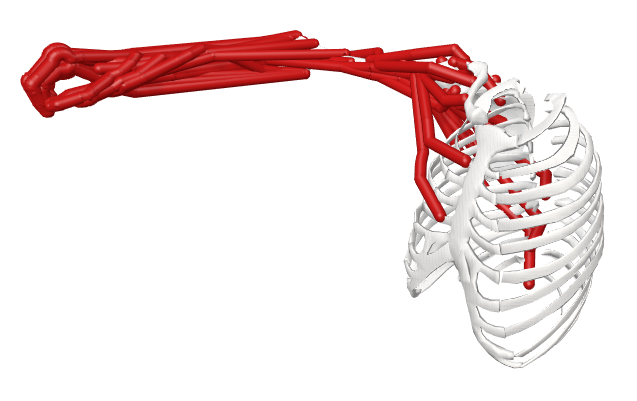
\includegraphics[trim={0 0 0 0}, clip, width=1\linewidth]{img/chapter_4/pose_4_view.png}
    \end{minipage}
    \hfill
    \begin{minipage}{0.3\linewidth}
        \captionsetup{justification=centering}
        \centering
        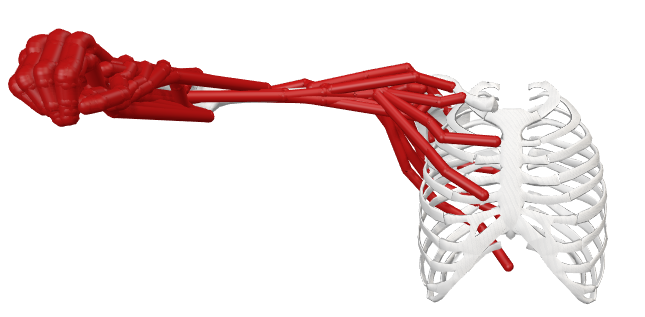
\includegraphics[trim={10 0 0 0}, clip, width=1\linewidth]{img/chapter_4/pose_4_front.png}
    \end{minipage}
    \hfill
    \begin{minipage}{0.3\linewidth}
        \captionsetup{justification=centering}
        \centering
        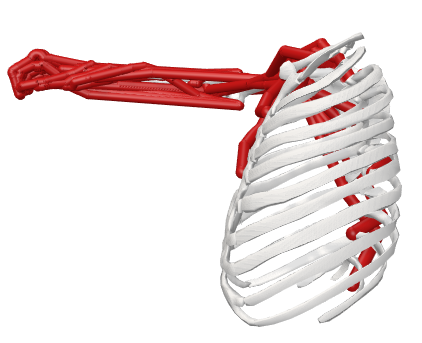
\includegraphics[trim={0 0 0 0}, clip, width=0.72\linewidth]{img/chapter_4/pose_4_side.png}
    \end{minipage}
    \caption{Fitting posture $\mathbf{q}_2^{\text{fit}}$.}
    \label{fig:pose_2}
\end{figure}

\begin{figure}[!htb]
    \centering
    \captionsetup{justification=centering}
    \begin{minipage}{0.3\linewidth}
        \centering
        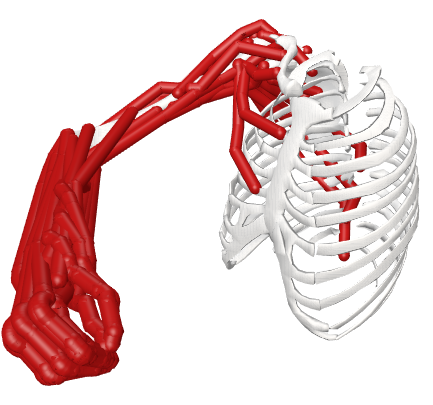
\includegraphics[trim={0 0 0 0}, clip, width=0.7\linewidth]{img/chapter_4/pose_6_view.png}
    \end{minipage}
    \hfill
    \begin{minipage}{0.3\linewidth}
        \captionsetup{justification=centering}
        \centering
        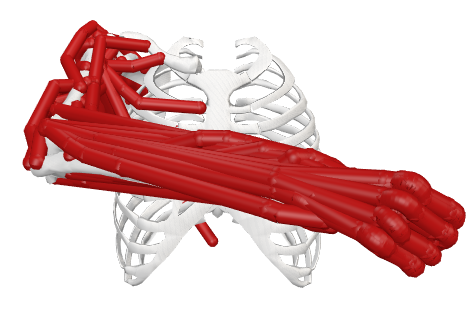
\includegraphics[trim={0 0 0 0}, clip, width=0.8\linewidth]{img/chapter_4/pose_6_front.png}
    \end{minipage}
    \hfill
    \begin{minipage}{0.3\linewidth}
        \captionsetup{justification=centering}
        \centering
        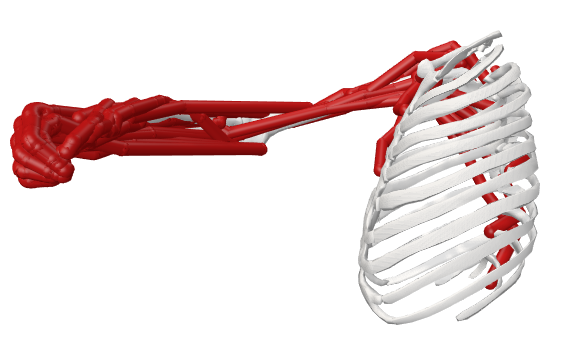
\includegraphics[trim={10 0 0 0}, clip, width=0.9\linewidth]{img/chapter_4/pose_6_side.png}
    \end{minipage}
    \caption{Fitting posture $\mathbf{q}_3^{\text{fit}}$.}
    \label{fig:pose_3}
\end{figure}

For each of these postures, their respective force polytope is computed using Skuric et al. Iterative Convex Hull algorithm with a tolerance of $5$ Newton (\cite{skuricOnLineFeasibleWrench2022}). We shall show their shape in figures \ref{fig:polytope_pose_1}, \ref{fig:polytope_pose_2} and \ref{fig:polytope_pose_3}, using multiple views to emphasize its dimensionality. The frame used corresponds to the global frame in OpenSim, where the $y$-axis is normal to the transversal plane, the $x$-axis normal to the coronal plane and the $z$-axis normal to the sagittal plane.

\clearpage
\begin{figure}[!htb]
    \centering
    \captionsetup{justification=centering}
    \begin{minipage}{\linewidth}
        \centering
        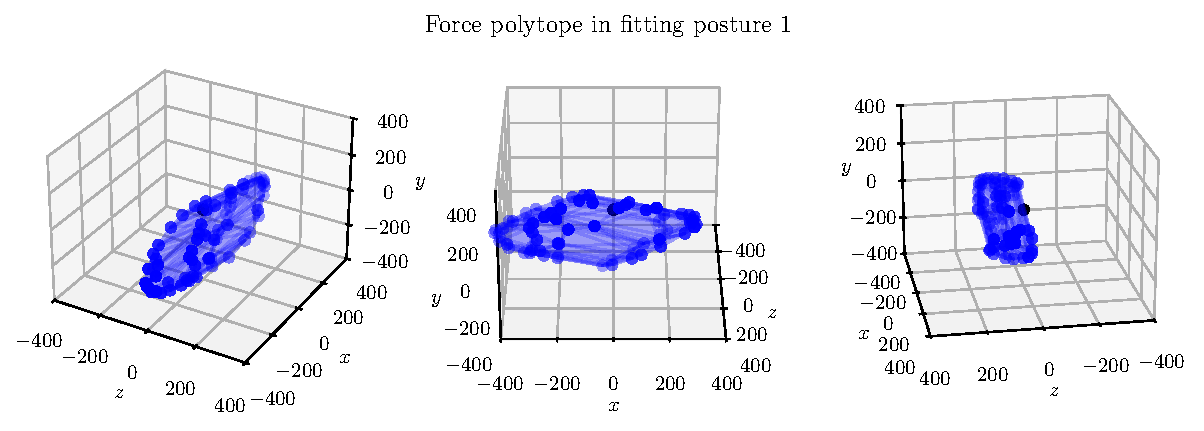
\includegraphics[trim={0 0 0 0}, clip, width=1\linewidth]{img/chapter_4/reconstruction_stanford_imgs/STANFORD_POSTURE_FITTING_01.pdf}
    \end{minipage}
    \caption{Force polytope of the musculoskeletal model parametrized by Stanford's default muscle values in fitting posture $\mathbf{q}_1^{\text{fit}}$. Units are in Newton.}
    \label{fig:polytope_pose_1}
\end{figure}

\begin{figure}[!htb]
    \centering
    \captionsetup{justification=centering}
    \begin{minipage}{\linewidth}
        \centering
        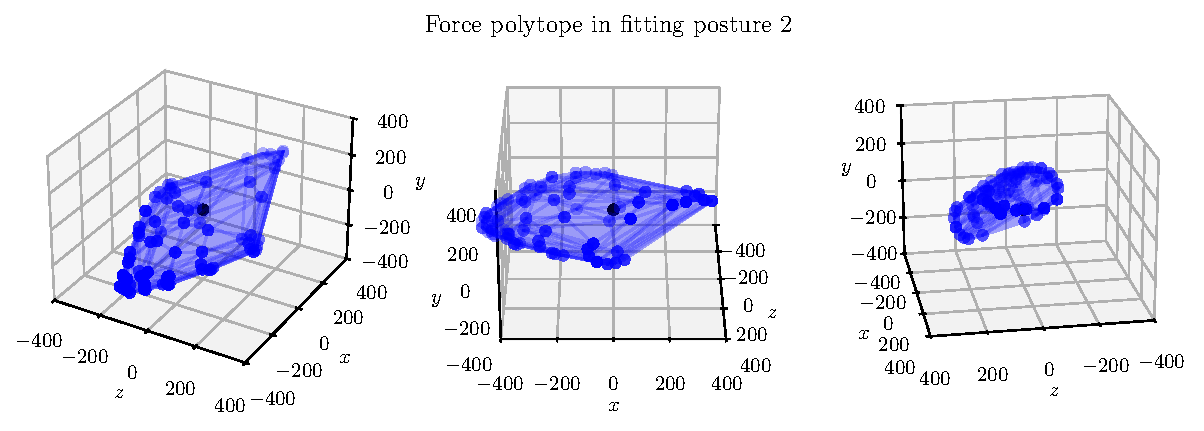
\includegraphics[trim={0 0 0 0}, clip, width=1\linewidth]{img/chapter_4/reconstruction_stanford_imgs/STANFORD_POSTURE_FITTING_02.pdf}
    \end{minipage}
    \caption{Force polytope of the musculoskeletal model parametrized by Stanford's default muscle values in fitting posture $\mathbf{q}_2^{\text{fit}}$. Units are in Newton.}
    \label{fig:polytope_pose_2}
\end{figure}

\begin{figure}[!htb]
    \centering
    \captionsetup{justification=centering}
    \begin{minipage}{\linewidth}
        \centering
        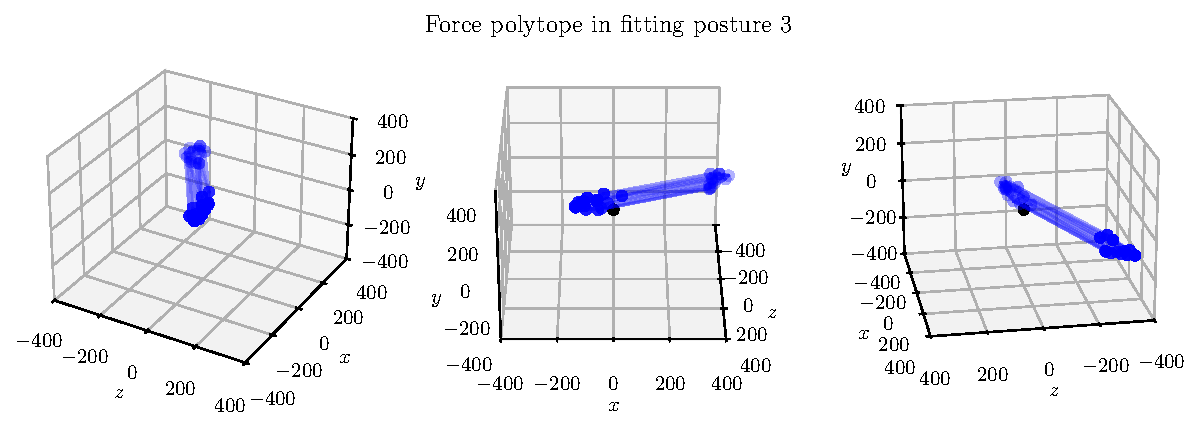
\includegraphics[trim={0 0 0 0}, clip, width=1\linewidth]{img/chapter_4/reconstruction_stanford_imgs/STANFORD_POSTURE_FITTING_03.pdf}
    \end{minipage}
    \caption{Force polytope of the musculoskeletal model parametrized by Stanford's default muscle values in fitting posture $\mathbf{q}_3^{\text{fit}}$. Units are in Newton.}
    \label{fig:polytope_pose_3}
\end{figure}

\clearpage
\paragraph*{\underline{6 fitting postures $\mathcal{Q}_6^{\text{fit}}$:}}
In a similar manner as the previous description, table \ref{tab:postures_fit_6_value} and figures \ref{fig:pose_4}, \ref{fig:pose_5} and \ref{fig:pose_6} show how the 3 additionnal postures in $\mathcal{Q}_6^{\text{fit}} = \mathcal{Q}_3^{\text{fit}} \cup \left\{\mathbf{q}_4^{\text{fit}}, \mathbf{q}_5^{\text{fit}}, \mathbf{q}_6^{\text{fit}}\right\}$ are represented. Figures \ref{fig:pose_4}, \ref{fig:pose_5} and \ref{fig:pose_6} show the 3 additionnal fitting postures and figures \ref{fig:polytope_pose_4}, \ref{fig:polytope_pose_5} and \ref{fig:polytope_pose_6} their associated computed force polytopes.

\begin{table}[!htb]
    \centering
    \begin{tabular}{|c||c|c|c|c|c|c|c|}
    \hline
    Posture & \makecell{Elevation \\ angle} & \makecell{Shoulder \\ elevation} & \makecell{Shoulder \\ rotation} & \makecell{Elbow \\flexion} & \makecell{Pronation \\ supination} & \makecell{Wrist \\ deviation} & \makecell{Wrist \\ flexion} \\
    \hline
    $\mathbf{q}_1^{\text{fit}}$ & $62$° & $35$° & $19$° & $80$° & $-1$° & $-0.126$ & $-0.632$ \\
    $\mathbf{q}_2^{\text{fit}}$ & $16$° & $92$° & $22$° & $72$° & $2$° & $0.014$ & $-0.408$ \\
    $\mathbf{q}_3^{\text{fit}}$ & $86$° & $74$° & $95$° & $58$° & $-25$° & $0.007$ & $-0.127$ \\
    
    $\mathbf{q}_4^{\text{fit}}$ & $40$° & $38$° & $39$° & $61$° & $-58$° & $0.000$ & $0.000$ \\
    $\mathbf{q}_5^{\text{fit}}$ & $75$° & $91$° & $50$° & $101$° & $-50$° & $0.000$ & $0.000$ \\
    $\mathbf{q}_6^{\text{fit}}$ & $75$° & $76$° & $50$° & $50$° & $-3$° & $0.028$ & $0.000$ \\
    \hline
    \end{tabular}
    \caption{Fitting postures parametrization for the second posture set $\mathcal{Q}_6^{\text{fit}}$. The three first postures are identical to those in $\mathcal{Q}_3^{\text{fit}}$.}
    \label{tab:postures_fit_6_value}
\end{table}

\begin{figure}[!htb]
    \centering
    \captionsetup{justification=centering}
    \begin{minipage}{0.3\linewidth}
        \centering
        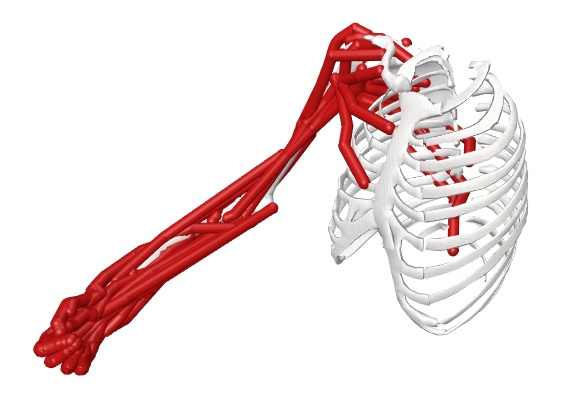
\includegraphics[trim={0 0 0 0}, clip, width=0.9\linewidth]{img/chapter_4/pose_9_view.png}
    \end{minipage}
    \hfill
    \begin{minipage}{0.3\linewidth}
        \captionsetup{justification=centering}
        \centering
        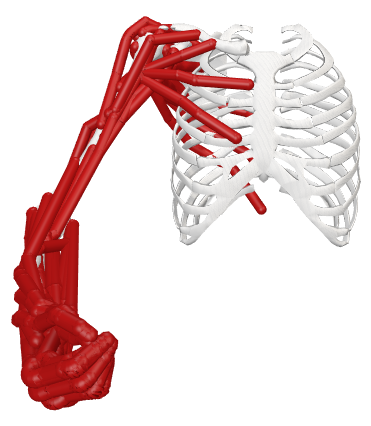
\includegraphics[trim={0 0 0 0}, clip, width=0.7\linewidth]{img/chapter_4/pose_9_front.png}
    \end{minipage}
    \hfill
    \begin{minipage}{0.3\linewidth}
        \captionsetup{justification=centering}
        \centering
        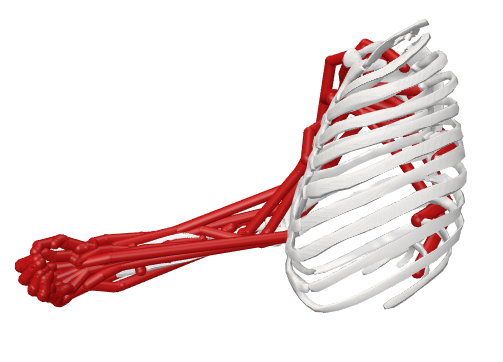
\includegraphics[trim={0 0 0 0}, clip, width=0.9\linewidth]{img/chapter_4/pose_9_side.png}
    \end{minipage}
    \caption{Fitting posture $\mathbf{q}_4^{\text{fit}}$.}
    \label{fig:pose_4}
\end{figure}

\begin{figure}[!htb]
    \centering
    \captionsetup{justification=centering}
    \begin{minipage}{0.3\linewidth}
        \centering
        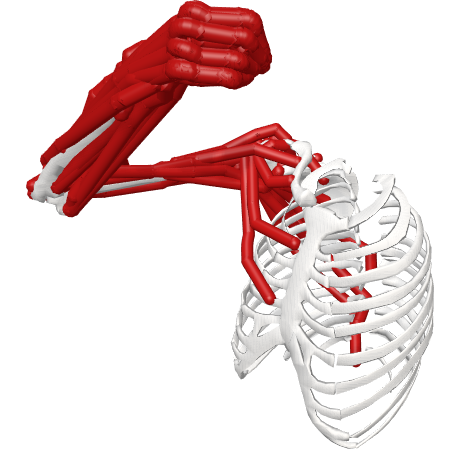
\includegraphics[trim={0 0 0 0}, clip, width=0.8\linewidth]{img/chapter_4/pose_3_view.png}
    \end{minipage}
    \hfill
    \begin{minipage}{0.3\linewidth}
        \captionsetup{justification=centering}
        \centering
        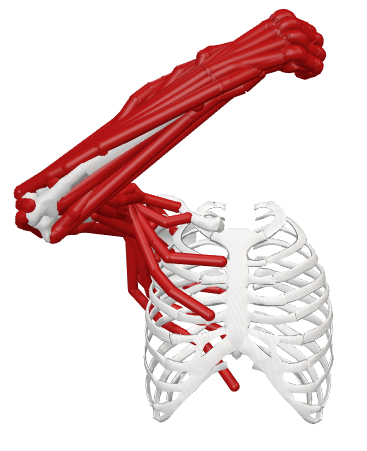
\includegraphics[trim={0 0 0 0}, clip, width=0.7\linewidth]{img/chapter_4/pose_3_front.png}
    \end{minipage}
    \hfill
    \begin{minipage}{0.3\linewidth}
        \captionsetup{justification=centering}
        \centering
        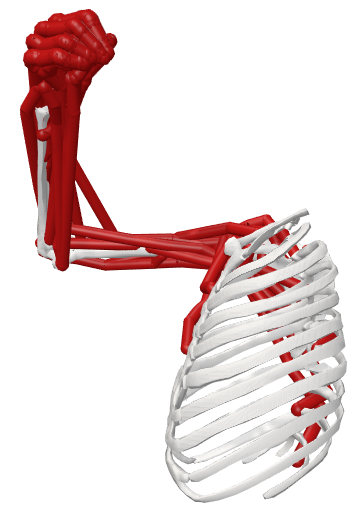
\includegraphics[trim={0 0 0 0}, clip, width=0.6\linewidth]{img/chapter_4/pose_3_side.png}
    \end{minipage}
    \caption{Fitting posture $\mathbf{q}_5^{\text{fit}}$.}
    \label{fig:pose_5}
\end{figure}

\begin{figure}[!htb]
    \centering
    \captionsetup{justification=centering}
    \begin{minipage}{0.3\linewidth}
        \centering
        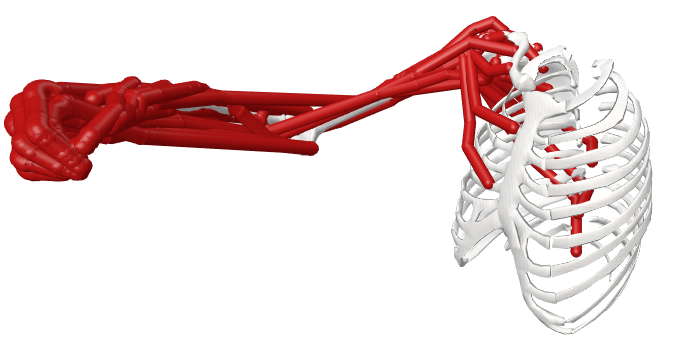
\includegraphics[trim={10 10 10 10}, clip, width=1\linewidth]{img/chapter_4/pose_2_view.png}
    \end{minipage}
    \hfill
    \begin{minipage}{0.3\linewidth}
        \captionsetup{justification=centering}
        \centering
        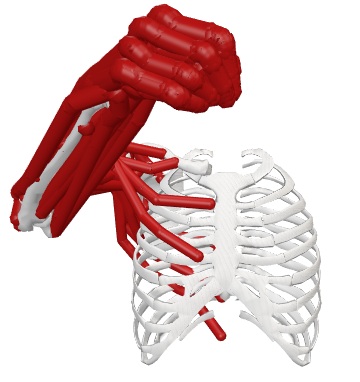
\includegraphics[trim={0 0 0 0}, clip, width=0.7\linewidth]{img/chapter_4/pose_2_front.png}
    \end{minipage}
    \hfill
    \begin{minipage}{0.3\linewidth}
        \captionsetup{justification=centering}
        \centering
        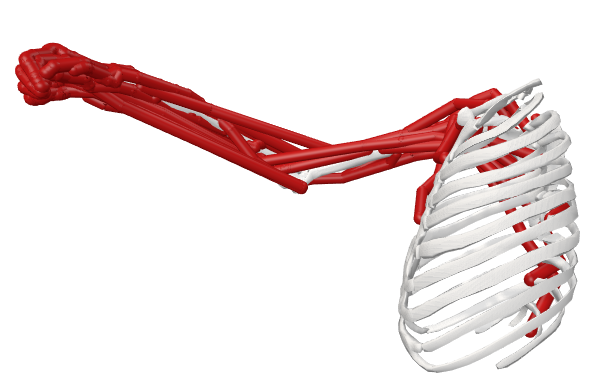
\includegraphics[trim={0 0 0 0}, clip, width=1\linewidth]{img/chapter_4/pose_2_side.png}
    \end{minipage}
    \caption{Fitting posture $\mathbf{q}_6^{\text{fit}}$.}
    \label{fig:pose_6}
\end{figure}

\clearpage
\begin{figure}[!htb]
    \centering
    \captionsetup{justification=centering}
    \begin{minipage}{\linewidth}
        \centering
        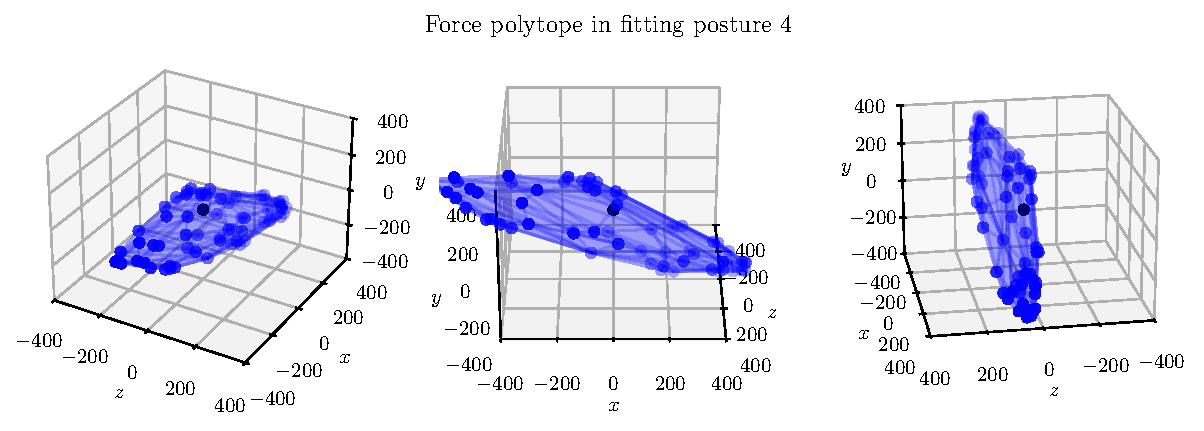
\includegraphics[trim={0 0 0 0}, clip, width=1\linewidth]{img/chapter_4/reconstruction_stanford_imgs/STANFORD_POSTURE_FITTING_04.pdf}
    \end{minipage}
    \caption{Force polytope of the musculoskeletal model parametrized by Stanford's default muscle values in fitting posture $\mathbf{q}_4^{\text{fit}}$. Units are in Newton.}
    \label{fig:polytope_pose_4}
\end{figure}

\begin{figure}[!htb]
    \centering
    \captionsetup{justification=centering}
    \begin{minipage}{\linewidth}
        \centering
        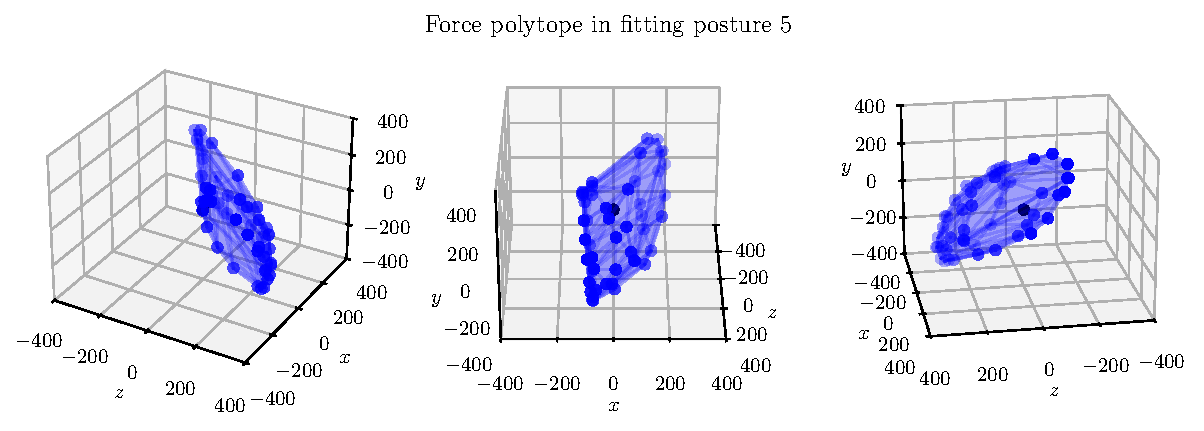
\includegraphics[trim={0 0 0 0}, clip, width=1\linewidth]{img/chapter_4/reconstruction_stanford_imgs/STANFORD_POSTURE_FITTING_05.pdf}
    \end{minipage}
    \caption{Force polytope of the musculoskeletal model parametrized by Stanford's default muscle values in fitting posture $\mathbf{q}_5^{\text{fit}}$. Units are in Newton.}
    \label{fig:polytope_pose_5}
\end{figure}

\begin{figure}[!htb]
    \centering
    \captionsetup{justification=centering}
    \begin{minipage}{\linewidth}
        \centering
        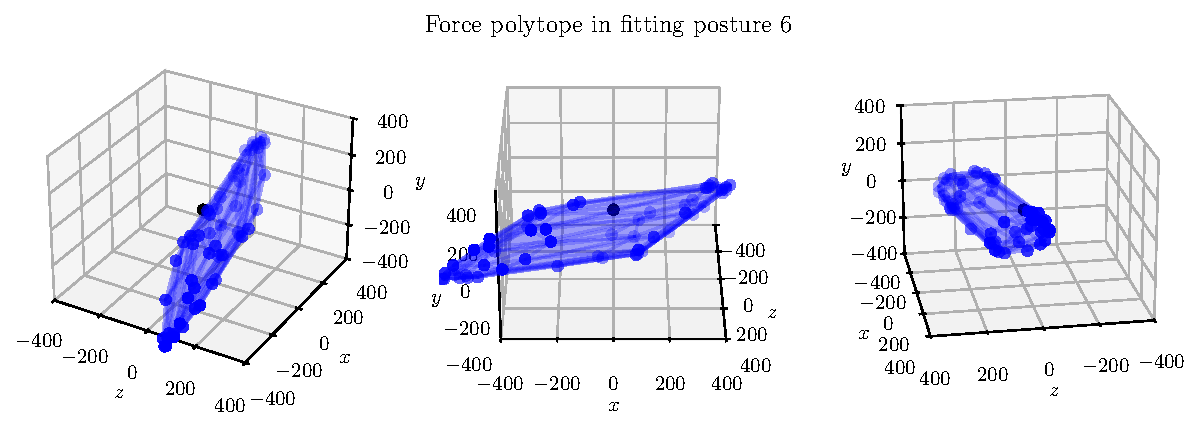
\includegraphics[trim={0 0 0 0}, clip, width=1\linewidth]{img/chapter_4/reconstruction_stanford_imgs/STANFORD_POSTURE_FITTING_06.pdf}
    \end{minipage}
    \caption{Force polytope of the musculoskeletal model parametrized by Stanford's default muscle values in fitting posture $\mathbf{q}_6^{\text{fit}}$. Units are in Newton.}
    \label{fig:polytope_pose_6}
\end{figure}

\clearpage
\paragraph*{Search space size.} For a set of considered muscle parameters, three search spaces are defined and respectively termed \emph{large}, \emph{medium} and \emph{small}. We shall describe them explicitly as intervals for each muscle parameter type considered.

In Stanford's musculoskeletal model, each muscle $M$ force-generating parameter is described by default values noted $f_{iso}^M$ for the maximal isometric force of muscle $M$, $l_o^M$ for the optimal fiber length, $l_s^M$ for the tendon slack length and $\alpha^M$ for the pennation angle. For the muscle geometry, we consider $k > 2$ points in the muscle path (with $\max{k}$ varying from $2$ to $9$ depending on the muscle geometric complexity). The $k$-th point in muscle $M$ is denoted $p_k^M \in \IR^3$. The notation $p_k^M + c$, for $c$ a positive real value, correspond to adding $c$ to each coordinates of the point $p_k^M$. Based on this notation, we define the three search spaces - depending on the muscle parameter type considered in the optimization process - as follows:

\paragraph*{\underline{Large search space:}}
\begin{itemize}[noitemsep]
    \item {\textbf{Maximal isometric force:} (in N): $[f_{iso}^M - 300,\, f_{iso}^M + 300]$;}
    \item {\textbf{Optimal fiber length} (in mm): $[l_o^M - 30,\, l_o^M + 30]$;}
    \item {\textbf{Tendon slack length} (in mm): $[l_o^M - 30,\, l_s^M + 30]$;}
    \item {\textbf{Pennation angle} (in degrees): $[\alpha^M - 20,\, \alpha^M + 20]$;}
    \item {\textbf{Muscle path point} (in mm): $[p_k^M - 10,\, p_k^M + 10]$;}
\end{itemize}

\paragraph*{\underline{Medium search space:}}
\begin{itemize}[noitemsep]
    \item {\textbf{Maximal isometric force:} (in N): $[f_{iso}^M - 200,\, f_{iso}^M + 200]$;}
    \item {\textbf{Optimal fiber length} (in mm): $[l_o^M - 20,\, l_o^M + 20]$;}
    \item {\textbf{Tendon slack length} (in mm): $[l_o^M - 20,\, l_s^M + 20]$;}
    \item {\textbf{Pennation angle} (in degrees): $[\alpha^M - 10,\, \alpha^M + 10]$;}
    \item {\textbf{Muscle path point} (in mm): $[p_k^M - 5,\, p_k^M + 5]$;}
\end{itemize}

\paragraph*{\underline{Small search space:}}
\begin{itemize}[noitemsep]
    \item {\textbf{Maximal isometric force:} (in N): $[f_{iso}^M - 100,\, f_{iso}^M + 100]$;}
    \item {\textbf{Optimal fiber length} (in mm): $[l_o^M - 10,\, l_o^M + 10]$;}
    \item {\textbf{Tendon slack length} (in mm): $[l_o^M - 10,\, l_s^M + 10]$;}
    \item {\textbf{Pennation angle} (in degrees): $[\alpha^M - 5,\, \alpha^M + 5]$;}
    \item {\textbf{Muscle path point} (in mm): $[p_k^M - 1,\, p_k^M + 1]$;}
\end{itemize}

The search spaces defined above are centered around the expected parameter values to find. This is crucial for interpreting the convergence behavior of the optimization algorithms, as both solvers initialize with populations of solutions drawn uniformly within the search space, and do not explicitly evaluates the search space center. This allows us to assess differences in convergence between the genetic algorithm and RACOS. As the results will demonstrate, the genetic algorithm tends to find solutions with parameters located near the search space boundaries, while RACOS generally converges closer to the expected solution, albeit with a lower average objective function value.

% The selected hyperparameters address specific research questions:

%     Which force feasible set representation yields better solutions for predicting force generation in different postures?
%     Which optimization approach effectively identifies solutions within this problem domain?
%     Does the limited number of postures significantly impact solver convergence?
%     Which parameters most strongly influence force feasible set variations?
%     To what extent can muscle parameters be personalized?

This hyperparameter study, conducted within an in silico muscle personalization experiment, aims to determine the feasibility of a set-theoretic approach to maximal force exertion within an optimization framework for muscle personalization. By analyzing the results, we can quantify the irregularity of the objective function's null space, a characteristic hinted at by the complex geometric processes (projection-intersection) involved in generating force feasible sets.

It is relevant to argue on why an hyperparameters study is of interest instead of a traditional sensitivity analysis, which perturbs individual parameters to assess their impact on the output. Our objective necessitates a set-theoretic approach, considering the \emph{combined} influence of all muscle parameters on force production. While the objective function takes a vector of parameters as input (due to the inherent challenges in handling set-valued inputs), this work fundamentally explores how the combined action of muscles, represented as a set of parameters, determines force feasible sets. As a consequence, it is not suitable to consider the impact of the variations of only one muscle parameter over a produced force feasible set. At least a specific type of parameter for \emph{all} muscles should be considered, and this is what is studied in when considering all maximal isometric force, all optimal fiber length, etc. This approach contrasts with traditional sensitivity analysis, which focuses on individual parameter perturbations, but is more suited to our specific set-theoretic case of force feasible production.

In this regard, this hyperparameters study, included in an in silico muscle personalization experiment, seeks to quantity how optimization techniques are suitable for muscle personalization when considering force feasible sets.

\subsection{Validation postures} 
To evaluate how a found solution can generalizes \emph{i.e.} produce expected force feasible sets in other postures, we define $4$ \emph{validation postures} denoted $\mathbf{q}_1^{\text{val}}$, $\mathbf{q}_2^{\text{val}}$, $\mathbf{q}_3^{\text{val}}$ and $\mathbf{q}_4^{\text{val}}$. We denote $\mathcal{Q}^{\text{val}} = \left\{\mathbf{q}_1^{\text{val}}, \mathbf{q}_2^{\text{val}}, \mathbf{q}_3^{\text{val}}, \mathbf{q}_4^{\text{val}}\right\}$ the set of validation postures.

Those postures were chosen qualitatively in regard to how different they are from the previously defined fitting postures.

Table \ref{tab:postures_val_value} summarizes the chosen joint configurations for each of these postures:

\begin{table}[!ht]
    \centering
    \begin{tabular}{|c||c|c|c|c|c|c|c|}
    \hline
    \textbf{Posture} & \makecell{\textbf{Elev} \\ \textbf{angle}} & \makecell{\textbf{Shoulder} \\ \textbf{elevation}} & \makecell{\textbf{Shoulder} \\ \textbf{rotation}} & \makecell{\textbf{Elbow} \\ \textbf{flexion}} & \makecell{\textbf{Pro} \\ \textbf{sup}} & \makecell{\textbf{Wrist} \\ \textbf{deviation}} & \makecell{\textbf{Wrist} \\ \textbf{flexion}} \\
    \hline
    $\mathbf{q}_1^{val}$ & $86$° & $42$° & $98$° & $81$° & $-35$° & $-0.042$ & $-0.200$ \\
    $\mathbf{q}_2^{val}$ & $31$° & $76$° & $28$° & $52$° & $1$° & $0.042$ & $-0.632$ \\
    $\mathbf{q}_3^{val}$ & $63$° & $40$° & $2$° & $53$° & $-1$° & $0.076$ & $0.431$ \\
    $\mathbf{q}_4^{val}$ & $96$° & $74$° & $76$° & $50$° & $0$° & $-0.074$ & $0.216$ \\
    \hline
    \end{tabular}
    \caption{Validation postures parametrization for the validation posture set $\mathcal{Q}_6^{\text{val}} = \left\{\mathbf{q}_1^{\text{val}}, \mathbf{q}_2^{\text{val}}, \mathbf{q}_3^{\text{val}}, \mathbf{q}_4^{\text{val}}\right\}$.}
    \label{tab:postures_val_value}
\end{table}

The following figures show the validation postures in the above-mentionned order.

\begin{figure}[!htb]
    \centering
    \captionsetup{justification=centering}
    \begin{minipage}{0.3\linewidth}
        \centering
        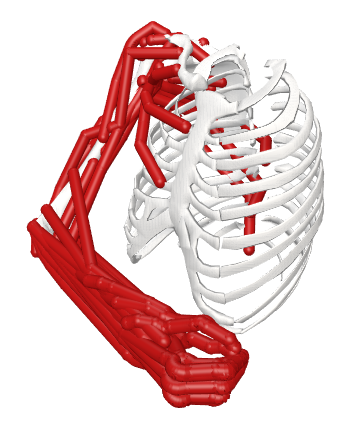
\includegraphics[trim={0 0 0 0}, clip, width=0.6\linewidth]{img/chapter_4/pose_5_view.png}
    \end{minipage}
    \hfill
    \begin{minipage}{0.3\linewidth}
        \captionsetup{justification=centering}
        \centering
        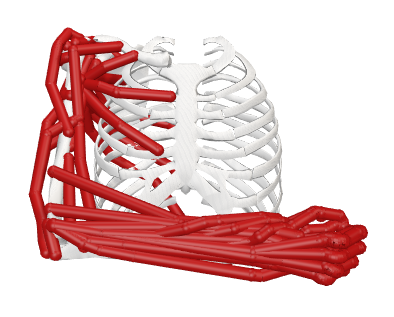
\includegraphics[trim={0 0 0 0}, clip, width=0.8\linewidth]{img/chapter_4/pose_5_front.png}
    \end{minipage}
    \hfill
    \begin{minipage}{0.3\linewidth}
        \captionsetup{justification=centering}
        \centering
        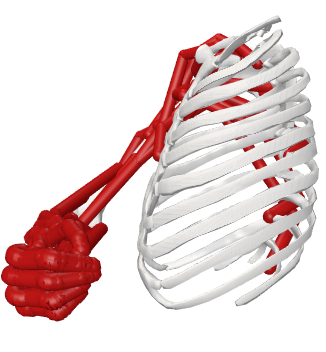
\includegraphics[trim={0 0 0 0}, clip, width=0.6\linewidth]{img/chapter_4/pose_5_side.png}
    \end{minipage}
    \caption{Validation posture $\mathbf{q}_1^{\text{val}}$.}
    \label{fig:pose_val_1}
\end{figure}

\begin{figure}[!htb]
    \centering
    \captionsetup{justification=centering}
    \begin{minipage}{0.35\linewidth}
        \centering
        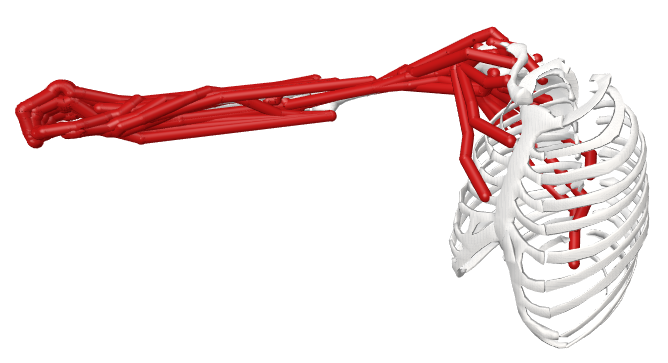
\includegraphics[trim={0 0 0 0}, clip, width=0.9\linewidth]{img/chapter_4/pose_7_view.png}
    \end{minipage}
    \hfill
    \begin{minipage}{0.35\linewidth}
        \captionsetup{justification=centering}
        \centering
        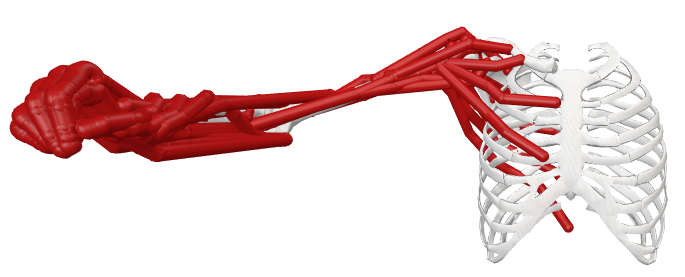
\includegraphics[trim={0 0 0 0}, clip, width=1\linewidth]{img/chapter_4/pose_7_front.png}
    \end{minipage}
    \hfill
    \begin{minipage}{0.25\linewidth}
        \captionsetup{justification=centering}
        \centering
        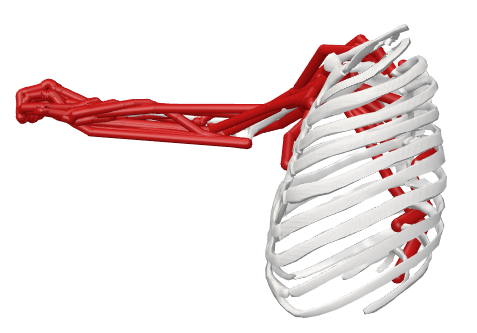
\includegraphics[trim={0 0 0 0}, clip, width=0.9\linewidth]{img/chapter_4/pose_7_side.png}
    \end{minipage}
    \caption{Validation posture $\mathbf{q}_2^{\text{val}}$.}
    \label{fig:pose_val_2}
\end{figure}

\begin{figure}[!htb]
    \centering
    \captionsetup{justification=centering}
    \begin{minipage}{0.35\linewidth}
        \centering
        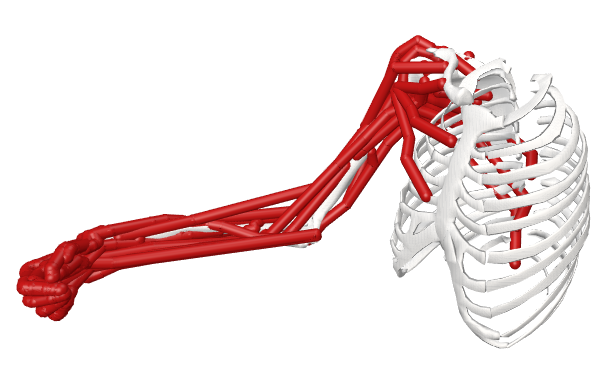
\includegraphics[trim={0 0 0 0}, clip, width=0.9\linewidth]{img/chapter_4/pose_8_view.png}
    \end{minipage}
    \hfill
    \begin{minipage}{0.35\linewidth}
        \captionsetup{justification=centering}
        \centering
        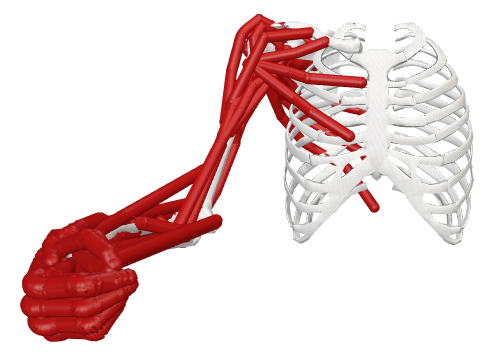
\includegraphics[trim={0 0 0 0}, clip, width=0.8\linewidth]{img/chapter_4/pose_8_front.png}
    \end{minipage}
    \hfill
    \begin{minipage}{0.25\linewidth}
        \captionsetup{justification=centering}
        \centering
        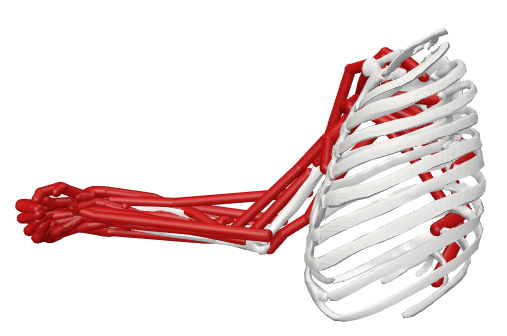
\includegraphics[trim={0 0 0 0}, clip, width=1\linewidth]{img/chapter_4/pose_8_side.png}
    \end{minipage}
    \caption{Validation posture $\mathbf{q}_3^{\text{val}}$.}
    \label{fig:pose_val_3}
\end{figure}

\begin{figure}[!htb]
    \centering
    \captionsetup{justification=centering}
    \begin{minipage}{0.3\linewidth}
        \centering
        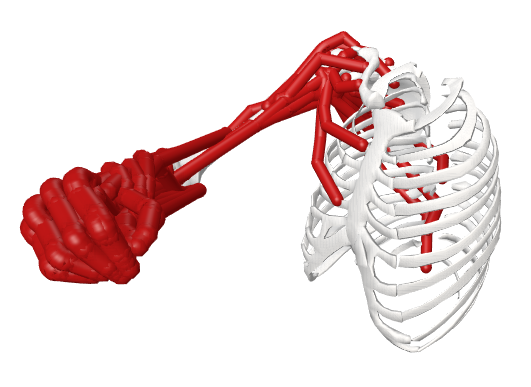
\includegraphics[trim={0 0 0 0}, clip, width=0.8\linewidth]{img/chapter_4/pose_10_view.png}
    \end{minipage}
    \hfill
    \begin{minipage}{0.3\linewidth}
        \captionsetup{justification=centering}
        \centering
        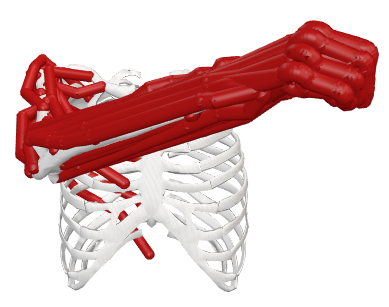
\includegraphics[trim={0 0 0 0}, clip, width=0.8\linewidth]{img/chapter_4/pose_10_front.png}
    \end{minipage}
    \hfill
    \begin{minipage}{0.3\linewidth}
        \captionsetup{justification=centering}
        \centering
        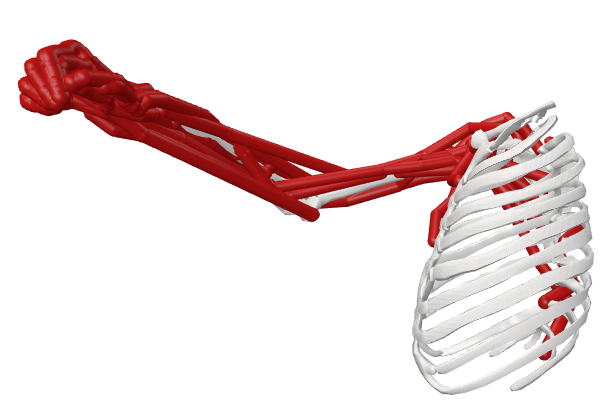
\includegraphics[trim={0 0 0 0}, clip, width=0.9\linewidth]{img/chapter_4/pose_10_side.png}
    \end{minipage}
    \caption{Validation posture $\mathbf{q}_4^{\text{val}}$.}
    \label{fig:pose_val_4}
\end{figure}

Similarly to the fitting postures, the following figures show the force polytopes computed in their respective validation postures.

\begin{figure}[!htb]
    \centering
    \captionsetup{justification=centering}
    \begin{minipage}{\linewidth}
        \centering
        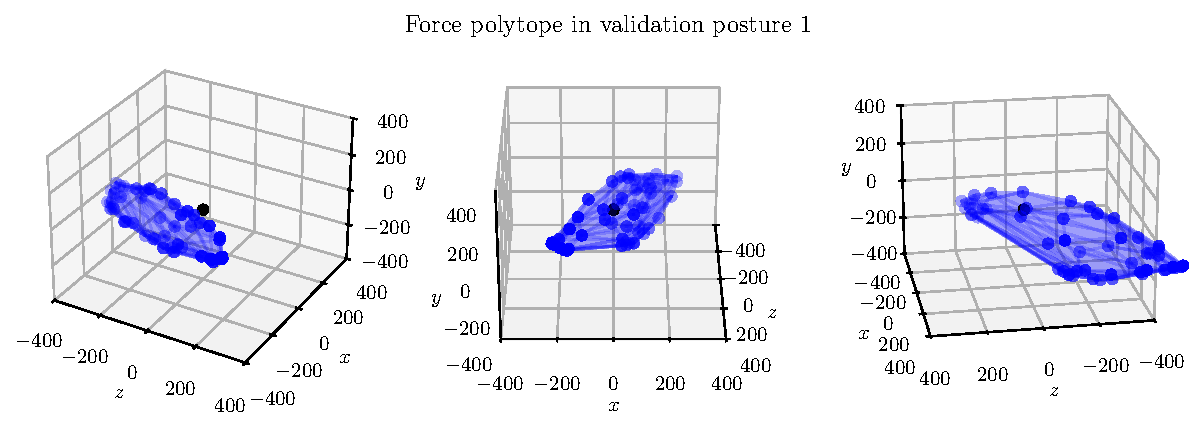
\includegraphics[trim={0 0 0 0}, clip, width=1\linewidth]{img/chapter_4/reconstruction_stanford_imgs/STANFORD_POSTURE_VAL_01.pdf}
    \end{minipage}
    \caption{Force polytope of the musculoskeletal model parametrized by Stanford's default muscle values in validation posture $\mathbf{q}_1^{\text{val}}$. Units are in Newton.}
    \label{fig:polytope_val_pose_1}
\end{figure}

\begin{figure}[!htb]
    \centering
    \captionsetup{justification=centering}
    \begin{minipage}{\linewidth}
        \centering
        \includegraphics[trim={0 0 0 0}, clip, width=1\linewidth]{img/chapter_4/reconstruction_stanford_imgs/STANFORD_POSTURE_VAL_02.pdf}
    \end{minipage}
    \caption{Force polytope of the musculoskeletal model parametrized by Stanford's default muscle values in validation posture $\mathbf{q}_2^{\text{val}}$. Units are in Newton.}
    \label{fig:polytope_val_pose_2}
\end{figure}

\begin{figure}[!htb]
    \centering
    \captionsetup{justification=centering}
    \begin{minipage}{\linewidth}
        \centering
        \includegraphics[trim={0 0 0 0}, clip, width=1\linewidth]{img/chapter_4/reconstruction_stanford_imgs/STANFORD_POSTURE_VAL_03.pdf}
    \end{minipage}
    \caption{Force polytope of the musculoskeletal model parametrized by Stanford's default muscle values in validation posture $\mathbf{q}_3^{\text{val}}$. Units are in Newton.}
    \label{fig:polytope_val_pose_3}
\end{figure}

\begin{figure}[!htb]
    \centering
    \captionsetup{justification=centering}
    \begin{minipage}{\linewidth}
        \centering
        \includegraphics[trim={0 0 0 0}, clip, width=1\linewidth]{img/chapter_4/reconstruction_stanford_imgs/STANFORD_POSTURE_VAL_04.pdf}
    \end{minipage}
    \caption{Force polytope of the musculoskeletal model parametrized by Stanford's default muscle values in validation posture $\mathbf{q}_4^{\text{val}}$. Units are in Newton.}
    \label{fig:polytope_val_pose_4}
\end{figure}

\subsection{Experimental testbed}
The following paragraphs details how the quality of a solution (fitting and validation \emph{accuracy} of its produced force feasible sets) can be evaluated in regard to the hyperparameters. Then, details are mentionned about implemented strategies concerning the time-consuming problematics of computing force polytopes and the repetability of the experiment.

\subsubsection*{Computing accuracy}
For given hyperparameters, the quality of the found solution has to be evaluated. We shall concentrate on studying how close the produced force feasible set $\mathcal{F}_X^{\mathcal{T}}(\mathbf{q}, \theta)$ of a solution $\theta$ in a posture $\mathbf{q}$ is to the expected one $\hat{\mathcal{F}}_X^{\mathcal{T}}(\mathbf{q})$. This computation is done via the comparison function evaluation $d(\hat{\mathcal{F}}_X^{\mathcal{T}}(\mathbf{q}), \, \mathcal{F}_X^{\mathcal{T}}(\mathbf{q}, \theta))$, where $d$ is the comparison function on the discretized version of the force feasible sets defined in \ref{sec:musculoskeletal_model_muscle_pers_sec} and its definition varies according to $\mathcal{T}$.

Two cases are considered: first, we compute the \emph{fitting accuracy}, which describes how close the solution force feasible sets are to the expected ones for the postures used in the objective function. This tells us if the found solution can at least reproduce them. In a second time, the \emph{validation accuracy} describes how the solution can produce force feasible sets in other postures. This helps us to gauge the predictability of the solution.

In complement, another type of accuracy is also considered and directly references the parameter values of the found solution. This allows to gauge the convergence of the used solving algorithms and also to gauge the complexity of the search space.

\subsubsection*{Implementation}
When considering force polytopes as the computed in silico force feasible sets, a total of $420$ optimization processes have been launched using Python. The following paragraphs describe how the implementation was done.

\paragraph*{Force polytope computation.}
When the force feasible set are computed in silico using a tension set model $\mathcal{T}_{\infty}$ (a hyperrectangle of dimension $50$), the produced force feasible set is a 3-dimensional polytope. As described in chapter \ref{chapter:2}, a set of points on their surface can be computed using Skuric et al. Iterative Convex Hull (ICH) algorithm (\cite{skuricOnLineFeasibleWrench2022}). The quality of this approximation depends on a tolerance parameter, which describe the maximal distance between a bounding hyperplane of the approximated polytope and an expected vertex. In this experimental testbed, a tolerance value of $5$ Newton is chosen. While it could have been chosen to be lower, $5$ N allows a tradeoff between the quality of the approximation and the computation time.

It should be noted that a solution may produce non-computable force feasible sets, meaning that the torque feasible set does not intersect with the image of the Jacobian transpose. It was observed empirically that this phenomenom arises most of the time with a random solution in a large search space. Also, the more parameters are to be optimized on, the more infeasible solutions there seem to be. It will be shown that genetic algorithms suffer from this but RACOS does not, as its underlying probabilistic model learns where to not search as well. In these cases, any used objective function with a non-computable force feasible sets is set to evaluate at $+\infty$. 

\paragraph*{Repetability.} To evaluate if a solving method is \emph{repetable}, \emph{i.e.} the found solution quality or the convergence of the algorithm are not fortunate coincidences of the randomly generated set of initial solutions, the optimization process must be solved using different initial solutions. As such, all scripts have been relaunched $5$ times. 

\paragraph*{Leveraging the optimization time process.}
As the evaluation of the objective function is expensive in time and the optimization is done a high-dimensional search-space, only one script could take about $4$ hours to complete. To account for the large amount of hyperparameters as well as the $5$ repetitions for each of them, all optimizations have been launched in parallel (one script per core) on several machines. Each of these machines features 2x32-core AMD Zen2 EPYC 7452 CPUs cadenced at 2.35 GHz.

For further contributions to this in silico tests, we ensured that most machines could run the scripts. Indeed, the processor type (Intel, AMD, ARM, etc.) influences the time computation of force polytopes with ICH algorithm, as it requires linear algebra tasks for computing approximated vertices. This is mainly due to the underlying matrix computations implementation available on a machine. We used OpenBLAS (\cite{wangAUGEMAutomaticallyGenerate2013}) as it is open-source and available for a significant amount of processor architectures.

% \paragraph*{}

% \clearpage
\subsection{Results}
This section analyzes the optimization results across all trials with specified hyperparameters. To assess the quality of the resulting polytopic sets, the discretized distance metric (defined in Section \ref{sec:musculoskeletal_model_muscle_pers_sec}) is employed. Interpretation of this metric requires considering the following empirically derived distance values $d$ with associated qualitative bounds defined as:

% This section focuses on presenting the results of the optimization processes for all trials in given hyperparameters. We present the results then interpret in details. In order to qualitatively appreciate the results, mostly described using the discretized distance defined in \ref{sec:musculoskeletal_model_muscle_pers_sec}, its evaluation values have to be interpreted with care as we are dealing with polytopic sets. We found empiric distance values allowing us to weight the distance meaning: when two compared polytopes have a discretized distance $d$, then the following empiric rules have been defined according to bound values. These bounds are not strict, and have been drawn from the produced force polytopes considered in the specific chosen postures:

\begin{itemize}[noitemsep]
    \item {$d<10$: the polytopes' surfaces almost coincide, sharing a similar face structure and the same number of vertices. (Fig. \ref{fig:polytope_racos_p6_pen_small_output_3207074_trial_3_fitting_posture_5});}
    \item {$10<d<50$: the polytopes consistently exhibit similar shapes, elongation, and orientation. They may slightly overlap or be nested (one polytope is contained within another) (Fig. \ref{fig:polytope_racos_p3_opt_medium_output_3205633_trial_5_fitting_posture_1});}
    \item {$50 < d < 100$: the polytopes exhibit four types of spatial differences: in translation, scaling and slight rotations as in figure \ref{fig:polytope_racos_p6_tsl_medium_output_3207082_trial_1_fitting_posture_1}, but also nesting. Nesting is particularly difficult to identify visually, as shown in figure \ref{fig:polytope_genetic_p6_pen_large_output_3215217_trial_4_fitting_posture_5};}
    \item {$d >100$: the polytopes' elongation, orientation, scaling, shape and offset vary considerably (Fig. \ref{fig:polytope_racos_p6_points_medium_output_3207004_trial_5_fitting_posture_3})}
\end{itemize}

These bounds, derived from force polytopes generated in specific postures, provide a framework for evaluating the relative similarity of the optimized polytopes.
They have been concluded from qualitative appreciation of force polytopes produced by \emph{all} the solutions found after an optimization processes. The reader is invited to also appreciate these distances\footnote{\url{https://gitlab.inria.fr/auctus-team/people/gautierlaisne/public/reconstruction_stanford}}, in the folder dedicated to each force polytopes images of the solutions.

Although not a formally derived result, the qualitative observation that the discretized distance reflects global polytope shape is noteworthy. This correlation, however, arises from the specific geometric construction of force polytopes and the relatively narrow considered search spaces (in the sense that all search spaces do not have a range in a higher order of magnitude than its center). This anaysis should not be generalized to arbitrary polytopes.

% \clearpage
\begin{figure}[!htb]
    \centering
    \captionsetup{justification=centering}
    
    \begin{minipage}{0.8\linewidth}
        \captionsetup{justification=centering}
        \centering
        \includegraphics[trim={0 0 0 0}, clip, width=1\linewidth]{img/chapter_4/reconstruction_stanford_imgs/polytope_racos_p6_pen_small_output_3207074_trial_3_fitting_posture_5.pdf}
    \end{minipage}
    \begin{minipage}{0.8\linewidth}
        \captionsetup{justification=centering}
        \centering
        \includegraphics[trim={0 0 0 20}, clip, width=1\linewidth]{img/chapter_4/reconstruction_stanford_imgs/polytope_racos_p6_pen_small_output_3207074_trial_3_fitting_posture_5_with_stanford.pdf}
    \end{minipage}
    \caption{Comparison in fitting posture 5 of reference force polytope (second row, in blue) and the force polytope produced the best solution (in cost) found from the third run of pennation angle parameter type optimizations, configured with hyperparameters: RACOS solver, small search space, posture set $\mathcal{Q}_6^{\text{fit}}$. Its cost is of $5$ Newton in this posture.}
    \label{fig:polytope_racos_p6_pen_small_output_3207074_trial_3_fitting_posture_5}
\end{figure}


\begin{figure}[!htb]
    \centering
    \captionsetup{justification=centering}
    
    \begin{minipage}{0.8\linewidth}
        \captionsetup{justification=centering}
        \centering
        \includegraphics[trim={0 0 0 0}, clip, width=1\linewidth]{img/chapter_4/reconstruction_stanford_imgs/polytope_racos_p3_opt_medium_output_3205633_trial_5_fitting_posture_1.pdf}
    \end{minipage}
    \begin{minipage}{0.8\linewidth}
        \captionsetup{justification=centering}
        \centering
        \includegraphics[trim={0 0 0 20}, clip, width=1\linewidth]{img/chapter_4/reconstruction_stanford_imgs/polytope_racos_p3_opt_medium_output_3205633_trial_5_fitting_posture_1_with_stanford.pdf}
    \end{minipage}
    \caption{Comparison in fitting posture 1 of reference force polytope (second row, in blue) and the force polytope produced the best solution (in cost) found from the first run of optimal fiber length parameter type optimizations, configured with hyperparameters: RACOS solver, medium search space, posture set $\mathcal{Q}_3^{\text{fit}}$. Its cost is of $38$ Newton in this posture.}
    \label{fig:polytope_racos_p3_opt_medium_output_3205633_trial_5_fitting_posture_1}
\end{figure}

\clearpage
\begin{figure}[!htb]
    \centering
    \captionsetup{justification=centering}
    
    \begin{minipage}{0.8\linewidth}
        \captionsetup{justification=centering}
        \centering
        \includegraphics[trim={0 0 0 0}, clip, width=1\linewidth]{img/chapter_4/reconstruction_stanford_imgs/polytope_racos_p6_tsl_medium_output_3207082_trial_1_fitting_posture_1.pdf}
    \end{minipage}
    \begin{minipage}{0.8\linewidth}
        \captionsetup{justification=centering}
        \centering
        \includegraphics[trim={0 0 0 20}, clip, width=1\linewidth]{img/chapter_4/reconstruction_stanford_imgs/polytope_racos_p6_tsl_medium_output_3207082_trial_1_fitting_posture_1_with_stanford.pdf}
    \end{minipage}
    \caption{Comparison in fitting posture 1 of reference force polytope (second row, in blue) and the force polytope produced the best solution (in cost) found from the first run of tendon slack length parameter type optimizations, configured with hyperparameters: RACOS solver, medium search space, posture set $\mathcal{Q}_6^{\text{fit}}$. Its cost is of $94$ Newton in this posture.}
    \label{fig:polytope_racos_p6_tsl_medium_output_3207082_trial_1_fitting_posture_1}
\end{figure}

\begin{figure}[!htb]
    \centering
    \captionsetup{justification=centering}
    
    \begin{minipage}{0.8\linewidth}
        \captionsetup{justification=centering}
        \centering
        \includegraphics[trim={0 0 0 0}, clip, width=1\linewidth]{img/chapter_4/reconstruction_stanford_imgs/polytope_racos_p6_points_medium_output_3207004_trial_5_fitting_posture_3.pdf}
    \end{minipage}
    \begin{minipage}{0.8\linewidth}
        \captionsetup{justification=centering}
        \centering
        \includegraphics[trim={0 0 0 20}, clip, width=1\linewidth]{img/chapter_4/reconstruction_stanford_imgs/polytope_racos_p6_points_medium_output_3207004_trial_5_fitting_posture_3_with_stanford.pdf}
    \end{minipage}
    \caption{Comparison in fitting posture 3 of reference force polytope (second row, in blue) and the force polytope produced the best solution (in cost) found from the fifth run of muscle geometry parameter type optimizations, configured with hyperparameters: RACOS solver, medium search space, posture set $\mathcal{Q}_6^{\text{fit}}$. Its cost is of $119$ Newton in this posture.}
    \label{fig:polytope_racos_p6_points_medium_output_3207004_trial_5_fitting_posture_3}
\end{figure}

\clearpage
\subsubsection*{Accuracy of computed polytopes in the fitting postures}

Three tables summarize the discretized distance of the force polytopes generated by the best solutions for each set of hyperparameters. Table \ref{tab:accuracy_fitting_pol_MEAN_COST_FCT_OVER_ALL_SOLUTIONS} contains the average (and standard deviation) of the cost function evaluated for each of the best solution found of the $5$ trials per given hyperparameters. Since the cost function corresponds to the maximum distance between a predicted polytope in a certain posture and the polytope to attaign, averaging over the $5$ trials is interpretable as the \emph{mean worst case discretized distance} over all considered postures.

\bgroup
\def\arraystretch{1.2}
\begin{table}[!ht]
    \scriptsize
    \centering
    \begin{tabular}{|c|c|c|c|c|c|c|c|c|c|}
    \hline
    \multirow{4}{*}{\makecell{\textbf{Fitting} \\ \textbf{posture} \\ \textbf{set}}} & 
    \multirow{4}{*}{\makecell{\textbf{Solver}}} & 
    \multirow{4}{*}{\makecell{\textbf{Search} \\ \textbf{space} \\ \textbf{size}}} & 
    \multicolumn{7}{c|}{\makecell{\textbf{Parameter type}}} \\
    \cline{4-10}

    & & & \makecell{$f_{iso}$} & \makecell{$l_o$} & \makecell{$l_s$} & \makecell{$\alpha$} & \makecell{$f_{iso}$, $l_o$, $l_s$} & \makecell{Muscle \\geometry} & \makecell{$f_{iso}$, $l_o$, $l_s$ \\ + muscle \\ geometry} \\
    % \hline
    \hline
    \multirow{6}{*}{\makecell{Posture set \\ $\mathcal{Q}_3^{\text{fit}}$}} & \multirow{3}{*}{\makecell{RACOS}} 
      & \makecell{Large} &  $61\pm 11$ & $93\pm 15$ & $63\pm 18$ & $16\pm 2$ & $101\pm 19$ & $101\pm 20$ & $113\pm 25$ \\  \cline{3-10}
    & & \makecell{Medium} & $49\pm 7$ & $56\pm 17$ & $60\pm 12$ & $11\pm 1$ & $74\pm 7$ & $50\pm 12$ & $86\pm 8$ \\  \cline{3-10}
    & & \makecell{Small} &  $42\pm 6$ & $39\pm 7$ & $34\pm 6$ & $5\pm 2$ & $57\pm 6$ & $19\pm 5$ & $55\pm 15$ \\ 
    \cline{2-10}

    & \multirow{3}{*}{\makecell{GA}} 
      & \makecell{Large} &  $137\pm 19$ & $341\pm 181$ & $139\pm 5$ & $67\pm 4$ & $181\pm 13$ & $365\pm 83$ & $*$ \\  \cline{3-10}
    & & \makecell{Medium} & $116\pm 10$ & $122\pm 12$ & $126\pm 11$ & $42\pm 4$ & $157\pm 14$ & $119\pm 12$ & $*$ \\  \cline{3-10}
    & & \makecell{Small} &  $96\pm 6$ & $118\pm 5$ & $108\pm 9$ & $35\pm 2$ & $103\pm 5$ & $61\pm 2$ & $*$ \\ 
    \hline
    \hline
    \multirow{6}{*}{\makecell{Posture set \\ $\mathcal{Q}_6^{\text{fit}}$}} & \multirow{3}{*}{\makecell{RACOS}} 
      & \makecell{Large} &  $117\pm 12$ & $143\pm 17$ & $115\pm 13$ & $33\pm 7$ & $135\pm 32$ & $138\pm 17$ & $149\pm 12$ \\  \cline{3-10}
    & & \makecell{Medium} & $92\pm 18$ & $100\pm 24$ & $86\pm 13$ & $22\pm 1$ & $109\pm 14$ & $113\pm 7$ & $131\pm 5$ \\  \cline{3-10}
    & & \makecell{Small} &  $63\pm 6$ & $59\pm 10$ & $59\pm 7$ & $16\pm 1$ & $17\pm 12$ & $37\pm 7$ & $90\pm 15$ \\ 
    \cline{2-10}

    & \multirow{3}{*}{\makecell{GA}} 
      & \makecell{Large} &  $181\pm 9$ & $276\pm 48$ & $204\pm 13$ & $84\pm 6$ & $217\pm 13$ & $619\pm 125$ & $*$ \\  \cline{3-10}
    & & \makecell{Medium} & $163\pm 8$ & $174\pm 10$ & $151\pm 8$ & $75\pm 6$ & $178\pm 11$ & $143\pm 9$ & $*$ \\  \cline{3-10}
    & & \makecell{Small} &  $135\pm 5$ & $129\pm 4$ & $125\pm 6$ & $57\pm 1$ & $137\pm 6$ & $117\pm 4$ & $*$ \\ 
    \hline
    
    \end{tabular}
    \caption{For a set of hyperparameters (both expressed as columns and rows), mean and standard deviation (in N) of the cost function evaluated for the best solution for each of the $5$ trials. A $*$ symbol denotes that no solution found over the 5 trials could produce computable force feasible sets. \emph{GA} stands for Genetic Algorithm.}
    \label{tab:accuracy_fitting_pol_MEAN_COST_FCT_OVER_ALL_SOLUTIONS}
\end{table}
\egroup

Tables \ref{tab:accuracy_fitting_pol_p3} and \ref{tab:accuracy_fitting_ellipsoid_p6} provide further comparison between the obtained and expected force polytopes. These tables show the mean and standard deviation (in Newtons, rounded to the nearest unit) of the discretized distance between the expected and obtained polytopes for each posture in $\mathcal{Q}_3^{\text{fit}}$ and $\mathcal{Q}_6^{\text{fit}}$, respectively. These values are calculated across all 5 trials for each combination of hyperparameters, including the solver, search space size, and parameter type (presented in rows and columns). For better readability, separate tables are used for the different posture sets.

\clearpage
\bgroup
\def\arraystretch{1.2}
\begin{table}[!ht]
    \tiny
    \centering
    \begin{tabular}{|c|c|c|c|c|c|c|c|c|c|}
    \hline
    \multirow{4}{*}{\makecell{\textbf{Solver}}} & 
    \multirow{4}{*}{\makecell{\textbf{Search} \\ \textbf{space} \\ \textbf{size}}} &
    \multirow{4}{*}{\makecell{\textbf{Fitting} \\ \textbf{postures}}} & 
    \multicolumn{7}{c|}{\makecell{\textbf{Parameter type}}} \\
    \cline{4-10}

    & & & \makecell{$f_{iso}$} & \makecell{$l_o$} & \makecell{$l_s$} & \makecell{$\alpha$} & \makecell{$f_{iso}$, $l_o$, $l_s$} & \makecell{Muscle \\geometry} & \makecell{$f_{iso}$, $l_o$, $l_s$ \\ + muscle \\ geometry} \\
    % \hline
    \hline
    \multirow{9}{*}{\begin{turn}{90}\makecell{RACOS}\end{turn}} & \multirow{3}{*}{\begin{turn}{90}\makecell{Large}\end{turn}} 
    & $\mathbf{q}_1^{\text{fit}}$ & $60\pm 1$ & $91\pm 16$ & $58\pm 18$ & $16\pm 2$ & $96\pm 24$ & $100\pm 20$ & $112\pm 26$ \\\cline{3-10}
    & & $\mathbf{q}_2^{\text{fit}}$ & $59\pm 13$ & $84\pm 24$ & $58\pm 17$ & $15\pm 2$ & $90\pm 2$ & $98\pm 20$ & $112\pm 26$ \\\cline{3-10}
    & & $\mathbf{q}_3^{\text{fit}}$ & $60\pm 13$ & $81\pm 17$ & $61\pm 18$ & $14\pm 5$ & $100\pm 19$ & $100\pm 20$ & $107\pm 29$ \\\cline{3-10}
    \cline{2-10}
    & \multirow{3}{*}{\begin{turn}{90}\makecell{Medium}\end{turn}} 
    & $\mathbf{q}_1^{\text{fit}}$ & $47\pm 6$ & $51\pm 117$ & $52\pm 15$ & $11\pm 1$ & $71\pm 8$ & $49\pm 13$ & $85\pm 9$ \\\cline{3-10}
    & & $\mathbf{q}_2^{\text{fit}}$ & $46\pm 5$ & $52\pm 16$ & $55\pm 16$ & $9\pm 2$ & $71\pm 9$ & $50\pm 13$ & $84\pm 10$ \\\cline{3-10}
    & & $\mathbf{q}_3^{\text{fit}}$ & $47\pm 7$ & $55\pm 19$ & $59\pm 12$ & $7\pm 3$ & $71\pm 8$ & $50\pm 12$ & $84\pm 1$ \\\cline{3-10}
    \cline{2-10}
    & \multirow{3}{*}{\begin{turn}{90}\makecell{Small}\end{turn}}  
    & $\mathbf{q}_1^{\text{fit}}$ & $41\pm 5$ & $36\pm 6$ & $32\pm 5$ & $5\pm 2$ & $50\pm 6$ & $18\pm 5$ & $53\pm 16$ \\\cline{3-10}
    & & $\mathbf{q}_2^{\text{fit}}$ & $38\pm 4$ & $30\pm 6$ & $33\pm 6$ & $5\pm 2$ & $51\pm 1$ & $18\pm 5$ & $50\pm 13$ \\\cline{3-10}
    & & $\mathbf{q}_3^{\text{fit}}$ & $42\pm 7$ & $39\pm 7$ & $32\pm 8$ & $4\pm 2$ & $55\pm 7$ & $19\pm 5$ & $55\pm 15$ \\\cline{3-10}
    \hline
    \hline
    
    \multirow{9}{*}{\begin{turn}{90}\makecell{GENETIC \\ ALGORITHM}\end{turn}} & \multirow{3}{*}{\begin{turn}{90}\makecell{Large}\end{turn}}  
    & $\mathbf{q}_1^{\text{fit}}$ & $134\pm 49$ & $283\pm 201$ & $132\pm 13$ & $38\pm 9$ & $146\pm 47$ & $246\pm 38$ & $*$ \\\cline{3-10}
    & & $\mathbf{q}_2^{\text{fit}}$ & $117\pm 33$ & $238\pm 104$ & $140\pm 5$ & $42\pm 10$ & $166\pm 26$ & $226\pm 55$ & $*$ \\\cline{3-10}
    & & $\mathbf{q}_3^{\text{fit}}$ & $114\pm 23$ & $284\pm 239$ & $107\pm 15$ & $58\pm 14$ & $160\pm 52$ & $307\pm 117$ & $*$ \\
    \cline{2-10}
    & \multirow{3}{*}{\begin{turn}{90}\makecell{Medium}\end{turn}}  
    & $\mathbf{q}_1^{\text{fit}}$ & $110\pm 31$ & $127\pm 19$ & $109\pm 14$ & $26\pm 10$ & $127\pm 18$ & $104\pm 36$ & $*$ \\\cline{3-10}
    & & $\mathbf{q}_2^{\text{fit}}$ & $95\pm 45$ & $140\pm 33$ & $111\pm 16$ & $30\pm 9$ & $145\pm 69$ & $106\pm 31$ & $*$ \\\cline{3-10}
    & & $\mathbf{q}_3^{\text{fit}}$ & $106\pm 29$ & $116\pm 38$ & $116\pm 3$ & $52\pm 6$ & $116\pm 49$ & $99\pm 22$ & $*$ \\
    \cline{2-10}
    & \multirow{3}{*}{\begin{turn}{90}\makecell{Small}\end{turn}}  
     & $\mathbf{q}_1^{\text{fit}}$ & $93\pm 22$ & $90\pm 26$ & $82\pm 26$ & $19\pm 9$ & $105\pm 22$ & $20\pm 4$ & $*$ \\\cline{3-10}
    & & $\mathbf{q}_2^{\text{fit}}$ & $67\pm 9$ & $81\pm 55$ & $122\pm 27$ & $29\pm 9$ & $114\pm 24$ & $43\pm 24$ & $*$ \\\cline{3-10}
    & & $\mathbf{q}_3^{\text{fit}}$ & $104\pm 22$ & $140\pm 5$ & $127\pm 8$ & $36\pm 16$ & $100\pm 19$ & $59\pm 14$ & $*$ \\
    \hline

    \end{tabular}
    \caption{Rounded mean and standard deviation (in N) of the discretized distance between the produced and expected force polytope in every posture defined in $\mathcal{Q}_3^{\text{fit}}$, for each best solution over the 5 trials.}
    \label{tab:accuracy_fitting_pol_p3}
\end{table}
\egroup

\bgroup
\def\arraystretch{1.2}
\begin{table}[!ht]
    \tiny
    \centering
    \begin{tabular}{|c|c|c|c|c|c|c|c|c|c|}
    \hline
    \multirow{4}{*}{\makecell{\textbf{Solver}}} & 
    \multirow{4}{*}{\makecell{\textbf{Search} \\ \textbf{space} \\ \textbf{size}}} &
    \multirow{4}{*}{\makecell{\textbf{Fitting} \\ \textbf{postures}}} & 
    \multicolumn{7}{c|}{\makecell{\textbf{Parameter type}}} \\
    \cline{4-10}

    & & & \makecell{$f_{iso}$} & \makecell{$l_o$} & \makecell{$l_s$} & \makecell{$\alpha$} & \makecell{$f_{iso}$, $l_o$, $l_s$} & \makecell{Muscle \\geometry} & \makecell{$f_{iso}$, $l_o$, $l_s$ \\ + muscle \\ geometry} \\
    \hline
    % \hline
    \multirow{18}{*}{\begin{turn}{90}\makecell{RACOS}\end{turn}} & \multirow{6}{*}{\begin{turn}{90}\makecell{Large}\end{turn}} 
    & $\mathbf{q}_1^{\text{fit}}$ & $105\pm 24$ & $104\pm 19$ & $92\pm 17$  & $28\pm 9$ & $116\pm 48$ &  $127\pm 18$ & $130\pm 17$ \\
    \cline{3-10}
    & & $\mathbf{q}_2^{\text{fit}}$ & $100\pm 21$ & $116\pm 19$ & $107\pm 13$ & $21\pm 6$ & $161\pm 71$ & $124\pm 24$ & $149\pm 12$ \\
    \cline{3-10}
    & & $\mathbf{q}_3^{\text{fit}}$ & $84\pm 21$ & $111\pm 35$ & $102\pm 24$ & $29\pm 9$ & $134\pm 32$ & $126\pm 28$ & $143\pm 24$ \\
    \cline{3-10}
    & & $\mathbf{q}_4^{\text{fit}}$ & $104\pm 12$ & $137\pm 11$ & $106\pm 9$ & $24\pm 10$ & $126\pm 35$ & $136\pm 20$ & $142\pm 26$ \\
    \cline{3-10}
    & & $\mathbf{q}_5^{\text{fit}}$ & $94\pm 25$ & $135\pm 22$ & $107\pm 16$ & $26\pm 8$ & $131\pm 31$ & $134\pm 17$ & $149\pm 12$ \\
    \cline{3-10}
    & & $\mathbf{q}_6^{\text{fit}}$ & $110\pm 15$ & $116\pm 17$ & $94\pm 15$ & $26\pm 3$ & $154\pm 75$ & $124\pm 22$ & $137\pm 15$ \\
    \cline{2-10}
    & \multirow{6}{*}{\begin{turn}{90}\makecell{Medium}\end{turn}} 
    & $\mathbf{q}_1^{\text{fit}}$ & $74\pm 21$ & $78\pm 22$ &   $75\pm 27$  & $18\pm 3$ & $102\pm 15$ & $110\pm 5$ & $109\pm 24$ \\
    \cline{3-10}
    & & $\mathbf{q}_2^{\text{fit}}$ & $89\pm 18$ & $87\pm 22$ &  $70\pm 20$   & $16\pm 6$ & $91\pm 24$ & $98\pm 24$ & $119\pm 9$ \\
    \cline{3-10}
    & & $\mathbf{q}_3^{\text{fit}}$ & $82\pm 26$ & $95\pm 29$ &  $75\pm 20$  & $19\pm 4$ & $106\pm 17$ & $102\pm 25$ & $126\pm 13$ \\
    \cline{3-10}
    & & $\mathbf{q}_4^{\text{fit}}$ & $86\pm 15$ & $87\pm 17$ & $78\pm 22$   & $19\pm 6$ & $100\pm 16$ & $106\pm 6$ & $130\pm 4$ \\
    \cline{3-10}
    & & $\mathbf{q}_5^{\text{fit}}$ & $85\pm 22$ & $88\pm 21$ &  $83\pm 11$    & $17\pm 2$ & $108\pm 14$ & $107\pm 6$ & $122\pm 13$ \\
    \cline{3-10}
    & & $\mathbf{q}_6^{\text{fit}}$ & $75\pm 18$ & $89\pm 22$ & $75\pm 28$   & $16\pm 4$ & $96\pm 15$ & $88\pm 10$ & $103\pm 25$ \\
    \cline{2-10}
    & \multirow{6}{*}{\begin{turn}{90}\makecell{Small}\end{turn}} 
    & $\mathbf{q}_1^{\text{fit}}$ & $61\pm 8$ & $44\pm 14$ & $43\pm 8$ & $9\pm 4$ & $62\pm 6$ & $22\pm 6$ & $86\pm 13$ \\
    \cline{3-10}
    & & $\mathbf{q}_2^{\text{fit}}$ & $49\pm 10$ & $45\pm 17$ & $54\pm 7$ & $6\pm 2$ & $61\pm 16$ & $30\pm 4$ & $87\pm 17$ \\
    \cline{3-10}
    & & $\mathbf{q}_3^{\text{fit}}$ & $53\pm 5$ & $53\pm 14$ & $54\pm 6$& $15\pm 1$ & $68\pm 12$ & $35\pm 9$ & $74\pm 28$ \\
    \cline{3-10}
    & & $\mathbf{q}_4^{\text{fit}}$ & $56\pm 6$ & $54\pm 9$ & $45\pm 11$ & $12\pm 2$ & $64\pm 12$ & $31\pm 11$ & $87\pm 19$ \\
    \cline{3-10}
    & & $\mathbf{q}_5^{\text{fit}}$ & $46\pm 10$ & $48\pm 15$ & $52\pm 10$ & $4\pm 2$ & $63\pm 17$ & $35\pm 7$ & $82\pm 15$ \\
    \cline{3-10}
    & & $\mathbf{q}_6^{\text{fit}}$ & $55\pm 9$ & $50\pm 10$ & $55\pm 16$ & $12\pm 3$ & $67\pm 18$ & $34\pm 7$ & $79\pm 14$ \\
    \hline
    \hline
    % \cellcolor[HTML]{EBF3FF}$5$ & \cellcolor[HTML]{FFFFD1}
    \multirow{18}{*}{\begin{turn}{90}\makecell{GENETIC ALGORITHM}\end{turn}} & \multirow{6}{*}{\begin{turn}{90}\makecell{Large}\end{turn}} 
    & $\mathbf{q}_1^{\text{fit}}$ & $106\pm 28$ & $221\pm 15$ & $159\pm 28$ & $33\pm 7$ & $141\pm 27$ & $357\pm 137$ & $*$ \\
    \cline{3-10}
    & & $\mathbf{q}_2^{\text{fit}}$ & $132\pm 66$ & $173\pm 104$ & $146\pm 32$ & $54\pm 7$ & $194\pm 72$ & $482\pm 240$ & $*$ \\
    \cline{3-10}
    & & $\mathbf{q}_3^{\text{fit}}$ & $118\pm 22$ & $253\pm 47$ & $147\pm 44$ & $81\pm 15$ & $150\pm 41$ & $432\pm 299$ & $*$ \\
    \cline{3-10}
    & & $\mathbf{q}_4^{\text{fit}}$ & $138\pm 38$ & $180\pm 95$ & $210\pm 20$ & $56\pm 12$ & $189\pm 57$ & $384\pm 119$ & $*$ \\
    \cline{3-10}
    & & $\mathbf{q}_5^{\text{fit}}$ & $180\pm 48$ & $195\pm 71$ & $164\pm 16$ & $73\pm 29$ & $179\pm 16$ & $343\pm 191$ & $*$ \\
    \cline{3-10}
    & & $\mathbf{q}_6^{\text{fit}}$ & $120\pm 14$ & $175\pm 83$ & $173\pm 33$ & $78\pm 24$ & $167\pm 22$ & $422\pm 280$ & $*$ \\
    \cline{2-10}
    & \multirow{6}{*}{\begin{turn}{90}\makecell{Medium}\end{turn}}
    & $\mathbf{q}_1^{\text{fit}}$ & $119\pm 15$ & $138\pm 9$ & $129\pm 11$ & $30\pm 2$ & $138\pm 33$ & $113\pm 19$ & $*$ \\
    \cline{3-10}
    & & $\mathbf{q}_2^{\text{fit}}$ & $110\pm 32$ & $123\pm 16$ & $99\pm 5$ & $33\pm 19$ & $173\pm 46$ & $130\pm 22$ & $*$ \\
    \cline{3-10}
    & & $\mathbf{q}_3^{\text{fit}}$ & $99\pm 16$ & $146\pm 19$ & $120\pm 19$ & $70\pm 8$ & $148\pm 18$ & $91\pm 30$ & $*$ \\
    \cline{3-10}
    & & $\mathbf{q}_4^{\text{fit}}$ & $154\pm 51$ & $219\pm 54$ & $225\pm 27$ & $34\pm 15$ & $163\pm 46$ & $179\pm 46$ & $*$ \\
    \cline{3-10}
    & & $\mathbf{q}_5^{\text{fit}}$ & $174\pm 39$ & $169\pm 42$ & $148\pm 22$ & $68\pm 16$ & $193\pm 53$ & $128\pm 37$ & $*$ \\
    \cline{3-10}
    & & $\mathbf{q}_6^{\text{fit}}$ & $96\pm 20$ & $229\pm 47$ & $119\pm 23$ & $53\pm 12$ & $155\pm 34$ & $114\pm 21$ & $*$ \\
    \cline{2-10}
    & \multirow{6}{*}{\begin{turn}{90}\makecell{Small}\end{turn}} 
    & $\mathbf{q}_1^{\text{fit}}$ & $95\pm 23$ & $103\pm 14$ & $99\pm 17$ & $18\pm 5$ & $101\pm 35$ & $43\pm 5$ & $*$ \\
    \cline{3-10}
    & & $\mathbf{q}_2^{\text{fit}}$ & $130\pm 47$ & $101\pm 24$ & $84\pm 16$ & $31\pm 6$ & $135\pm 34$ & $57\pm 18$ & $*$ \\
    \cline{3-10}
    & & $\mathbf{q}_3^{\text{fit}}$ & $93\pm 11$ & $136\pm 7$ & $127\pm 7$ & $42\pm 16$ & $113\pm 23$ & $73\pm 20$ & $*$ \\
    \cline{3-10}
    & & $\mathbf{q}_4^{\text{fit}}$ & $112\pm 14$ & $169\pm 40$ & $198\pm 64$ & $17\pm 1$ & $124\pm 24$ & $60\pm 29$ & $*$ \\
    \cline{3-10}
    & & $\mathbf{q}_5^{\text{fit}}$ & $143\pm 38$ & $84\pm 16$ & $96\pm 16$ & $68\pm 16$ & $122\pm 31$ & $58\pm 30$ & $*$ \\
    \cline{3-10}
    & & $\mathbf{q}_6^{\text{fit}}$ & $88\pm 25$ & $111\pm 30$ & $84\pm 24$ & $39\pm 12$ & $99\pm 34$ & $105\pm 32$ & $*$ \\
    \hline

    \end{tabular}
    \caption{Rounded mean and standard deviation (in N) of the discretized distance between the produced and expected force polytope in every posture defined in $\mathcal{Q}_6^{\text{fit}}$, for each best solution over the 5 trials.}
    \label{tab:accuracy_fitting_pol_p6}
\end{table}
\egroup


The three tables are analyzed at the same time, as they show common trends and allow direct comparisons. The analysis presented in the following is to be understood from a fitting perspective, consequently allowing us to understand the extent to which the optimization process achieves convergence.

\paragraph*{\underline{Solvers comparison:}}
In \textbf{all} conditions, the RACOS solver consistently outperforms the genetic algorithm (GA). Notably, RACOS successfully finds solutions even in the challenging case where nearly all muscle parameters (except pennation angles) are considered. In contrast, the GA fails to find any feasible solutions that produce computable force polytopes. This difference in performance is consistent with the nature of each algorithm's search process: RACOS learns the structure of the search space as it evaluates solutions, so that it avoids non-computable regions. Conversely, the genetic algorithm relies on uniform sampling of the search space for its initial solutions.

\paragraph*{\underline{Search spaces and their enlargement complexities:}}
\label{par:enlargement_complexity_pol}
When considering both posture sets and both solvers, the search space size has a noticeable impact on fitting accuracy. Smaller search spaces generally lead to better overall force polytope fitting in all postures, while larger spaces, which may require longer search times to ensure better convergence, lead to solutions with lower quality. The same behavior is also observed for medium search spaces, whose fiting force feasible sets are generally better than in the largest search space.

Based on thes observations, we shall dive further into the analysis and introduce a novel index, termed \emph{enlargement complexity}. Its goal is to evaluate how a solver has difficulties in finding a solution fitting the reference force feasible sets according to how large the search space is. It is computed as follows: 1) consider a solver noted \emph{Solver} and two search spaces $A$ and $B$ such that $B\subset A$; 2) for a specific parameter type, the optimization process is run $5$ times using the search space $A$ and 5 times using the search space $B$; 3) for a fixed search space and for the associated found solutions $\theta_k$, $k=1,\dots, 5$, compute the produced force feasible sets in each considered posture and average all these results; 4) the \emph{enlargement complexity} of the solver for search space $A$ and $B$, noted $\text{EC}(\text{Solver}, A/B)$, is the ratio of the mean distance value computed in 3) for search space $A$ over the mean distance value for search space $B$. This computation can also be computed over the standard deviations instance of the mean. 

To interpret this ratio, consider the following cases:
\begin{itemize}
    \item {$\text{EC}(\text{Solver}, A/B) = 1$ then this means that the solver did not have more difficulties in searching through the space $A$ than the $B$. We can say that $A$ and $B$ induced equivalent difficulties \underline{for the chosen solver}. Notice that necessarily, we should have $\text{EC}(\text{Solver}, A/A) \approx 1$ as the number of trials gets large;}
    \item {$\text{EC}(\text{Solver}, A/B) = k > 1$, then it was globally easier for the solver to search through the larger space $A$ than $B$. We say that, for the solver, "$A$ is $k$ times more complex than $B$ for the chosen solver";}
    \item {$\text{EC}(\text{Solver}, A/B) = k < 1$, then it was globally easier for the solver to search through the larger space $A$ than $B$ (which may be a rare case, since $B$ is assumed to be included in $A$).}
\end{itemize}

This ratio has the previously defined meanings \underline{only if} standard deviations found in tables \ref{tab:accuracy_fitting_pol_p3} and \ref{tab:accuracy_fitting_pol_p6} are similar over force feasible set distances computed on all postures for all trials for the considered search space and solver. In other words, found solutions over all trials should produce force polytopes distance variations similar between postures. For instance, this can be observed using posture set $\mathcal{Q}_3^{\text{fit}}$ in table \ref{tab:accuracy_fitting_pol_p3}, where for a considered solver and a search space, standard deviations are roughly in the same order of magnitude. Consequently, as we are observing errors with the notion of order of magnitude, this index can be thought as a quantitative assessment of qualitative observations on solutions' produced force polytopes error. This index also allows us to bypass the fact that found solutions produce force polytopes may or may not be close to the expected ones: it can thus be seen as a rough normalization of solution's quality over the size of search spaces. 

Tables \ref{tab:ratios_search_space_polytope_Q3} and \ref{tab:ratios_search_space_polytope_Q6} present these enlargement complexities for both solvers in the different fitting posture sets respectively. 
\bgroup
\def\arraystretch{1.5}
\begin{table}[!ht]
    \footnotesize
    \centering
    \begin{tabular}{|c|c|c|c|c|c|c|c|c|}
    \hline
    \multirow{3}{*}{\makecell{\textbf{Solver}}} & 
    \multirow{3}{*}{\makecell{\textbf{Ratio} \\ \textbf{search} \\ \textbf{space}}}  & 
    \multicolumn{7}{c|}{\makecell{\textbf{Parameter type}}} \\
    \cline{3-9}

    & & \makecell{$f_{iso}$} & \makecell{$l_o$} & \makecell{$l_s$} & \makecell{$\alpha$} & \makecell{$f_{iso}$, $l_o$, $l_s$} & \makecell{Muscle \\geometry} & \makecell{$f_{iso}$, $l_o$, $l_s$ \\ + muscle \\ geometry} \\
    % \hline
    \hline
    \multirow{2}{*}{RACOS} & $\frac{\text{Large}}{\text{Medium}}$
    & $1.3\, (1.9)$  & $1.6\, (1.2)$ & $1.1\, (1.2)$ & $1.7\, (1.3)$ & $1.4\, (2.6)$ & $2.0\, (1.6)$ & $1.3\, (2.7)$ \\\cline{3-9}
    \cline{2-9}
    & $\frac{\text{Large}}{\text{Small}}$
    & $1.5\, (2.1)$  & $2.5\, (2.7)$ & $1.8\, (2.8)$ & $3.2\, (1.7)$ & $1.8\, (2.5)$ & $\mathbf{5.4\, (3.9)}$ & $2.1\, (1.8)$ \\ 
    \hline
    \hline

    \multirow{2}{*}{GA} & $\frac{\text{Large}}{\text{Medium}}$
    & $1.2\, (1.0)$  & $2.1\, (5.9)$ & $1.1\, (1.5)$ & $1.3\, (1.0)$ & $1.2\, (0.8)$ & $2.5\, (2.8)$ & $*$ \\\cline{3-9}
    \cline{2-9}
    & $\frac{\text{Large}}{\text{Medium}}$
    & $1.4\, (1.5)$  & $2.6\, (4.2)$ & $1.1\, (0.6)$ & $1.6\, (1.1)$ & $1.5\, (1.9)$ & $\mathbf{6.4\, (3.6)}$ & $*$ \\
    \hline

    \end{tabular}
    \caption{Solver enlargement complexities computed for both solvers and a fixed muscle parameter type, considering fitting postures in $\mathcal{Q}_3^{\text{fit}}$.}
    \label{tab:ratios_search_space_polytope_Q3}
\end{table}
\egroup

\bgroup
\def\arraystretch{1.5}
\begin{table}[!ht]
    \footnotesize
    \centering
    \begin{tabular}{|c|c|c|c|c|c|c|c|c|}
    \hline
    \multirow{3}{*}{\makecell{\textbf{Solver}}} & 
    \multirow{3}{*}{\makecell{\textbf{Ratio} \\ \textbf{search} \\ \textbf{space}}}  & 
    \multicolumn{7}{c|}{\makecell{\textbf{Parameter type}}} \\
    \cline{3-9}

    & & \makecell{$f_{iso}$} & \makecell{$l_o$} & \makecell{$l_s$} & \makecell{$\alpha$} & \makecell{$f_{iso}$, $l_o$, $l_s$} & \makecell{Muscle \\geometry} & \makecell{$f_{iso}$, $l_o$, $l_s$ \\ + muscle \\ geometry} \\
    % \hline
    \hline
    \multirow{2}{*}{RACOS} & $\frac{\text{Large}}{\text{Small}}$
    & $1.1\, (1.1)$  & $1.4\, (1.1)$ & $1.3\, (0.8)$ & $1.5\, (1.8)$ & $1.4\, (3.1)$ & $1.3\, (1.3)$ & $1.2\, (1.0)$ \\\cline{3-9}
    \cline{2-9}
    & $\frac{\text{Large}}{\text{Small}}$
    & $1.9\, (2.3)$  & $2.5\, (1.8)$ & $2.0\, (1.5)$ & $2.6\, (1.6)$ & $2.2\, (4.0)$ & $\mathbf{4.1\, (2.4)}$ & $1.7\, (1.0)$ \\
    \hline
    \hline

    \multirow{2}{*}{GA} & $\frac{\text{Large}}{\text{Small}}$
    & $1.0\, (1.1)$  & $1.2\, (1.3)$ & $1.2\, (0.8)$ & $1.3\, (1.1)$ & $1.1\, (1.1)$ & $3.2\, (4.9)$ & $*$ \\\cline{3-9}
    \cline{2-9}
    & $\frac{\text{Large}}{\text{Small}}$
    & $1.2\, (1.3)$  & $1.7\, (1.8)$ & $1.5\, (0.7)$ & $1.7\, (1.2)$ & $1.5\, (1.4)$ & $\mathbf{6.1\, (6.5)}$ & $*$ \\
    \hline

    \end{tabular}
    \caption{Solver enlargement complexities computed for both solvers and a fixed muscle parameter type, considering fitting postures in $\mathcal{Q}_6^{\text{fit}}$.}
    \label{tab:ratios_search_space_polytope_Q6}
\end{table}
\egroup

The first observation is that for all parameter types (except muscle geometry), the solver enlargement complexities are similar (in between $1.5$ and $3.2$ for those computed with the RACOS solver for the Large/Small ratio search space, for instance). The second is that for the Large/Small ratio search space, and for both solvers, the enlargement complexity computed for optimizations on muscle geometry parameters show a larger number than the others parameters. This suggests that as the search space increases, the optimization process becomes much more chalenging for muscle geometry parameters. It should be noted that this does not mean that muscle geometry parameters \emph{are} more complicated to optimize, but that a larger search space size increases the optimization difficulties for this parameter type. The third observation is that this phenomenom, while qualitatively enunciated, seems to occur using both solvers. Consequently, while both solvers have different optimization strategies, they both encounter this enlargement complexity. The fourth and final observation requires to consider these computed indices for RACOS only and both posture sets (both tables), and the columns associated to the combination of parameters, namely the column $f_{iso}, l_o, l_s$ for force-generating parameters, the column muscle geometry and the both of them in the last column. The enlargement complity for the Large/Small ratio search space in the last column ($2.1$ for posture set $\mathcal{Q}_3^{\text{fit}}$ and $1.7$ for posture set $\mathcal{Q}_6^{\text{fit}}$) is quite close to the one computed for the force-generating parameters. This suggests, to some extent, that the enlargement complexity induced from a larger search space for muscle geometry parameters is not a strong factor in the enlargement complexity for all parameters optimizations (using RACOS). We recall that this does not mean that the optimization for all parameters is not more complex (it has more parameters to consider for instance), but instead that finding a solution for a larger search space will be more difficult than with a smaller search space. An important interpretation is that essentially, muscle geometry parameters do not seem to be at the center of \emph{what makes more difficult} the optimization process with RACOS when considering all parameters. To some extend, this implies that RACOS have more difficulties in finding a solution in a larger space when considering all parameters due to the force-generating parameters, \emph{i.e.} the objective function seems to be more \emph{sensitive} to force-generating parameters than muscle geometry. This is important in regard to what the focus should be on when personalizing Stanford's uppr limb musculoskeletal model when considering almost all muscle parameters.
However, we could not observe this for the genetic algorithm since it did not find any computable solution.

Overall, the genetic algorithm solver seems to be better than the RACOS solver, as it maintains its exploration capabilities in larger search spaces better than RACOS, except for muscle geometry parameters. Thus, the infeasibility of found solutions for the combination of force-generating and muscle geometry parameters using the genetic algorithm might reflect the difficulties of GA's to handle high-dimensionality.

\paragraph*{\underline{Pennation angles:}}
Pennation angle parameters consistently produce the smallest mean and standard deviation error of the distance between computed and reference force polytopes. This observation aligns with the muscle force generation model, where the cosine of the pennation angle acts as a multiplicative factor of the muscle fiber force-length relationship. Because pennation angles are generally small in upper limb muscles (\cite{holzbaurModelUpperExtremity2005}), even within the largest search space (\emph{e.g.}, the maximum value for the sternal pectoralis major is $30$°, with $\cos(30$°$) \approx 0.87$), they have a limited impact on muscle force generation. Consequently, initial force polytopes generated from random solutions are already relatively close to the reference polytopes, as shown in figure \ref{fig:polytope_genetic_p6_pen_large_output_3215217_trial_4_fitting_posture_5}, which depicts the force polytope produced in posture $\mathbf{q}_5^{\text{fit}}$ by one of the worst solutions identified. This solution, found by the genetic algorithm in the fifth trial using a large search space and 6 postures, exhibited the highest cost among all cases involving pennation angle parameters.

\begin{figure}[!htb]
    \centering
    \captionsetup{justification=centering}
    
    \begin{minipage}{1\linewidth}
        \captionsetup{justification=centering}
        \centering
        \includegraphics[trim={0 0 0 0}, clip, width=1\linewidth]{img/chapter_4/reconstruction_stanford_imgs/polytope_genetic_p6_pen_large_output_3215217_trial_4_fitting_posture_5.pdf}
    \end{minipage}
    \begin{minipage}{1\linewidth}
        \captionsetup{justification=centering}
        \centering
        \includegraphics[trim={0 0 0 20}, clip, width=1\linewidth]{img/chapter_4/reconstruction_stanford_imgs/polytope_genetic_p6_pen_large_output_3215217_trial_4_fitting_posture_5_with_stanford.pdf}
    \end{minipage}
    \caption{Comparison in fitting posture 5 of reference force polytope (second row, in blue) and the force polytope produced (first and second rows, in red) by the worst solution (in cost) found from all pennation angle parameter type optimizations. The solution associated hyperparameters are: genetic algorithm solver, large search space, posture set $\mathcal{Q}_6^{\text{fit}}$. Its cost is of $97$ Newton in this posture. The expected force polytope shape is preserved.}
    \label{fig:polytope_genetic_p6_pen_large_output_3215217_trial_4_fitting_posture_5}
\end{figure}

\paragraph*{\underline{Fitting posture sets:}}
Posture set $\mathcal{Q}_3^{\text{fit}}$ show better results for all cases than posture set $\mathcal{Q}_6^{\text{fit}}$. Since using 3 or 6 postures lead to the same convergence behavior for both algorithms and the different search spaces, we shall not interpret this to lightly. Indeed, the time computation limit of a run in both posture sets were identical, so we might have observed better results using 6 postures by increasing the time computation. However, runtime was not considered to be a hyperparameter, as the goal of this study is to gauge the sensibility of muscle parameters for force feasible set production. Furthermore, while the use of posture set $\mathcal{Q}_6^{\text{fit}}$ hints at the difficulty of converging with added postures, it may be assumed that an overfitting situation occurs when using 3 postures. However, this can be only confirmed (or not) by studying the distance between solution force polytopes and the reference ones in validation postures. 


\subsubsection*{Accuracy of muscle parameters}


\bgroup
\def\arraystretch{1.2}
\begin{table}[!ht]
    \scriptsize
    \centering
    \begin{tabular}{|c|c|c|c|c|c|c|}
    \hline
    \multirow{2}{*}{\makecell{\textbf{Parameter} \\ \textbf{type}}} & \multirow{2}{*}{\makecell{\textbf{Search space} \\ \textbf{size}}} & \multirow{2}{*}{\makecell{\textbf{Error} \\ \textbf{measure}}} & \multicolumn{2}{c|}{\makecell{\textbf{Best solution - Trial 4} \\ (using 3 postures)}} & \multicolumn{2}{c|}{\makecell{\textbf{Best solution - Trial 4} \\ (using 6 postures)}} \\
    \cline{4-7}
    
     &  & & RACOS & GA & RACOS & GA \\

    \hline
    \multirow{9}{*}{\makecell{Maximal \\ isometric \\ force \\ $f_{iso}$ (in N)}}
    & \multirow{3}{*}{\makecell{Large \\ $f_{iso}^M\pm 300$ N}} & Minimum
    & \cellcolor[HTML]{EBF3FF}$3$ & \cellcolor[HTML]{FFFFD1} $18$ & \cellcolor[HTML]{EBF3FF}$4$ & \cellcolor[HTML]{FFFFD1} $13$ \\
        \cline{3-7}
    & & Maximum 
    & \cellcolor[HTML]{EBF3FF}$284$ & \cellcolor[HTML]{FFFFD1} $300$ & \cellcolor[HTML]{EBF3FF}$300$ & \cellcolor[HTML]{FFFFD1} $300$ \\
        \cline{3-7}
    & & Mean $\pm$ std
    & \cellcolor[HTML]{EBF3FF}$139\pm 88$ & \cellcolor[HTML]{FFFFD1} $224\pm 11$ & \cellcolor[HTML]{EBF3FF}$136\pm 87$ & \cellcolor[HTML]{FFFFD1} $225\pm 112$ \\
    \cline{2-7}
    
    & \multirow{3}{*}{\makecell{Medium \\ $f_{iso}^M\pm 200$ N}} & Minimum 
    & \cellcolor[HTML]{EBF3FF}$5$ & \cellcolor[HTML]{FFFFD1} $14$ & \cellcolor[HTML]{EBF3FF}$3$ & \cellcolor[HTML]{FFFFD1} $22$ \\
        \cline{3-7}
    & & Maximum 
    & \cellcolor[HTML]{EBF3FF}$200$ & \cellcolor[HTML]{FFFFD1} $200$ & \cellcolor[HTML]{EBF3FF}$200$ & \cellcolor[HTML]{FFFFD1} $200$ \\
        \cline{3-7}
    & & Mean $\pm$ std 
    & \cellcolor[HTML]{EBF3FF}$90\pm 64$ & \cellcolor[HTML]{FFFFD1} $165\pm 64$ & \cellcolor[HTML]{EBF3FF}$97\pm 54$ & \cellcolor[HTML]{FFFFD1} $161\pm 65$ \\
    \cline{2-7}

    & \multirow{3}{*}{\makecell{Small \\ $f_{iso}^M\pm 100$ N}} & Minimum 
    & \cellcolor[HTML]{EBF3FF}$0$ & \cellcolor[HTML]{FFFFD1} $14$ & \cellcolor[HTML]{EBF3FF}$1$ & \cellcolor[HTML]{FFFFD1} $14$ \\
        \cline{3-7}
    & & Maximum 
    & \cellcolor[HTML]{EBF3FF}$99$ & \cellcolor[HTML]{FFFFD1} $100$ & \cellcolor[HTML]{EBF3FF}$95$ & \cellcolor[HTML]{FFFFD1} $100$ \\
        \cline{3-7}
    & & Mean $\pm$ std 
    & \cellcolor[HTML]{EBF3FF}$43\pm 31$ & \cellcolor[HTML]{FFFFD1} $89\pm 24$ & \cellcolor[HTML]{EBF3FF}$48\pm 27$ & \cellcolor[HTML]{FFFFD1} $89\pm 23$ \\
    \cline{1-7}
    
    \hline
    \hline
    \multirow{9}{*}{\makecell{Optimal \\ fiber length \\ $l_o$ (in mm)}}
    & \multirow{3}{*}{\makecell{Large \\ $l_o^M\pm 30$ mm}} & Minimum 
    & \cellcolor[HTML]{EBF3FF}$0$ & \cellcolor[HTML]{FFFFD1} $8$ & \cellcolor[HTML]{EBF3FF}$0$ & \cellcolor[HTML]{FFFFD1} $8$ \\
        \cline{3-7}
    & & Maximum 
    & \cellcolor[HTML]{EBF3FF}$30$ & \cellcolor[HTML]{FFFFD1} $30$ & \cellcolor[HTML]{EBF3FF}$30$ & \cellcolor[HTML]{FFFFD1} $30$ \\
        \cline{3-7}
    & & Mean $\pm$ std 
    & \cellcolor[HTML]{EBF3FF}$14\pm 10$ & \cellcolor[HTML]{FFFFD1} $29\pm 4$ & \cellcolor[HTML]{EBF3FF}$15\pm 9$ & \cellcolor[HTML]{FFFFD1} $30\pm 3$ \\
        \cline{2-7}
        
    & \multirow{3}{*}{\makecell{Medium \\ $l_o^M\pm 20$ mm}} & Minimum
    & \cellcolor[HTML]{EBF3FF}$0$ & \cellcolor[HTML]{FFFFD1} $7$ & \cellcolor[HTML]{EBF3FF}$0$ & \cellcolor[HTML]{FFFFD1} $8$ \\
        \cline{3-7}
    & & Maximum 
    & \cellcolor[HTML]{EBF3FF}$19$ & \cellcolor[HTML]{FFFFD1} $20$ & \cellcolor[HTML]{EBF3FF}$20$ & \cellcolor[HTML]{FFFFD1} $20$ \\
        \cline{3-7}
    & & Mean $\pm$ std 
    & \cellcolor[HTML]{EBF3FF}$10\pm 6$ & \cellcolor[HTML]{FFFFD1} $20\pm 2$ & \cellcolor[HTML]{EBF3FF}$9\pm 6$ & \cellcolor[HTML]{FFFFD1} $20\pm 2$ \\
        \cline{2-7}
    
    & \multirow{3}{*}{\makecell{Small \\ $l_o^M\pm 10$ mm}} & Minimum 
    & \cellcolor[HTML]{EBF3FF}$0$ & \cellcolor[HTML]{FFFFD1} $8$ & \cellcolor[HTML]{EBF3FF}$0$ & \cellcolor[HTML]{FFFFD1} $8$ \\
        \cline{3-7}
    & & Maximum 
    & \cellcolor[HTML]{EBF3FF}$10$ & \cellcolor[HTML]{FFFFD1} $10$ & \cellcolor[HTML]{EBF3FF}$10$ & \cellcolor[HTML]{FFFFD1} $10$ \\
        \cline{3-7}
    & & Mean $\pm$ std 
    & \cellcolor[HTML]{EBF3FF}$5\pm 3$ & \cellcolor[HTML]{FFFFD1} $10\pm 0$ & \cellcolor[HTML]{EBF3FF}$5\pm 3$ & \cellcolor[HTML]{FFFFD1} $10\pm 0$ \\
        \cline{1-7}
    
    \hline
    \hline
    \multirow{9}{*}{\makecell{Tendon \\ slack length \\ $l_s$ (in mm)}}
    & \multirow{3}{*}{\makecell{Large \\ $l_s^M\pm 30$ mm}} & Minimum 
    & \cellcolor[HTML]{EBF3FF}$0$ & \cellcolor[HTML]{FFFFD1} $2$ & \cellcolor[HTML]{EBF3FF}$0$ & \cellcolor[HTML]{FFFFD1} $0$ \\
        \cline{3-7}
    & & Maximum 
    & \cellcolor[HTML]{EBF3FF}$29$ & \cellcolor[HTML]{FFFFD1} $30$ & \cellcolor[HTML]{EBF3FF}$30$ & \cellcolor[HTML]{FFFFD1} $30$ \\
        \cline{3-7}
    & & Mean $\pm$ std 
    & \cellcolor[HTML]{EBF3FF}$12\pm 9$ & \cellcolor[HTML]{FFFFD1} $28\pm 6$ & \cellcolor[HTML]{EBF3FF}$15\pm 8$ & \cellcolor[HTML]{FFFFD1} $28\pm 6$ \\
        \cline{2-7}
    
    & \multirow{3}{*}{\makecell{Medium \\ $l_s^M\pm 20$ mm}} & Minimum 
    & \cellcolor[HTML]{EBF3FF}$0$ & \cellcolor[HTML]{FFFFD1} $2$ & \cellcolor[HTML]{EBF3FF}$0$ & \cellcolor[HTML]{FFFFD1} $0$ \\
        \cline{3-7}
    & & Maximum 
    & \cellcolor[HTML]{EBF3FF}$19$ & \cellcolor[HTML]{FFFFD1} $20$ & \cellcolor[HTML]{EBF3FF}$20$ & \cellcolor[HTML]{FFFFD1} $20$ \\
        \cline{3-7}
    & & Mean $\pm$ std 
    & \cellcolor[HTML]{EBF3FF}$10\pm 6$ & \cellcolor[HTML]{FFFFD1} $19\pm 3$ & \cellcolor[HTML]{EBF3FF}$8\pm 6$ & \cellcolor[HTML]{FFFFD1} $19\pm 4$ \\
        \cline{2-7}
    
    & \multirow{3}{*}{\makecell{Small \\ $l_s^M\pm 10$ mm}} & Minimum 
    & \cellcolor[HTML]{EBF3FF}$0$ & \cellcolor[HTML]{FFFFD1} $2$ & \cellcolor[HTML]{EBF3FF}$0$ & \cellcolor[HTML]{FFFFD1} $0$ \\
        \cline{3-7}
    & & Maximum 
    & \cellcolor[HTML]{EBF3FF}$13$ & \cellcolor[HTML]{FFFFD1} $15$ & \cellcolor[HTML]{EBF3FF}$17$ & \cellcolor[HTML]{FFFFD1} $15$ \\
        \cline{3-7}
    & & Mean $\pm$ std 
    & \cellcolor[HTML]{EBF3FF}$5\pm 3$ & \cellcolor[HTML]{FFFFD1} $10\pm 1$ & \cellcolor[HTML]{EBF3FF}$5\pm 3$ & \cellcolor[HTML]{FFFFD1} $10\pm 2$ \\
        \cline{1-7}

    \hline
    \hline
    \multirow{9}{*}{\makecell{Pennation \\ angle \\ $\alpha$ (in degrees)}}
    & \multirow{3}{*}{\makecell{Large \\ $\alpha^M\pm 20$°}} & Minimum 
    & \cellcolor[HTML]{EBF3FF}$0$ & \cellcolor[HTML]{FFFFD1} $0$ & \cellcolor[HTML]{EBF3FF}$0$ & \cellcolor[HTML]{FFFFD1} $0$ \\
        \cline{3-7}
    & & Maximum 
    & \cellcolor[HTML]{EBF3FF}$20$ & \cellcolor[HTML]{FFFFD1} $20$ & \cellcolor[HTML]{EBF3FF}$18$ & \cellcolor[HTML]{FFFFD1} $20$ \\
        \cline{3-7}
    & & Mean $\pm$ std 
    & \cellcolor[HTML]{EBF3FF}$7\pm 5$ & \cellcolor[HTML]{FFFFD1} $12\pm 7$ & \cellcolor[HTML]{EBF3FF}$8\pm 5$ & \cellcolor[HTML]{FFFFD1} $14\pm 7$ \\
        \cline{2-7}

    & \multirow{3}{*}{\makecell{Medium \\ $\alpha^M\pm 10$°}} & Minimum 
    & \cellcolor[HTML]{EBF3FF}$0$ & \cellcolor[HTML]{FFFFD1} $0$ & \cellcolor[HTML]{EBF3FF}$0$ & \cellcolor[HTML]{FFFFD1} $0$ \\
        \cline{3-7}
    & & Maximum 
    & \cellcolor[HTML]{EBF3FF}$10$ & \cellcolor[HTML]{FFFFD1} $10$ & \cellcolor[HTML]{EBF3FF}$10$ & \cellcolor[HTML]{FFFFD1} $10$ \\
        \cline{3-7}
    & & Mean $\pm$ std 
    & \cellcolor[HTML]{EBF3FF}$5\pm 3$ & \cellcolor[HTML]{FFFFD1} $7\pm 4$ & \cellcolor[HTML]{EBF3FF}$4\pm 3$ & \cellcolor[HTML]{FFFFD1} $7\pm 3$ \\
        \cline{2-7}
    
    & \multirow{3}{*}{\makecell{Small \\ $\alpha^M\pm 5$°}} & Minimum 
    & \cellcolor[HTML]{EBF3FF}$0$ & \cellcolor[HTML]{FFFFD1} $0$ & \cellcolor[HTML]{EBF3FF}$0$ & \cellcolor[HTML]{FFFFD1} $0$ \\
        \cline{3-7}
    & & Maximum 
    & \cellcolor[HTML]{EBF3FF}$5$ & \cellcolor[HTML]{FFFFD1} $5$ & \cellcolor[HTML]{EBF3FF}$5$ & \cellcolor[HTML]{FFFFD1} $5$ \\
        \cline{3-7}
    & & Mean $\pm$ std 
    & \cellcolor[HTML]{EBF3FF}$2\pm 1$ & \cellcolor[HTML]{FFFFD1} $4\pm 2$ & \cellcolor[HTML]{EBF3FF}$3\pm 1$ & \cellcolor[HTML]{FFFFD1} $4\pm 1$ \\
        \cline{1-7}
    \hline
    \hline
    
    \multirow{9}{*}{\makecell{Muscle \\ geometry \\ (in mm)}}
    & \multirow{3}{*}{\makecell{Large \\ $p_i^M\pm 10$ mm}} & Minimum 
    & \cellcolor[HTML]{EBF3FF}$0$ & \cellcolor[HTML]{FFFFD1} $10$ & \cellcolor[HTML]{EBF3FF}$0$ & \cellcolor[HTML]{FFFFD1} $10$ \\
        \cline{3-7}
    & & Maximum 
    & \cellcolor[HTML]{EBF3FF}$10$ & \cellcolor[HTML]{FFFFD1} $10$ & \cellcolor[HTML]{EBF3FF}$10$ & \cellcolor[HTML]{FFFFD1} $10$ \\
        \cline{3-7}
    & & Mean $\pm$ std 
    & \cellcolor[HTML]{EBF3FF}$5\pm 3$ & \cellcolor[HTML]{FFFFD1} $10\pm 0$ & \cellcolor[HTML]{EBF3FF}$5\pm 3$ & \cellcolor[HTML]{FFFFD1} $10\pm 0$ \\
        \cline{2-7}

    & \multirow{3}{*}{\makecell{Medium \\ $p_i^M\pm 5$ mm}} & Minimum 
    & \cellcolor[HTML]{EBF3FF}$0$ & \cellcolor[HTML]{FFFFD1} $5$ & \cellcolor[HTML]{EBF3FF}$0$ & \cellcolor[HTML]{FFFFD1} $5$ \\
        \cline{3-7}
    & & Maximum 
    & \cellcolor[HTML]{EBF3FF}$5$ & \cellcolor[HTML]{FFFFD1} $5$ & \cellcolor[HTML]{EBF3FF}$5$ & \cellcolor[HTML]{FFFFD1} $5$ \\
        \cline{3-7}
    & & Mean $\pm$ std 
    & \cellcolor[HTML]{EBF3FF}$3\pm 1$ & \cellcolor[HTML]{FFFFD1} $5\pm 0$ & \cellcolor[HTML]{EBF3FF}$3\pm 1$ & \cellcolor[HTML]{FFFFD1} $5\pm 0$ \\
        \cline{2-7}
    
    & \multirow{3}{*}{\makecell{Small \\ $p_i^M\pm 1$ mm}} & Minimum 
    & \cellcolor[HTML]{EBF3FF}$0$ & \cellcolor[HTML]{FFFFD1} $1$ & \cellcolor[HTML]{EBF3FF}$0$ & \cellcolor[HTML]{FFFFD1} $1$ \\
        \cline{3-7}
    & & Maximum 
    & \cellcolor[HTML]{EBF3FF}$1$ & \cellcolor[HTML]{FFFFD1} $1$ & \cellcolor[HTML]{EBF3FF}$1$ & \cellcolor[HTML]{FFFFD1} $1$ \\
        \cline{3-7}
    & & Mean $\pm$ std 
    & \cellcolor[HTML]{EBF3FF}$0\pm 0$ & \cellcolor[HTML]{FFFFD1} $1\pm 0$ & \cellcolor[HTML]{EBF3FF}$1\pm 0$ & \cellcolor[HTML]{FFFFD1} $1\pm 0$ \\
    \hline
    

    \end{tabular}
    \caption{$f_{iso}^M$, $l_o^M$, $l_s^M$ and $\alpha^M$ refer respectively to the maximal isometric force, optimal fiber length, tendon slack length and pennation angle of muscle $M$ in Stanford's model (\cite{holzbaurModelUpperExtremity2005}).}
    \label{tab:accuracy_fitting_polytosfsffpe_p6}
\end{table}
\egroup


For each parameters set considered, their 3 different search spaces and either genetic algorithm (yellow cells) or RACOS (blue cells) solver used, a best solution has been computed 5 times. The table \ref{tab:accuracy_fitting_polytosfsffpe_p6} shows how, in the first and fourth trial, the found solution compares to the initial set of parameters in Stanford. For other trials, results are similar. Combination of parameters are not shown as it becomes challenging to interpret different measurement units at the same time. 

Three comparison methods are used: \emph{Minimum} computes over all 50 muscles the smallest range between the parameter found and the initial parameter in Stanford's model; \emph{Maximal} the largest range; and \emph{Mean $\pm$ std} computes the mean and standard deviation of all ranges. For the muscle geometry, a similar computing method is applied by considering also all path points parametrization describing a muscle. All errors are rounded to their respective unit of measure. This procedure allows to gauge how the found solutions consist of parameters very close to the expected Stanford's parameters (if the minimal error is close to 0), or close to the search space bounds (when the maximal error is near the interval range defined in \ref{sec:musculoskeletal_model_muscle_pers_sec}). The mean and std of ranges allows to see if the algorithm was converging towards (close to 0) the expected solution or in the contrary, in the opposite direction (close to the search space bounds). Combining the three measures, it can be seen that RACOS produced solutions which tend to gravitate in between Stanford's solution and the search space bound (the mean being half of the distance between Stanford's parameters and the search space bound). It indicates that there are roughly half of the found parameters which are close to Stanford's parameters. 

When using a genetic algorithm as a solver, in the contrary it can be observed than the solution is closer to the search space bound (the mean is closer to the maximum), indicating that either it must take a longer time for the GA to go towards the solution, or it is stuck in a local minimum. The first case can be refuted, as this phenomenom can be observed for every found solution. Since it happens for \emph{all} trials, this indicates that GA does not converges \emph{towards} Stanford's solution. This is a particularly interesting situation: this indicates that potential solutions might lie almost everywhere in a considered search space. Since multiple types of search spaces are considered, it is relevant to insist that the phenomenom occurs for each of the smallest search spaces: this is what allows us to infer on the highly irregularity of the search space - it contains a lot of local minima. 


\subsubsection*{Accuracy of computed polytopes in the validation postures}
All optimization processes found solutions, which do not necessarily produce force polytopes very close to the expected ones - except when using the RACOS solver in small search space. Nevertheless, it is of interest to evaluate how these solutions generalize \emph{i.e.} how close they produce force polytopes in other postures to the expected ones. The two tables \ref{tab:accuracy_validation_polytope_p3} and \ref{tab:accuracy_validation_polytope_p6} describe these polytope distances averaged over the 5 trials.

\bgroup
\def\arraystretch{1.2}
\begin{table}[!ht]
    \scriptsize
    \centering
    \begin{tabular}{|c|c|c|c|c|c|c|c|c|c|}
    \hline
    \multirow{4}{*}{\makecell{\textbf{Solver}}} & 
    \multirow{4}{*}{\makecell{\textbf{Search} \\ \textbf{space} \\ \textbf{size}}} &
    \multirow{4}{*}{\makecell{\textbf{Fitting} \\ \textbf{postures}}} & 
    \multicolumn{7}{c|}{\makecell{\textbf{Parameter type}}} \\
    \cline{4-10}

    & & & \makecell{$f_{iso}$} & \makecell{$l_o$} & \makecell{$l_s$} & \makecell{$\alpha$} & \makecell{$f_{iso}$, $l_o$, $l_s$} & \makecell{Muscle \\geometry} & \makecell{$f_{iso}$, $l_o$, $l_s$ \\ + muscle \\ geometry} \\
    \hline
    % \hline
    \multirow{12}{*}{\begin{turn}{90}\makecell{RACOS}\end{turn}} & \multirow{4}{*}{\begin{turn}{90}\makecell{Large}\end{turn}} 
    & $\mathbf{q}_1^{\text{val}}$ & $133\pm 37$ & $175\pm 75$ & $107\pm 27$ & $18\pm 5$ & $207\pm 59$ & $*$ & $*$ \\ \cline{3-10}
    & & $\mathbf{q}_2^{\text{val}}$ & $220\pm 36$ & $119\pm 23$ & $96\pm 15$ & $29\pm 11$ & $217\pm 38$ & $132\pm 16$ & $251*$ \\ \cline{3-10}
    & & $\mathbf{q}_3^{\text{val}}$ & $378\pm 295$ & $261\pm 97$ & $201\pm 149$ & $75\pm 26$ & $158\pm 45$ & $336*$ & $629\pm 118$ \\ \cline{3-10}
    & & $\mathbf{q}_4^{\text{val}}$ & $160\pm 91$ & $195\pm 62$ & $185\pm 60$ & $50\pm 19$ & $260\pm 72$ & $177\pm 63$ & $458\pm 290$ \\
    \cline{2-10}
     & \multirow{4}{*}{\begin{turn}{90}\makecell{Medium}\end{turn}} 
    & $\mathbf{q}_1^{\text{val}}$ & $95\pm 8$ & $108\pm 75$ & $85\pm 22$ & $11\pm 3$ & $152\pm 67$ & $*$ & $180*$ \\ \cline{3-10}
    & & $\mathbf{q}_2^{\text{val}}$ & $207\pm 12$ & $86\pm 24$ & $86\pm 22$ & $34\pm 14$ & $215\pm 52$ & $84\pm 27$ & $152\pm 48$ \\ \cline{3-10}
    & & $\mathbf{q}_3^{\text{val}}$ & $306\pm 128$ & $192\pm 107$ & $116\pm 11$ & $46\pm 26$ & $154\pm 49$ & $204\pm 100$ & $132\pm 22$ \\ \cline{3-10}
    & & $\mathbf{q}_4^{\text{val}}$ & $202\pm 87$ & $102\pm 48$ & $100\pm 35$ & $25\pm 10$ & $137\pm 26$ & $84\pm 21$ & $220\pm 73$ \\
    \cline{2-10}
    & \multirow{4}{*}{\begin{turn}{90}\makecell{Small}\end{turn}} 
    & $\mathbf{q}_1^{\text{val}}$ & $71\pm 22$ & $52\pm 10$ & $44\pm 12$ & $7\pm 5$ & $91\pm 26$ & $*$ & $*$ \\ \cline{3-10}
    & & $\mathbf{q}_2^{\text{val}}$ & $150\pm 23$ & $52\pm 24$ & $53\pm 14$ & $18\pm 9$ & $150\pm 38$ & $65\pm 16$ & $97\pm 16$ \\ \cline{3-10}
    & & $\mathbf{q}_3^{\text{val}}$ & $127\pm 10$ & $114\pm 35$ & $79\pm 49$ & $25\pm 15$ & $179\pm 97$ & $74\pm 62$ & $116\pm 34$ \\ \cline{3-10}
    & & $\mathbf{q}_4^{\text{val}}$ & $83\pm 21$ & $74\pm 6$ & $59\pm 26$ & $26\pm 7$ & $117\pm 69$ & $46\pm 31$ & $96\pm 29$ \\
    \hline
    \hline

    \multirow{12}{*}{\begin{turn}{90}\makecell{GENETIC ALGORITHM}\end{turn}} & \multirow{4}{*}{\begin{turn}{90}\makecell{Large}\end{turn}} 
    & $\mathbf{q}_1^{\text{val}}$ & $245\pm 110$ & $269\pm 78$ & $179\pm 40$ & $41\pm 12$ & $219\pm 75$ & $441*$ & $*$ \\ \cline{3-10}
    & & $\mathbf{q}_2^{\text{val}}$ & $161\pm 59$ & $201\pm 91$ & $158\pm 45$ & $32\pm 7$ & $168\pm 77$ & $455*$ & $*$ \\ \cline{3-10}
    & & $\mathbf{q}_3^{\text{val}}$ & $226\pm 98$ & $*$ &          $297\pm 53$ & $89\pm 18$ & $198\pm 89$ & $*$ & $*$ \\ \cline{3-10}
    & & $\mathbf{q}_4^{\text{val}}$ & $312\pm 111$ & $403\pm 121$ & $256\pm 36$ & $59\pm 18$ & $257\pm 65$ & $399\pm 277$ & $*$ \\
    \cline{2-10}
    & \multirow{4}{*}{\begin{turn}{90}\makecell{Medium}\end{turn}} 
    & $\mathbf{q}_1^{\text{val}}$ & $184\pm 77$ & $363\pm 35$ & $111\pm 23$ & $30\pm 6$ & $432\pm 128$ & $*$ & $*$ \\ \cline{3-10}
    & & $\mathbf{q}_2^{\text{val}}$ & $214\pm 55$ & $135\pm 20$ & $126\pm 15$ & $30\pm 17$ & $196\pm 71$ & $118\pm 31$ & $*$ \\ \cline{3-10}
    & & $\mathbf{q}_3^{\text{val}}$ & $232\pm 95$ & $311\pm 156$ & $156\pm 86$ & $46\pm 13$ & $259\pm 117$ & $250\pm 101$ & $*$ \\ \cline{3-10}
    & & $\mathbf{q}_4^{\text{val}}$ & $238\pm 111$ & $213\pm 93$ & $142\pm 41$ & $25\pm 9$ & $259\pm 63$ & $169\pm 83$ & $*$ \\
   \cline{2-10}
    & \multirow{4}{*}{\begin{turn}{90}\makecell{Small}\end{turn}}  
    & $\mathbf{q}_1^{\text{val}}$ & $105\pm 17$ & $96\pm 11$ & $69\pm 11$ & $17\pm 7$ & $177\pm 53$ & $*$ & $*$ \\ \cline{3-10}
    & & $\mathbf{q}_2^{\text{val}}$ & $177\pm 55$ & $115\pm 41$ & $86\pm 15$ & $36\pm 17$ & $155\pm 31$ & $55\pm 21$ & $*$ \\ \cline{3-10}
    & & $\mathbf{q}_3^{\text{val}}$ & $186\pm 70$ & $137\pm 64$ & $99\pm 10$ & $18\pm 8$ & $228\pm 132$ & $80\pm 32$ & $*$ \\ \cline{3-10}
    & & $\mathbf{q}_4^{\text{val}}$ & $107\pm 24$ & $124\pm 11$ & $122\pm 33$ & $29\pm 13$ & $138\pm 37$ & $98\pm 53$ & $*$ \\
    \hline

    \end{tabular}
    \caption{Mean and standard deviation (in Newton and rounded to the closest unit) over the discretized distance between the produced and expected force polytopes over 5 trials in every validation posture defined in $\mathcal{Q}^{\text{val}}$ when the fitting process used posture set $\mathcal{Q}_3^{\text{fit}}$.}
    \label{tab:accuracy_validation_polytope_p3}
\end{table}
\egroup

\bgroup
\def\arraystretch{1.2}
\begin{table}[!ht]
    \scriptsize
    \centering
    \begin{tabular}{|c|c|c|c|c|c|c|c|c|c|}
    \hline
    \multirow{4}{*}{\makecell{\textbf{Solver}}} & 
    \multirow{4}{*}{\makecell{\textbf{Search} \\ \textbf{space} \\ \textbf{size}}} &
    \multirow{4}{*}{\makecell{\textbf{Fitting} \\ \textbf{postures}}} & 
    \multicolumn{7}{c|}{\makecell{\textbf{Parameter type}}} \\
    \cline{4-10}

    & & & \makecell{$f_{iso}$} & \makecell{$l_o$} & \makecell{$l_s$} & \makecell{$\alpha$} & \makecell{$f_{iso}$, $l_o$, $l_s$} & \makecell{Muscle \\geometry} & \makecell{$f_{iso}$, $l_o$, $l_s$ \\ + muscle \\ geometry} \\
    \hline
    % \hline
    \multirow{12}{*}{\begin{turn}{90}\makecell{RACOS}\end{turn}} & \multirow{4}{*}{\begin{turn}{90}\makecell{Large}\end{turn}} 
    & $\mathbf{q}_1^{\text{val}}$ & $103\pm 29$ & $182\pm 84$ & $113\pm 34$ & $27\pm 13$ & $163\pm 66$ & $*$ & $399\pm 184$ \\ \cline{3-10}
    & & $\mathbf{q}_2^{\text{val}}$ & $225\pm 17$ & $139\pm 18$ & $112\pm 19$ & $48\pm 8$ & $299\pm 131$ & $204\pm 45$ & $281\pm 211$ \\ \cline{3-10}
    & & $\mathbf{q}_3^{\text{val}}$ & $168\pm 91$ & $165\pm 104$ & $149\pm 47$ & $86\pm 30$ & $233\pm 152$ & $489\pm 84$ & $272\pm 210$ \\ \cline{3-10}
    & & $\mathbf{q}_4^{\text{val}}$ & $197\pm 109$ & $167\pm 35$ & $135\pm 67$ & $44\pm 20$ & $198\pm 110$ & $157\pm 54$ & $223\pm 95$ \\
    \cline{2-10}
    & \multirow{4}{*}{\begin{turn}{90}\makecell{Medium}\end{turn}}  
    & $\mathbf{q}_1^{\text{val}}$ & $93\pm 16$ & $65\pm 8$ & $72\pm 28$ & $16\pm 6$ & $207\pm 98$ & $*$ & $*$ \\ \cline{3-10}
    & & $\mathbf{q}_2^{\text{val}}$ & $210\pm 23$ & $83\pm 19$ & $94\pm 33$ & $35\pm 13$ & $170\pm 37$ & $142*$ & $168\pm 31$ \\ \cline{3-10}
    & & $\mathbf{q}_3^{\text{val}}$ & $214\pm 84$ & $179\pm 100$ & $109\pm 17$ & $47\pm 29$ & $210\pm 104$ & $100\pm 29$ & $200\pm 170$ \\ \cline{3-10}
    & & $\mathbf{q}_4^{\text{val}}$ & $125\pm 77$ & $139\pm 49$ & $76\pm 33$ & $33\pm 17$ & $151\pm 60$ & $119\pm 34$ & $214\pm 144$ \\
    \cline{2-10}
    & \multirow{4}{*}{\begin{turn}{90}\makecell{Small}\end{turn}}  
    & $\mathbf{q}_1^{\text{val}}$ & $86\pm 18$ & $46\pm 15$ & $54\pm 13$ & $9\pm 1$ & $67*$ & $*$ & $295*$ \\ \cline{3-10}
    & & $\mathbf{q}_2^{\text{val}}$ & $119\pm 50$ & $56\pm 24$ & $59\pm 13$ & $15\pm 15$ & $116\pm 37$ & $48\pm 18$ & $157\pm 35$ \\ \cline{3-10}
    & & $\mathbf{q}_3^{\text{val}}$ & $121\pm 45$ & $105\pm 42$ & $104\pm 15$ & $32\pm 21$ & $125\pm 56$ & $100\pm 55$ & $227\pm 130$ \\ \cline{3-10}
    & & $\mathbf{q}_4^{\text{val}}$ & $62\pm 34$ & $65\pm 18$ & $61\pm 21$ & $28\pm 8$ & $105\pm 65$ & $43\pm 11$ & $194\pm 57$ \\
    \hline
    \hline

    \multirow{12}{*}{\begin{turn}{90}\makecell{GENETIC ALGORITHM}\end{turn}} & \multirow{4}{*}{\begin{turn}{90}\makecell{Large}\end{turn}} 
    & $\mathbf{q}_1^{\text{val}}$ & $165\pm 25$ & $238\pm 121$ & $211\pm 122$ & $43\pm 9$ & $231\pm 63$ & $*$ & $*$ \\ \cline{3-10}
    & & $\mathbf{q}_2^{\text{val}}$ & $168\pm 64$ & $288\pm 65$ & $160\pm 81$ & $40\pm 16$ & $196\pm 81$ & $342\pm 215$ & $*$ \\ \cline{3-10}
    & & $\mathbf{q}_3^{\text{val}}$ & $124\pm 11$ & $188\pm 57$ & $316\pm 164$ & $99\pm 42$ & $210\pm 125$ & $521*$ & $*$ \\ \cline{3-10}
    & & $\mathbf{q}_4^{\text{val}}$ & $151\pm 36$ & $394\pm 362$ & $202\pm 42$ & $64\pm 7$ & $217\pm 62$ & $430\pm 258$ & $*$ \\
    \cline{2-10}
    & \multirow{4}{*}{\begin{turn}{90}\makecell{Medium}\end{turn}}  
    & $\mathbf{q}_1^{\text{val}}$ & $148\pm 28$ & $507\pm 148$ & $100\pm 19$ & $28\pm 5$ & $168\pm 50$ & $*$ & $*$ \\ \cline{3-10}
    & & $\mathbf{q}_2^{\text{val}}$ & $170\pm 71$ & $114\pm 13$ & $101\pm 8$ & $46\pm 7$ & $214\pm 128$ & $129\pm 24$ & $*$ \\ \cline{3-10}
    & & $\mathbf{q}_3^{\text{val}}$ & $228\pm 145$ & $724\pm 31$ & $132\pm 22$ & $53\pm 34$ & $117\pm 19$ & $191\pm 14$ & $*$ \\ \cline{3-10}
    & & $\mathbf{q}_4^{\text{val}}$ & $127\pm 39$ & $270\pm 60$ & $155\pm 15$ & $39\pm 23$ & $198\pm 24$ & $144\pm 23$ & $*$ \\
    \cline{2-10}
    & \multirow{4}{*}{\begin{turn}{90}\makecell{Small}\end{turn}}  
    & $\mathbf{q}_1^{\text{val}}$ & $128\pm 23$ & $92\pm 16$ & $86\pm 10$ & $16\pm 8$ & $158\pm 100$ & $*$ & $*$ \\ \cline{3-10}
    & & $\mathbf{q}_2^{\text{val}}$ & $141\pm 53$ & $92\pm 32$ & $78\pm 31$ & $38\pm 15$ & $114\pm 19$ & $80\pm 2$ & $*$ \\ \cline{3-10}
    & & $\mathbf{q}_3^{\text{val}}$ & $137\pm 32$ & $143\pm 64$ & $110\pm 20$ & $54\pm 11$ & $168\pm 53$ & $90\pm 34$ & $*$ \\ \cline{3-10}
    & & $\mathbf{q}_4^{\text{val}}$ & $101\pm 9$ & $145\pm 48$ & $97\pm 34$ & $34\pm 3$ & $131\pm 48$ & $71\pm 32$ & $*$ \\
    \hline

    \end{tabular}
    \caption{Mean and standard deviation (in Newton and rounded to the closest unit) over the discretized distance between the produced and expected force polytopes over 5 trials in every validation posture defined in $\mathcal{Q}^{\text{val}}$ when the fitting process used posture set $\mathcal{Q}_6^{\text{fit}}$.}
    \label{tab:accuracy_validation_polytope_p6}
\end{table}
\egroup

Overall, we can not say which of the RACOS solver or the genetic algorithm is better, since they produce average values found for RACOS are not necessarily below those of GA in specific cases (for instance, consider the small search space, the third validation posture $\mathbf{q}_3^{\text{val}}$ and the pennation angle parameter column in table \ref{tab:accuracy_validation_polytope_p3}).

The number of postures seems to slightly influences solution's outcomes in validation postures, but this depends on the used solver and the parameter type considered. For instance, the optimal fiber length and pennation angle parameters, but also the combination of force-generating parameters, produce better average outcomes using 6 fitting postures. However, the reverse occurs for force-generating parameters combined with muscle geometry, in which the use of $3$ fitting postures instead of $6$ leads to better average results for each validation postures. Due to the slight differences between the compared average values, we can not assume that using $6$ fitting postures increases the validation quality of the solutions.

In general, pennation angle results seem to present greater predictability than other parameters for both solvers. In particular, in medium and small search spaces, the average cost of its produced force polytopes are below $50$.

Concerning overfitting and underfitting, prediction results show us that using large search spaces involves both non-adequate fitted and predicted polytopes, as figure \ref{fig:polytope_racos_p3_points_large_output_3206053_trial_4_fitting_posture_5} shows. The cost of a predicted polytope is less than a fitted polytope. Since also the reverse is found in the results (better fitting over prediction), it cannot be concluded \emph{in general} that the solvers are overfitting or underfitting.

\clearpage
\begin{figure}[!htb]
    \centering
    \captionsetup{justification=centering}
    
    \begin{minipage}{0.8\linewidth}
        \captionsetup{justification=centering}
        \centering
        \includegraphics[trim={0 0 0 0}, clip, width=1\linewidth]{img/chapter_4/reconstruction_stanford_imgs/polytope_racos_p3_points_large_output_3206053_trial_4_fitting_posture_5_with_stanford.pdf}
    \end{minipage}
    \begin{minipage}{0.8\linewidth}
        \captionsetup{justification=centering}
        \centering
        \includegraphics[trim={0 0 0 0}, clip, width=1\linewidth]{img/chapter_4/reconstruction_stanford_imgs/polytope_racos_p3_points_large_output_3206053_trial_4_val_posture_4_with_stanford.pdf}
    \end{minipage}
    \caption{Comparison in fitting posture 5 and validation posture 4 of reference force polytope (in blue) and the force polytope produced the best solution (in cost) found from the fourth run of muscle geometry parameter type optimizations, configured with hyperparameters: RACOS solver, large search space, posture set $\mathcal{Q}_3^{\text{fit}}$.}
    \label{fig:polytope_racos_p3_points_large_output_3206053_trial_4_fitting_posture_5}
\end{figure}

It it also worthy to note that optimizations based on muscle geometry parameters in small search spaces have a better prediction quality, on average, the optimizations on force-generating parameters. However, this is at the cost of not being able to compute force polytopes in the first validation posture. Figure \ref{fig:polytope_genetic_p6_points_small_output_3215105_trial_2_fitting_posture_4} shows an example of a polytope of a solution found using optimization on muscle parameters (with GA, 6 fitting postures), while figure \ref{fig:polytope_genetic_p6_force_small_output_3215117_trial_4_fitting_posture_2} is produced from optimization on force-generating parameters in the same conditions.

\clearpage
\begin{figure}[!htb]
    \centering
    \captionsetup{justification=centering}
    
    \begin{minipage}{0.8\linewidth}
        \captionsetup{justification=centering}
        \centering
        \includegraphics[trim={0 0 0 0}, clip, width=1\linewidth]{img/chapter_4/reconstruction_stanford_imgs/polytope_genetic_p6_points_small_output_3215105_trial_2_fitting_posture_4_with_stanford.pdf}
    \end{minipage}
    \begin{minipage}{0.8\linewidth}
        \captionsetup{justification=centering}
        \centering
        \includegraphics[trim={0 0 0 0}, clip, width=1\linewidth]{img/chapter_4/reconstruction_stanford_imgs/polytope_genetic_p6_points_small_output_3215105_trial_2_val_posture_2_with_stanford.pdf}
    \end{minipage}
    \caption{Comparison in fitting posture 4 and validation posture 2 of reference force polytope (in blue) and the force polytope produced the best solution (in cost) found from the fourth run of muscle geometry parameter type optimizations, configured with hyperparameters: GA solver, large search space, posture set $\mathcal{Q}_6^{\text{fit}}$.}
    \label{fig:polytope_genetic_p6_points_small_output_3215105_trial_2_fitting_posture_4}
\end{figure}

\begin{figure}[!htb]
    \centering
    \captionsetup{justification=centering}
    
    \begin{minipage}{0.8\linewidth}
        \captionsetup{justification=centering}
        \centering
        \includegraphics[trim={0 0 0 0}, clip, width=1\linewidth]{img/chapter_4/reconstruction_stanford_imgs/polytope_genetic_p6_force_small_output_3215117_trial_4_fitting_posture_2_with_stanford.pdf}
    \end{minipage}
    \begin{minipage}{0.8\linewidth}
        \captionsetup{justification=centering}
        \centering
        \includegraphics[trim={0 0 0 0}, clip, width=1\linewidth]{img/chapter_4/reconstruction_stanford_imgs/polytope_genetic_p6_force_small_output_3215117_trial_4_val_posture_2_with_stanford.pdf}
    \end{minipage}
    \caption{Comparison in fitting posture 4 and validation posture 2 of reference force polytope (in blue) and the force polytope produced the best solution (in cost) found from the fourth run of forge-generating parameter type optimizations, configured with hyperparameters: GA solver, large search space, posture set $\mathcal{Q}_6^{\text{fit}}$.}
    \label{fig:polytope_genetic_p6_force_small_output_3215117_trial_4_fitting_posture_2}
\end{figure}


\subsection{Summary}
In this part, derivative-free optimization processes were run to identify various muscle parameters of Stanford's musculoskeletal model directly from force feasible sets modeled as force polytopes and computed in multiple postures. 

Force feasible sets are generated by considering all muscle maximal exertable forces as well as their geometry which allows to characterize their muscle path so that maximal feasible torques can be computed and the force feasible set is retrieved from the intersection of the torque feasible set with the image of the Jacobian transpose. 

In order to do so, our approach was to search through all parameters included in Stanford's upper limb musculoskeletal model and to search for the solution producing force polytopes sufficiently close to the expected ones \emph{i.e.} those computed directly from Stanford's model initialized with its default muscle parameters. A drawback to this approach is that it requires to compare 3D polytopes. We thus intersected each polytope by 13 lines located at the center of the ellipsoid generated by the singular value decomposition of the polytope vertices. These directions were selected to, when intersected with a polytope, produce points approximately regularly spaced over the polytope surface. We called this set of newly created points the \emph{discretized polytope} (in 26 points).
Consequently, two polytopes are compared by computing the Hausdorff distance between their discretized version.

Our approach was thus to explore muscle parameters in a specific search space around the default values presented in Stanford's upper limb model (\cite{holzbaurModelUpperExtremity2005}), and gauge the convergence towards these default values. Three search spaces, termed \emph{large}, \emph{medium} and \emph{small}, have been considered and account for observed biomechanical diversity in muscle parameters between individuals. Essentially, the large search space has a range of six times the order of magnitude of a considered parameter, the medium four times and the small two times.

Two solvers were considered, either a genetic algorithm or RACOS (\cite{yuDerivativeFreeOptimizationClassification2016}), a recent solver capable of handling high-dimensionality, non-convexity and non-differentiability in an objective function to minimize. Considering two solver was crucial, in an attempt to evaluate if the optimization difficulties do not depend on a specific solver stragy.

Also, it was of interest to consider various muscle parameters to vary, namely the muscle maximal isometric forces, optimal fiber lengths, tendon slack lengths, pennation angles and the muscles geometry described by path points. Two combinations were also considered: the \emph{force-generating} parameters containing maximal isometric forces, optimal fiber lengths and tendon slack lengths parameters; and all force-generating with the muscle geometry parameters. This variety of parameters to optimize allowed us to quantify how a certain parameter type may increase the optimization difficulty of the combined parameters when considering larger search spaces.

Besides, it is required to evaluate force polytopes on at least one posture, since their shapes depend also on a posture. Also, considering multiple posture involve different muscle maximal and minimal tensions so multiple postures should be considered when optimizing on force-generating parameters. The further experimental conditions of chapter \ref{chapter:5} requires at $3$ postures, so a first set of 3 postures, denoted $\mathcal{Q}_3^{\text{fit}}$ was considered. To evaluate how this number of posture influences the optimization process, a second set of $6$ postures, $\mathcal{Q}_6^{\text{fit}}$, was also considered. Those are denoted with a supscript \emph{fit} to denote their purpose: a solution should produce force polytopes on these postures, and each of them are compared to the force polytopes of our reference solution to retrieve. 

In the cases where a solution produces polytopes sufficiently close to the expected ones, further investigation should be realized. A new set of $4$ postures was thus defined and named $\mathcal{Q}^{\text{val}}$. Force polytopes produced in these new postures were thus compared to the ones to obtain, and it allowed us to quantify the \emph{predictability} of a solution. 

All optimization processes were run 5 times.

Results on fitted polytopes showed that, in average, the RACOS solver is always better than the genetic algorithm at finding solutions fitting its polytopes. However, no perfect solution was found. Their produced polytopes in the fitting postures varied considerably depending on the parameters  and search space sizes considered. As expected, the smaller the search spaces, the better the results. Further investigations showed that from all the fitting results in the various search space sizes considered, it was possible to quantify the complexity of an optimization process according to the size of a search space, using a novel index termed \emph{enlargement complexity}. This index indicated us that when optimizing on all parameters combined, the included muscle geometry parameters do not seem to be the main responsible for the inherent difficulty of this optimization. 

Results on the parameters of found solutions were also analyzed and allowed us to describe where local minima are located. This assumed that all optimization processes were stuck in a local minima - which was empirically assumed beforehand by analyzing objective function values and the found solution parameters during each optimization processes. The RACOS solver did seem to converge more towards the expected solution than the genetic algorithm. This latest showed that it draw potential solutions near each of the search spaces borders. All these results show that local minima may be present almost everywhere, for each parameters.

Finally, results about predictability of the solutions were analyzed. It was observed that optimizations on pennation angle parameters seem to produce satisfying force polytopes in other postures. However, all other parameter type seemed to failed to reach a satisfying predictability quality - using either 3 or 6 postures. Further studies should be effected over a much larger number of postures, but the posture choice matters as well. While selected arbitrarily and for experimental conditions considerations, it is still unknown if a selected posture could be more interesting for the optimization processes.

All of this section was about force feasible sets modeled using a $\mathcal{T}_{\infty}$ tension model, so that they have a polytopic shape. The next section will dive into another representation, namely the ellipsoidal approximation defined in chapter \ref{chapter:4}.


\clearpage
\section{Muscle parameters sensitivity via ellipsoidal approximation of force feasible sets}
\label{sec:personalization_silico_ellipsoid}

This section focuses on a different force feasible set model, namely the ellipsoidal approximation of a force polytope. Essentially, as described in chapter \ref{chapter:4}, this representation corresponds to the geometric construction of a force polytope by substituting the orthotopic representation of the tension set by an ellipsoid equivalent. This ellipsoid must however accounts for the geometric processes involved in the force feasible set construction: the projection then intersection. When substituting an hyperrectangle by an ellipsoid, the shape is modified, so are its characteristics: precisely, the volume. However, when projected onto a much lower-dimensional subspace, an hyperrectangle does not have its characteristics projected in the same way that an ellipsoid, so that their sizes are different (with a difference increasing as the considered hyperrectangle dimensions increases). Chapter \ref{chapter:4} described a constant value depending on this dimension, which allows us to compensate for this much lower volume inherent to the projection of an ellipsoidal shape. In other words, the ellipsoid is dilated such that, after the projection, it \emph{behaves in volume} like the hyperrectangle: their size are approximately the same. This dilation factor is called the \emph{projection constant} and is computable numerically. As such, force polytopes can be represented by an ellipsoidal approximation, as the only thing varying between these representation is the initial tension set shape and size.

In this section, we shall thus consider all the optimization processes effected in section \ref{sec:personalization_silico_polytopes} with force polytopes, but this time with their ellipsoidal approximations. 
The same methodology is applied, but the results varies. First, the force ellipsoidal approximations are explicitely computed for the initial Stanford's musculoskeletal model for each postures of the two fitting posture sets and the validation posture set. Then, results are presented and analyzed and this section concludes with a summary of ellipsoid-related insights on muscle parameters. 

All considered hyperparameters of the previous section are identical (solvers, search space sizes, muscle parameter types). The main difference lies in the force feasible set representation and consequently the discretized distance function will not be interpreted in the same manner as with force polytopes.

\subsection{Fitting postures}
As the considered postures are the same as in the optimization process with force polytope, figures \ref{fig:ellipsoid_pose_1}, \ref{fig:ellipsoid_pose_2}, \ref{fig:ellipsoid_pose_3}, \ref{fig:ellipsoid_pose_4}, \ref{fig:ellipsoid_pose_5} and \ref{fig:ellipsoid_pose_6} show their associated force ellipsoidal approximations produced with the reference musculoskeletal model parametrized by Stanford's muscles parameters.

\clearpage
\begin{figure}[!htb]
    \centering
    \captionsetup{justification=centering}
    \begin{minipage}{\linewidth}
        \centering
        \includegraphics[trim={0 0 0 0}, clip, width=1\linewidth]{img/chapter_4/reconstruction_stanford_imgs/STANFORD_ELLIPSOID_POSTURE_FITTING_01.pdf}
    \end{minipage}
    \caption{Force ellipsoidal approximation of the musculoskeletal model parametrized by Stanford's default muscle values in fitting posture $\mathbf{q}_1^{\text{fit}}$. Units are in Newton.}
    \label{fig:ellipsoid_pose_1}
\end{figure}

\begin{figure}[!htb]
    \centering
    \captionsetup{justification=centering}
    \begin{minipage}{\linewidth}
        \centering
        \includegraphics[trim={0 0 0 0}, clip, width=1\linewidth]{img/chapter_4/reconstruction_stanford_imgs/STANFORD_ELLIPSOID_POSTURE_FITTING_02.pdf}
    \end{minipage}
    \caption{Force ellipsoidal approximation of the musculoskeletal model parametrized by Stanford's default muscle values in fitting posture $\mathbf{q}_2^{\text{fit}}$. Units are in Newton.}
    \label{fig:ellipsoid_pose_2}
\end{figure}

\begin{figure}[!htb]
    \centering
    \captionsetup{justification=centering}
    \begin{minipage}{\linewidth}
        \centering
        \includegraphics[trim={0 0 0 0}, clip, width=1\linewidth]{img/chapter_4/reconstruction_stanford_imgs/STANFORD_ELLIPSOID_POSTURE_FITTING_03.pdf}
    \end{minipage}
    \caption{Force ellipsoidal approximation of the musculoskeletal model parametrized by Stanford's default muscle values in fitting posture $\mathbf{q}_3^{\text{fit}}$. Units are in Newton.}
    \label{fig:ellipsoid_pose_3}
\end{figure}

\clearpage
\begin{figure}[!htb]
    \centering
    \captionsetup{justification=centering}
    \begin{minipage}{\linewidth}
        \centering
        \includegraphics[trim={0 0 0 0}, clip, width=1\linewidth]{img/chapter_4/reconstruction_stanford_imgs/STANFORD_ELLIPSOID_POSTURE_FITTING_04.pdf}
    \end{minipage}
    \caption{Force ellipsoidal approximation of the musculoskeletal model parametrized by Stanford's default muscle values in fitting posture $\mathbf{q}_3^{\text{fit}}$. Units are in Newton.}
    \label{fig:ellipsoid_pose_4}
\end{figure}

\begin{figure}[!htb]
    \centering
    \captionsetup{justification=centering}
    \begin{minipage}{\linewidth}
        \centering
        \includegraphics[trim={0 0 0 0}, clip, width=1\linewidth]{img/chapter_4/reconstruction_stanford_imgs/STANFORD_ELLIPSOID_POSTURE_FITTING_05.pdf}
    \end{minipage}
    \caption{Force ellipsoidal approximation of the musculoskeletal model parametrized by Stanford's default muscle values in fitting posture $\mathbf{q}_4^{\text{fit}}$. Units are in Newton.}
    \label{fig:ellipsoid_pose_5}
\end{figure}

\begin{figure}[!htb]
    \centering
    \captionsetup{justification=centering}
    \begin{minipage}{\linewidth}
        \centering
        \includegraphics[trim={0 0 0 0}, clip, width=1\linewidth]{img/chapter_4/reconstruction_stanford_imgs/STANFORD_ELLIPSOID_POSTURE_FITTING_06.pdf}
    \end{minipage}
    \caption{Force ellipsoidal approximation of the musculoskeletal model parametrized by Stanford's default muscle values in fitting posture $\mathbf{q}_6^{\text{fit}}$. Units are in Newton.}
    \label{fig:ellipsoid_pose_6}
\end{figure}


\subsection{Validation postures}

Similarly to the fitting postures, the following figures show the force polytopes computed in their respective validation postures.

\begin{figure}[!htb]
    \centering
    \captionsetup{justification=centering}
    \begin{minipage}{\linewidth}
        \centering
        \includegraphics[trim={0 0 0 0}, clip, width=1\linewidth]{img/chapter_4/reconstruction_stanford_imgs/STANFORD_ELLIPSOID_POSTURE_VAL_01.pdf}
    \end{minipage}
    \caption{Ellipsoidal approximation of the force polytope of the musculoskeletal model parametrized by Stanford's default muscle values in validation posture $\mathbf{q}_1^{\text{val}}$. Units are in Newton.}
    \label{fig:ellipsoid_val_pose_1}
\end{figure}

\begin{figure}[!htb]
    \centering
    \captionsetup{justification=centering}
    \begin{minipage}{\linewidth}
        \centering
        \includegraphics[trim={0 0 0 0}, clip, width=1\linewidth]{img/chapter_4/reconstruction_stanford_imgs/STANFORD_ELLIPSOID_POSTURE_VAL_02.pdf}
    \end{minipage}
    \caption{Ellipsoidal approximation of the force polytope of the musculoskeletal model parametrized by Stanford's default muscle values in validation posture $\mathbf{q}_2^{\text{val}}$. Units are in Newton.}
    \label{fig:ellipsoid_val_pose_2}
\end{figure}

\begin{figure}[!htb]
    \centering
    \captionsetup{justification=centering}
    \begin{minipage}{\linewidth}
        \centering
        \includegraphics[trim={0 0 0 0}, clip, width=1\linewidth]{img/chapter_4/reconstruction_stanford_imgs/STANFORD_ELLIPSOID_POSTURE_VAL_03.pdf}
    \end{minipage}
    \caption{Ellipsoidal approximation of the force polytope of the musculoskeletal model parametrized by Stanford's default muscle values in validation posture $\mathbf{q}_3^{\text{val}}$. Units are in Newton.}
    \label{fig:ellipsoid_val_pose_3}
\end{figure}

\begin{figure}[!htb]
    \centering
    \captionsetup{justification=centering}
    \begin{minipage}{\linewidth}
        \centering
        \includegraphics[trim={0 0 0 0}, clip, width=1\linewidth]{img/chapter_4/reconstruction_stanford_imgs/STANFORD_ELLIPSOID_POSTURE_VAL_04.pdf}
    \end{minipage}
    \caption{Ellipsoidal approximation of the force polytope of the musculoskeletal model parametrized by Stanford's default muscle values in validation posture $\mathbf{q}_4^{\text{val}}$. Units are in Newton.}
    \label{fig:ellipsoid_val_pose_4}
\end{figure}

\subsection{Experimental testbed}
As the whole experimental testbed methodology is identifical to the one with force polytopes, we shall present the only major difference, which is the computation of this ellipsoidal approximation.


\paragraph*{Constructing the ellipsoidal approximation of the tension set.}
In this framework, the feasible tension set in posture $\mathbf{q}$ computed for muscles $M_1, \dots, M_{50}$ in Stanford's model. 

As recalled in \ref{chapter:3}, the ellipsoidal approximation requires the use of the projection constant defined for an integer $n$ as $\lambda(\ell_2^{n}) > 0$, and is computed as follows: 
\begin{align*}
    \lambda(\ell_2^{n}) = \frac{2}{\sqrt{\pi}}\frac{\Gamma(\frac{n}{2} + 1)}{\Gamma(\frac{n}{2} + \frac{1}{2})}
\end{align*}
where $\Gamma$ is the Euler gamma function defined for all $z\in \mathbb{C}$ with strictly positive real part as $\Gamma(z)=\int_0^{+\infty}t^{z-1}e^{-t}\,dt$.

In our case (50 muscles), we want to approximate a 50-dimensional hyperrectangle by an ellipsoid, so that we shall compute:
\begin{align*}
    \lambda(\ell_2^{50}) = \frac{2}{\sqrt{\pi}}\frac{\Gamma(\frac{50}{2} + 1)}{\Gamma(\frac{50}{2} + \frac{1}{2})} \approx 5.67
\end{align*}

The ellipsoidal approximation of the feasible set $\mathcal{T}(\mathbf{q})$ in posture $\mathbf{q}$ is thus defined as: 
\begin{align*}
    \mathcal{T}(\mathbf{q}) = \left\{ \mathbf{t}(\mathbf{q})\in \IR^{50} \mid \mathbf{t}(\mathbf{q}) = 0.5\cdot \lambda(\ell_2^{50}) \cdot D(\mathbf{q})\mathbf{u} + \mathbf{t}_{\text{min}}(\mathbf{q}), \quad \mathbf{u}\in\IR^{50} \text{ and } \|\mathbf{u}\|_2 \leq 1 \right\} 
\end{align*}
where $\mathbf{t}_{\text{min}}(\mathbf{q}) = (\mathbf{t}^1_{\text{min}}(\mathbf{q}), \dots, \mathbf{t}^{50}_{\text{min}}(\mathbf{q}))^T \in \IR^{50}$ is the column vector containing the minimal feasible tensions exertable by muscle $M_i$ for $i=1,\dots, 50$, $D(\mathbf{q}) = \text{diag}(\{\mathbf{t}^i_{\text{\text{max}}}(\mathbf{q}) - \mathbf{t}^i_{\text{\text{min}}}(\mathbf{q})\}_{i=1,\dots, 50}) \in \IR^{50\times 50}$, $[\mathbf{t}^i_{\text{min}}(\mathbf{q}),\, \mathbf{t}^i_{\text{max}}(\mathbf{q})]$ is the feasible range of tensions produced by muscle $i$ at posture $\mathbf{q}$. 




\paragraph*{Ellipsoidal approximation construction algorithm.}
Explicit construction of the projection of the tension ellipsoid $\mathcal{T}(\mathbf{q})$ onto the torque space (via $-L^T(\mathbf{q})$), then translated by $-\mathbf{G}(\mathbf{q})$ then intersected by $\im{J^T(\mathbf{q})}$ is done using the \emph{hyperobjects} Python package. This is a custom-made library which implements polytopes and ellipsoids force feasible sets construction.

\subsection{Results}
As in the previous section, results are dividing into three parts: first, a thorough analysis of the produced force feasible sets by the best solutions found over all optimizations is regarded; then we look in more details over the parameters found in the best solutions, in order to gauge where the solvers found a potential solutions. This allows us to gauge the amount of potential local minima as well; and third, force ellipsoidal approximations are computed in validation postures, in order to estimate the prediction quality of the found solutions.

Each found solution after an optimization run have their force feasible ellipsoidal approximation in each fitting posture compared to the one produced by Stanford's. However, minimizing the discretized distance between ellipsoids (or other force feasible sets) is not understandable in a usual manner. As a first result for this section, we observed the produced ellipsoids in the fitting postures in order to derive an empiric rule to interpret this discretized distance. Let's denote by $d$ the distance between a force ellipsoidal approximation and a reference one in a same posture. These empiric values are defined as follows:

\begin{itemize}[noitemsep]
    \item {$d < 20$: both ellipsoid surfaces overlap closely. Orientation is always preserved, as well as the global proportions. When $d$ is lower than $10$, surfaces are almost confounded (Fig \ref{fig:ellipsoid_genetic_p3_pen_small_output_3214911_trial_3_fitting_posture_4});}
    \item {$20 < d < 30$: ellipsoids exhibit similar orientation and relatively close centers, but one is slightly included in the other (Fig. \ref{fig:ellipsoid_genetic_p3_fiso_small_output_3214882_trial_4_fitting_posture_3}). The elongation seems to be more preserved when $d < 30$;}
    \item {$30 < d < 60$: the orientations of both ellipsoid may be slightly different, and different offsets start to be noticeable (Fig. \ref{fig:ellipsoid_genetic_p3_force_medium_output_3214991_trial_3_fitting_posture_1}). Also, elongation over the 3 ellipsoid axes seem to be necessarily of the same proportion;}
    \item {$60 < d$ to and both orientation, offsets and elongations vary considerably as $d$ gets large. It could be either one of these three ellipsoid attribute which vary, or all of them at the same time (Fig. \ref{fig:ellipsoid_genetic_p3_opt_large_output_3215011_trial_3_val_posture_1}).}
\end{itemize}

As we can see, the interpretation of the discretized distance is not identical to the polytopic cases. This is mainly due to the difference in the discretization process between polytopes and ellipsoids, in which ellipsoids are represented by $6$ points on their surfaces and polytopes with $26$. The reader is also invited to have a look at all computed ellipsoids to grasp the intuition on the meaning of the discretized distance when using ellipsoids\footnote{\url{https://gitlab.inria.fr/auctus-team/people/gautierlaisne/public/reconstruction_stanford}}.

\clearpage
\begin{figure}[!htb]
    \centering
    \captionsetup{justification=centering}
    
    \begin{minipage}{0.8\linewidth}
        \captionsetup{justification=centering}
        \centering
        \includegraphics[trim={0 0 0 0}, clip, width=1\linewidth]{img/chapter_4/reconstruction_stanford_imgs/ellipsoid_genetic_p3_pen_small_output_3214911_trial_3_fitting_posture_4.pdf}
    \end{minipage}
    \begin{minipage}{0.8\linewidth}
        \captionsetup{justification=centering}
        \centering
        \includegraphics[trim={0 0 0 20}, clip, width=1\linewidth]{img/chapter_4/reconstruction_stanford_imgs/ellipsoid_genetic_p3_pen_small_output_3214911_trial_3_fitting_posture_4_with_stanford.pdf}
    \end{minipage}
    \caption{Comparison in fitting posture 4 of reference force ellipsoid (second row, in blue) and the force ellipsoid produced the best solution (in cost) found from the third run of pennation angle parameter type optimizations, configured with hyperparameters: GA solver, small search space, posture set $\mathcal{Q}_3^{\text{fit}}$. Its cost is of $10$ Newton in this posture.}
    \label{fig:ellipsoid_genetic_p3_pen_small_output_3214911_trial_3_fitting_posture_4}
\end{figure}

\begin{figure}[!htb]
    \centering
    \captionsetup{justification=centering}
    
    \begin{minipage}{0.8\linewidth}
        \captionsetup{justification=centering}
        \centering
        \includegraphics[trim={0 0 0 0}, clip, width=1\linewidth]{img/chapter_4/reconstruction_stanford_imgs/ellipsoid_genetic_p3_fiso_small_output_3214882_trial_4_fitting_posture_3.pdf}
    \end{minipage}
    \begin{minipage}{0.8\linewidth}
        \captionsetup{justification=centering}
        \centering
        \includegraphics[trim={0 0 0 20}, clip, width=1\linewidth]{img/chapter_4/reconstruction_stanford_imgs/ellipsoid_genetic_p3_fiso_small_output_3214882_trial_4_fitting_posture_3_with_stanford.pdf}
    \end{minipage}
    \caption{Comparison in fitting posture 3 of reference force ellipsoid (second row, in blue) and the force ellipsoid produced the best solution (in cost) found from the fourth run of maximal isometric force parameter type optimizations, configured with hyperparameters: GA solver, small search space, posture set $\mathcal{Q}_3^{\text{fit}}$. Its cost is of $38$ Newton in this posture.}
    \label{fig:ellipsoid_genetic_p3_fiso_small_output_3214882_trial_4_fitting_posture_3}
\end{figure}

\clearpage
\begin{figure}[!htb]
    \centering
    \captionsetup{justification=centering}
    
    \begin{minipage}{0.8\linewidth}
        \captionsetup{justification=centering}
        \centering
        \includegraphics[trim={0 0 0 0}, clip, width=1\linewidth]{img/chapter_4/reconstruction_stanford_imgs/ellipsoid_genetic_p3_force_medium_output_3214991_trial_3_fitting_posture_1.pdf}
    \end{minipage}
    \begin{minipage}{0.8\linewidth}
        \captionsetup{justification=centering}
        \centering
        \includegraphics[trim={0 0 0 20}, clip, width=1\linewidth]{img/chapter_4/reconstruction_stanford_imgs/ellipsoid_genetic_p3_force_medium_output_3214991_trial_3_fitting_posture_1_with_stanford.pdf}
    \end{minipage}
    \caption{Comparison in fitting posture 1 of reference force ellipsoid (second row, in blue) and the force ellipsoi produced the best solution (in cost) found from the third run of force-generating parameter type optimizations, configured with hyperparameters: GA solver, medium search space, posture set $\mathcal{Q}_3^{\text{fit}}$. Its cost is of $49$ Newton in this posture.}
    \label{fig:ellipsoid_genetic_p3_force_medium_output_3214991_trial_3_fitting_posture_1}
\end{figure}


\begin{figure}[!htb]
    \centering
    \captionsetup{justification=centering}
    
    \begin{minipage}{0.8\linewidth}
        \captionsetup{justification=centering}
        \centering
        \includegraphics[trim={0 0 0 0}, clip, width=1\linewidth]{img/chapter_4/reconstruction_stanford_imgs/ellipsoid_genetic_p3_opt_large_output_3215011_trial_3_val_posture_1.pdf}
    \end{minipage}
    \begin{minipage}{0.8\linewidth}
        \captionsetup{justification=centering}
        \centering
        \includegraphics[trim={0 0 0 20}, clip, width=1\linewidth]{img/chapter_4/reconstruction_stanford_imgs/ellipsoid_genetic_p3_opt_large_output_3215011_trial_3_val_posture_1_with_stanford.pdf}
    \end{minipage}
    \caption{Comparison in validation posture 1 of reference force ellipsoid (second row, in blue) and the force ellipsoid produced the best solution (in cost) found from the third run of optimal fiber length parameter type optimizations, configured with hyperparameters: GA solver, large search space, posture set $\mathcal{Q}_3^{\text{fit}}$. Its cost is of $121$ Newton in this posture.}
    \label{fig:ellipsoid_genetic_p3_opt_large_output_3215011_trial_3_val_posture_1}
\end{figure}

\clearpage

\subsubsection*{Accuracy of computed ellipsoidal approximations in the fitting postures}

Using the same presentation as with polytopes, three tables describe the distance values for force ellipsoidal approximations computed in the fitting postures. The first table \ref{tab:accuracy_fitting_ell_MEAN_COST_FCT_OVER_ALL_SOLUTIONS} ensures a condensed representation of the cost of each solution averaged over all trials, whereas tables \ref{tab:accuracy_fitting_ellipsoid_p3} (for fitting postures $\mathcal{Q}_3^{\text{fit}}$) and \ref{tab:accuracy_fitting_ellipsoid_p6} (for fitting postures $\mathcal{Q}_6^{\text{fit}}$) dive into more details regarding the produced force ellipsoids for each postures of a considered fitting posture set.

\bgroup
\def\arraystretch{1.2}
\begin{table}[!ht]
    \scriptsize
    \centering
    \begin{tabular}{|c|c|c|c|c|c|c|c|c|c|}
    \hline
    \multirow{4}{*}{\makecell{\textbf{Fitting} \\ \textbf{posture} \\ \textbf{set}}} & 
    \multirow{4}{*}{\makecell{\textbf{Solver}}} & 
    \multirow{4}{*}{\makecell{\textbf{Search} \\ \textbf{space} \\ \textbf{size}}} & 
    \multicolumn{7}{c|}{\makecell{\textbf{Parameter type}}} \\
    \cline{4-10}

    & & & \makecell{$f_{iso}$} & \makecell{$l_o$} & \makecell{$l_s$} & \makecell{$\alpha$} & \makecell{$f_{iso}$, $l_o$, $l_s$} & \makecell{Muscle \\geometry} & \makecell{$f_{iso}$, $l_o$, $l_s$ \\ + muscle \\ geometry} \\
    % \hline
    \hline
    \multirow{6}{*}{\makecell{Posture set \\ $\mathcal{Q}_3^{\text{fit}}$}} & \multirow{3}{*}{\makecell{RACOS}}
      & \makecell{Large} &  $44\pm 24$ & $18\pm 4$ & $12\pm 3$ & $2\pm 1$ & $31\pm 3$ & $15\pm 8$ & $36\pm 11$ \\  \cline{3-10}
    & & \makecell{Medium} & $24\pm 21$ & $11\pm 4$ & $9\pm 2$ & $1\pm 0$ & $10\pm 3$ & $11\pm 4$ & $22\pm 9$ \\  \cline{3-10}
    & & \makecell{Small} &  $8\pm 3$ & $5\pm 1$ & $5\pm 1$ & $1\pm 0$ & $5\pm 3$ & $1\pm 0$ & $8\pm 3$ \\ 
    \cline{2-10}

    & \multirow{3}{*}{\makecell{GA}} 
      & \makecell{Large} &  $103\pm 6$ & $100\pm 25$ & $55\pm 4$ & $4\pm 0$ & $125\pm 11$ & $215\pm 40$ & $*$ \\  \cline{3-10}
    & & \makecell{Medium} & $64\pm 14$ & $51\pm 4$ & $29\pm 3$ & $8\pm 0$ & $80\pm 12$ & $44\pm 4$ & $*$ \\  \cline{3-10}
    & & \makecell{Small} &  $45\pm 18$ & $26\pm 1$ & $20\pm 1$ & $5\pm 0$ & $42\pm 6$ & $6\pm 0$ & $*$ \\ 
    \hline
    \hline
    \multirow{6}{*}{\makecell{Posture set \\ $\mathcal{Q}_6^{\text{fit}}$}} & \multirow{3}{*}{\makecell{RACOS}} 
      & \makecell{Large} &  $95\pm 7$ & $36\pm 4$ & $25\pm 6$ & $3\pm 1$ & $50\pm 15$ & $50\pm 13$ & $80\pm 20$ \\  \cline{3-10}
    & & \makecell{Medium} & $48\pm 17$ & $19\pm 7$ & $19\pm 4$ & $2\pm 1$ & $43\pm 11$ & $38\pm 5$ & $50\pm 4$ \\  \cline{3-10}
    & & \makecell{Small} &  $14\pm 3$ & $10\pm 2$ & $9\pm 2$ & $1\pm 0$ & $18\pm 6$ & $3\pm 2$ & $30\pm 9$ \\ 
    \cline{2-10}

    
    & \multirow{3}{*}{\makecell{GA}} 
      & \makecell{Large} &  $124\pm 13$ & $151\pm 81$ & $109\pm 9$ & $6\pm $ & $153\pm 11$ & $432\pm 251$ & $*$ \\  \cline{3-10}
    & & \makecell{Medium} & $96\pm 12$ & $75\pm 5$ & $64\pm 3$ & $9\pm 0$ & $117\pm 14$ & $84\pm 5$ & $*$ \\  \cline{3-10}
    & & \makecell{Small} &  $59\pm 3$ & $33\pm 2$ & $28\pm 1$ & $6\pm 0$ & $68\pm 5$ & $51\pm 1$ & $*$ \\ 
    \hline
    
    \end{tabular}
    \caption{For a set of hyperparameters (both expressed as columns and rows), mean and standard deviation (in N) of the cost function evaluated for the best solution for each of the $5$ trials. A $*$ symbol denotes that no solution found over the 5 trials could produce computable force feasible sets.}
    \label{tab:accuracy_fitting_ell_MEAN_COST_FCT_OVER_ALL_SOLUTIONS}
\end{table}
\egroup

\bgroup
\def\arraystretch{1.2}
\begin{table}[!ht]
    \scriptsize
    \centering
    \begin{tabular}{|c|c|c|c|c|c|c|c|c|c|}
    \hline
    \multirow{4}{*}{\makecell{\textbf{Fitting} \\ \textbf{posture} \\ \textbf{set}}} & 
    \multirow{4}{*}{\makecell{\textbf{Solver}}} & 
    \multirow{4}{*}{\makecell{\textbf{Search} \\ \textbf{space} \\ \textbf{size}}} & 
    \multicolumn{7}{c|}{\makecell{\textbf{Parameter type}}} \\
    \cline{4-10}

    & & & \makecell{$f_{iso}$} & \makecell{$l_o$} & \makecell{$l_s$} & \makecell{$\alpha$} & \makecell{$f_{iso}$, $l_o$, $l_s$} & \makecell{Muscle \\geometry} & \makecell{$f_{iso}$, $l_o$, $l_s$ \\ + muscle \\ geometry} \\
    \hline
    % \hline
    \multirow{9}{*}{\begin{turn}{90}\makecell{RACOS}\end{turn}} & \multirow{3}{*}{\begin{turn}{90}\makecell{Large}\end{turn}} 
    & $\mathbf{q}_1^{\text{fit}}$ & $44\pm 24$ & $16\pm 3$ & $11\pm 3$ & $2\pm 1$ & $29\pm 14$ & $15\pm 8$ & $36\pm 11$ \\ \cline{3-10}
    & & $\mathbf{q}_2^{\text{fit}}$ & $44\pm 24$ & $17\pm 4$ & $11\pm 2$ & $2\pm 1$ & $30\pm 12$ & $15\pm 8$ & $36\pm 11$ \\ \cline{3-10}
    & & $\mathbf{q}_3^{\text{fit}}$ & $44\pm 25$ & $17\pm 5$ & $11\pm 2$ & $2\pm 1$ & $28\pm 16$ & $15\pm 8$ & $36\pm 11$ \\
    \cline{2-10}
    & \multirow{3}{*}{\begin{turn}{90}\makecell{Medium}\end{turn}}  
    & $\mathbf{q}_1^{\text{fit}}$ & $23\pm 20$ & $11\pm 4$ & $8\pm 2$ & $1\pm 0$ & $10\pm 3$ & $11\pm 4$ & $22\pm 9$ \\ \cline{3-10}
    & & $\mathbf{q}_2^{\text{fit}}$ & $23\pm 22$ & $11\pm 4$ & $7\pm 3$ & $1\pm 0$ & $10\pm 3$ & $11\pm 4$ & $22\pm 9$ \\ \cline{3-10}
    & & $\mathbf{q}_3^{\text{fit}}$ & $24\pm 22$ & $11\pm 4$ & $9\pm 2$ & $1\pm 0$ & $10\pm 3$ & $11\pm 4$ & $22\pm 9$ \\
    \cline{2-10}
    & \multirow{3}{*}{\begin{turn}{90}\makecell{Small}\end{turn}}  
    & $\mathbf{q}_1^{\text{fit}}$ & $7\pm 4$ & $5\pm 1$ & $5\pm 1$ & $1\pm 0$ & $5\pm 3$ & $1\pm 0$ & $8\pm 3$ \\ \cline{3-10}
    & & $\mathbf{q}_2^{\text{fit}}$ & $8\pm 3$ & $5\pm 1$ & $5\pm 1$ & $1\pm 0$ & $5\pm 3$ & $1\pm 0$ & $8\pm 3$ \\ \cline{3-10}
    & & $\mathbf{q}_3^{\text{fit}}$ & $8\pm 3$ & $5\pm 1$ & $5\pm 1$ & $1\pm 0$ & $5\pm 3$ & $1\pm 0$ & $8\pm 3$ \\
    \hline
    \hline
    
    \multirow{9}{*}{\begin{turn}{90}\makecell{GENETIC \\ ALGORITHM}\end{turn}} & \multirow{3}{*}{\begin{turn}{90}\makecell{Large}\end{turn}} 
    & $\mathbf{q}_1^{\text{fit}}$ & $96\pm 8$ & $96\pm 19$ & $50\pm 4$ & $3\pm 1$ & $105\pm 17$ & $153\pm 60$ & $*$ \\ \cline{3-10}
    & & $\mathbf{q}_2^{\text{fit}}$ & $95\pm 10$ & $98\pm 28$ & $53\pm 5$ & $4\pm 0$ & $112\pm 26$ & $173\pm 78$ & $*$ \\ \cline{3-10}
    & & $\mathbf{q}_3^{\text{fit}}$ & $84\pm 27$ & $95\pm 18$ & $47\pm 5$ & $4\pm 0$ & $103\pm 18$ & $194\pm 34$ & $*$ \\
    \cline{2-10}
    & \multirow{3}{*}{\begin{turn}{90}\makecell{Medium}\end{turn}}  
    & $\mathbf{q}_1^{\text{fit}}$ & $56\pm 16$ & $47\pm 4$ & $23\pm 5$ & $6\pm 1$ & $65\pm 23$ & $32\pm 12$ & $*$ \\ \cline{3-10}
    & & $\mathbf{q}_2^{\text{fit}}$ & $58\pm 16$ & $44\pm 8$ & $27\pm 5$ & $6\pm 1$ & $72\pm 15$ & $24\pm 6$ & $*$ \\ \cline{3-10}
    & & $\mathbf{q}_3^{\text{fit}}$ & $55\pm 10$ & $47\pm 11$ & $27\pm 5$ & $8\pm 0$ & $74\pm 12$ & $43\pm 4$ & $*$ \\
    \cline{2-10}
    & \multirow{3}{*}{\begin{turn}{90}\makecell{Small}\end{turn}}  
    & $\mathbf{q}_1^{\text{fit}}$ & $35\pm 4$ & $19\pm 8$ & $15\pm 3$ & $4\pm 1$ & $41\pm 10$ & $5\pm 2$ & $*$ \\ \cline{3-10}
    & & $\mathbf{q}_2^{\text{fit}}$ & $34\pm 4$ & $23\pm 2$ & $19\pm 2$ & $4\pm 0$ & $32\pm 3$ & $6\pm 1$ & $*$ \\ \cline{3-10}
    & & $\mathbf{q}_3^{\text{fit}}$ & $36\pm 3$ & $25\pm 1$ & $20\pm 1$ & $5\pm 0$ & $40\pm 4$ & $6\pm 1$ & $*$ \\
    \hline

    \end{tabular}
    \caption{Rounded mean and standard deviation (in N) of the discretized distance between the produced and expected force ellipsoidal approximation in every posture defined in $\mathcal{Q}_3^{\text{fit}}$, for each best solution over the 5 trials.}
    \label{tab:accuracy_fitting_ellipsoid_p3}
\end{table}
\egroup

\bgroup
\def\arraystretch{1.2}
\begin{table}[!ht]
    \scriptsize
    \centering
    \begin{tabular}{|c|c|c|c|c|c|c|c|c|c|}
    \hline
    \multirow{4}{*}{\makecell{\textbf{Fitting} \\ \textbf{posture} \\ \textbf{set}}} & 
    \multirow{4}{*}{\makecell{\textbf{Solver}}} & 
    \multirow{4}{*}{\makecell{\textbf{Search} \\ \textbf{space} \\ \textbf{size}}} & 
    \multicolumn{7}{c|}{\makecell{\textbf{Parameter type}}} \\
    \cline{4-10}

    & & & \makecell{$f_{iso}$} & \makecell{$l_o$} & \makecell{$l_s$} & \makecell{$\alpha$} & \makecell{$f_{iso}$, $l_o$, $l_s$} & \makecell{Muscle \\geometry} & \makecell{$f_{iso}$, $l_o$, $l_s$ \\ + muscle \\ geometry} \\
    \hline
    % \hline
    \multirow{18}{*}{\begin{turn}{90}\makecell{RACOS}\end{turn}} & \multirow{6}{*}{\begin{turn}{90}\makecell{Large}\end{turn}} 
    & $\mathbf{q}_1^{\text{fit}}$ & $95\pm 7$ & $27\pm 9$ & $18\pm 10$ & $2\pm 1$  & $49\pm 15$ & $48\pm 19$ & $80\pm 20$ \\ \cline{3-10}
    & & $\mathbf{q}_2^{\text{fit}}$ & $91\pm 7$ & $25\pm 8$ & $23\pm 8$ & $2\pm 1$ & $49\pm 15$ & $50\pm 17$ & $74\pm 19$ \\ \cline{3-10}
    & & $\mathbf{q}_3^{\text{fit}}$ & $92\pm 8$ & $36\pm 4$ & $22\pm 8$ & $2\pm 1$ & $47\pm 13$ & $50\pm 17$ & $80\pm 20$ \\ \cline{3-10}
    & & $\mathbf{q}_4^{\text{fit}}$ & $73\pm 26$ & $32\pm 7$ & $22\pm 7$ & $2\pm 1$ & $49\pm 15$ & $48\pm 16$ & $75\pm 17$ \\ \cline{3-10}
    & & $\mathbf{q}_5^{\text{fit}}$ & $80\pm 19$ & $35\pm 9$ & $24\pm 6$ & $2\pm 1$ & $44\pm 7$ & $49\pm 16$ & $80\pm 20$ \\ \cline{3-10}
    & & $\mathbf{q}_6^{\text{fit}}$ & $60\pm 7$ & $35\pm 4$ & $23\pm 7$ & $2\pm 1$ & $42\pm 16$ & $43\pm 8$ & $80\pm 20$ \\
    \cline{2-10}
    & \multirow{6}{*}{\begin{turn}{90}\makecell{Medium}\end{turn}}  
    & $\mathbf{q}_1^{\text{fit}}$ & $48\pm 17$ & $17\pm 6$ & $18\pm 4$ & $1\pm 1$ & $42\pm 10$ & $34\pm 4$ &  $49\pm 6$ \\ \cline{3-10}
    & & $\mathbf{q}_2^{\text{fit}}$ & $48\pm 17$ & $15\pm 6$ & $19\pm 3$ & $1\pm 1$ & $43\pm 10$ & $36\pm 8$ &  $50\pm 4$ \\ \cline{3-10}
    & & $\mathbf{q}_3^{\text{fit}}$ & $48\pm 17$ & $18\pm 7$ & $17\pm 3$ & $1\pm 1$ & $41\pm 12$ & $38\pm 5$ &  $50\pm 4$ \\ \cline{3-10}
    & & $\mathbf{q}_4^{\text{fit}}$ & $36\pm 17$ & $18\pm 6$ & $18\pm 4$ & $1\pm 1$ & $41\pm 12$ & $35\pm 10$ & $50\pm 4$ \\ \cline{3-10}
    & & $\mathbf{q}_5^{\text{fit}}$ & $47\pm 17$ & $18\pm 6$ & $16\pm 4$ & $1\pm 0$ & $41\pm 9$  & $37\pm 4$ &  $46\pm 4$ \\ \cline{3-10}
    & & $\mathbf{q}_6^{\text{fit}}$ & $42\pm 14$ & $15\pm 6$ & $17\pm 4$ & $1\pm 1$ & $40\pm 9$  & $36\pm 5$ &  $50\pm 4$ \\
    \cline{2-10}
    & \multirow{6}{*}{\begin{turn}{90}\makecell{Small}\end{turn}}  
    & $\mathbf{q}_1^{\text{fit}}$ & $12\pm 5$ & $8\pm 2$ & $8\pm 2$ & $1\pm 0$ & $17\pm 5$ & $3\pm 2$ & $30\pm 9$ \\ \cline{3-10}
    & & $\mathbf{q}_2^{\text{fit}}$ & $13\pm 4$ & $9\pm 3$ & $7\pm 3$ & $1\pm 0$ & $16\pm 7$ & $3\pm 2$ & $30\pm 10$ \\ \cline{3-10}
    & & $\mathbf{q}_3^{\text{fit}}$ & $13\pm 3$ & $7\pm 3$ & $9\pm 2$ & $1\pm 0$ & $18\pm 6$ & $3\pm 2$ & $30\pm 9$ \\ \cline{3-10}
    & & $\mathbf{q}_4^{\text{fit}}$ & $14\pm 3$ & $9\pm 2$ & $9\pm 2$ & $1\pm 0$ & $18\pm 6$ & $3\pm 2$ & $26\pm 11$ \\ \cline{3-10}
    & & $\mathbf{q}_5^{\text{fit}}$ & $13\pm 4$ & $9\pm 3$ & $9\pm 2$ & $1\pm 0$ & $18\pm 6$ & $3\pm 2$ & $29\pm 9$ \\ \cline{3-10}
    & & $\mathbf{q}_6^{\text{fit}}$ & $13\pm 2$ & $9\pm 3$ & $6\pm 2$ & $1\pm 0$ & $18\pm 6$ & $3\pm 2$ & $29\pm 9$ \\
    \hline
    \hline
    \multirow{18}{*}{\begin{turn}{90}\makecell{GENETIC ALGORITHM}\end{turn}} & \multirow{6}{*}{\begin{turn}{90}\makecell{Large}\end{turn}} 
    & $\mathbf{q}_1^{\text{fit}}$ & $101\pm 18$ & $142\pm 2$ & $93\pm 17$ & $4\pm 1$ & $121\pm 39$ & $198\pm 132$ & $*$ \\ \cline{3-10}
    & & $\mathbf{q}_2^{\text{fit}}$ & $117\pm 26$ & $190\pm 22$ & $95\pm 7$ & $5\pm 1$ & $128\pm 31$ & $176\pm 55$ & $*$ \\ \cline{3-10}
    & & $\mathbf{q}_3^{\text{fit}}$ & $120\pm 13$ & $186\pm 30$ & $68\pm 14$ & $5\pm 1$ & $131\pm 24$ & $305\pm 344$ & $*$ \\ \cline{3-10}
    & & $\mathbf{q}_4^{\text{fit}}$ & $71\pm 33$ & $179\pm 11$ & $99\pm 17$ & $6\pm 1$ & $105\pm 24$ & $59\pm 27$ & $*$ \\ \cline{3-10}
    & & $\mathbf{q}_5^{\text{fit}}$ & $93\pm 30$ & $67\pm 18$ & $100\pm 11$ & $5\pm 1$ & $118\pm 21$ & $432\pm 251$ & $*$ \\ \cline{3-10}
    & & $\mathbf{q}_6^{\text{fit}}$ & $77\pm 33$ & $138\pm 18$ & $98\pm 19$ & $5\pm 1$ & $122\pm 24$ & $245\pm 25$ & $*$ \\
    \cline{2-10}
    & \multirow{6}{*}{\begin{turn}{90}\makecell{Medium}\end{turn}} 
    & $\mathbf{q}_1^{\text{fit}}$ & $80\pm 27$ & $60\pm 11$ & $43\pm 16$ & $7\pm 1$ & $110\pm 24$ & $75\pm 11$ & $*$ \\ \cline{3-10}
    & & $\mathbf{q}_2^{\text{fit}}$ & $85\pm 23$ & $66\pm 14$ & $56\pm 6$ & $7\pm 2$ & $102\pm 16$ & $70\pm 16$ & $*$ \\ \cline{3-10}
    & & $\mathbf{q}_3^{\text{fit}}$ & $70\pm 20$ & $64\pm 5$ & $53\pm 10$ & $9\pm 0$ & $84\pm 17$ & $69\pm 13$ & $*$ \\ \cline{3-10}
    & & $\mathbf{q}_4^{\text{fit}}$ & $54\pm 26$ & $58\pm 15$ & $60\pm 4$ & $8\pm 1$ & $86\pm 30$ & $74\pm 14$ & $*$ \\ \cline{3-10}
    & & $\mathbf{q}_5^{\text{fit}}$ & $75\pm 23$ & $49\pm 16$ & $52\pm 8$ & $9\pm 0$ & $94\pm 25$ & $73\pm 24$ & $*$ \\ \cline{3-10}
    & & $\mathbf{q}_6^{\text{fit}}$ & $73\pm 22$ & $62\pm 7$ & $63\pm 3$ & $8\pm 1$ & $78\pm 19$ & $49\pm 5$ & $*$ \\
   \cline{2-10}
    & \multirow{6}{*}{\begin{turn}{90}\makecell{Small}\end{turn}} 
    & $\mathbf{q}_1^{\text{fit}}$ & $53\pm 4$ & $24\pm 6$ & $23\pm 6$ & $4\pm 1$ & $60\pm 18$ & $35\pm 8$ & $*$ \\ \cline{3-10}
    & & $\mathbf{q}_2^{\text{fit}}$ & $42\pm 10$ & $20\pm 7$ & $18\pm 5$ & $5\pm 0$ & $58\pm 10$ & $32\pm 7$ & $*$ \\ \cline{3-10}
    & & $\mathbf{q}_3^{\text{fit}}$ & $53\pm 9$ & $33\pm 1$ & $27\pm 1$ & $5\pm 0$ & $53\pm 4$ & $16\pm 3$ & $*$ \\ \cline{3-10}
    & & $\mathbf{q}_4^{\text{fit}}$ & $51\pm 7$ & $27\pm 3$ & $23\pm 4$ & $5\pm 0$ & $52\pm 16$ & $50\pm 2$ & $*$ \\ \cline{3-10}
    & & $\mathbf{q}_5^{\text{fit}}$ & $52\pm 10$ & $27\pm 6$ & $26\pm 1$ & $5\pm 0$ & $56\pm 9$ & $51\pm 2$ & $*$ \\ \cline{3-10}
    & & $\mathbf{q}_6^{\text{fit}}$ & $42\pm 16$ & $19\pm 3$ & $22\pm 2$ & $5\pm 0$ & $55\pm 15$ & $21\pm 7$ & $*$ \\
    \hline

    \end{tabular}
    \caption{Rounded mean and standard deviation (in N) of the discretized distance between the produced and expected force ellipsoidal approximation in every posture defined in $\mathcal{Q}_6^{\text{fit}}$, for each best solution over the 5 trials.}
    \label{tab:accuracy_fitting_ellipsoid_p6}
\end{table}
\egroup

\clearpage
In the following, we shall enunciate several results directly drawn from the observation of these tables. We shall also make some comparison observations based on previous polytopic results, in order to emphasize the relevance of the ellipsoidal approach.

\paragraph*{\underline{Solvers comparison:}} using ellipsoidal approximations, the RACOS solver outperforms the genetic algorithm in all conditions. Based on the empiric interpretation of the discretized distance for ellipsoids ($< 20$ seemed to be rather satisfying, and $<10$ much more), it shall be noted that the RACOS solver produced very satisfying solutions for \textbf{all} parameters type in small search space, especially using 3 postures. However, we shall not draw any conclusion on the found solution since this may be a strong overfitting. Nevertheless, this result is a great improvement of force polytopes, which did not allow us to observe solutions producing force polytopes very close to the expected one in difficult cases (with parameters combined). So essentially, ellipsoidal representations seem to be a first step to start an optimization process with relevant solutions.

\paragraph*{\underline{Search spaces and their ratio enlargements:}}
Similarly to force polytopes, the search space size seems to influence the fitting accuracy, with smaller search sizes \emph{more} favorable. 

As such, tables \ref{tab:ratios_search_space_ellipsoid_Q3} and \ref{tab:ratios_search_space_ellipsoid_Q6} present enlargement complexity indices (\emph{c.f.} dedicated definition \ref{par:enlargement_complexity_pol} in previous section) for fixed hyperparameters when using respectively 3 or 6 fitting postures.

\bgroup
\def\arraystretch{1.5}
\begin{table}[!ht]
    \footnotesize
    \centering
    \begin{tabular}{|c|c|c|c|c|c|c|c|c|}
    \hline
    \multirow{3}{*}{\makecell{\textbf{Solver}}} & 
    \multirow{3}{*}{\makecell{\textbf{Ratio} \\ \textbf{search} \\ \textbf{space}}}  & 
    \multicolumn{7}{c|}{\makecell{\textbf{Parameter type}}} \\
    \cline{3-9}

    & & \makecell{$f_{iso}$} & \makecell{$l_o$} & \makecell{$l_s$} & \makecell{$\alpha$} & \makecell{$f_{iso}$, $l_o$, $l_s$} & \makecell{Muscle \\geometry} & \makecell{$f_{iso}$, $l_o$, $l_s$ \\ + muscle \\ geometry} \\
    % \hline
    \hline
    \multirow{2}{*}{RACOS} & $\frac{\text{Large}}{\text{Medium}}$
    & $1.9\, (1.1)$  & $1.6\, (1.0)$ & $1.3\, (0.9)$ & $2.2\, (2.2)$ & $2.9\, (4.3)$ & $1.3\, (2.0)$ & $1.6\, (1.2)$ \\\cline{3-9}
    \cline{2-9}
    & $\frac{\text{Large}}{\text{Small}}$
    & $5.8\, (7.0)$  & $3.1\, (3.0)$ & $2.5\, (1.6)$ & $4.1\, (6.3)$ & $5.6\, (5.0)$ & $\textbf{16.6\, (18.8)}$ & $4.6\, (3.7)$ \\
    \hline
    \hline

    \multirow{2}{*}{GA} & $\frac{\text{Large}}{\text{Medium}}$
    & $1.8\, (1.3)$  & $2.1\, (2.3)$ & $1.9\, (1.0)$ & $0.5\, (0.4)$ & $1.5\, (1.2)$ & $4.9\, (5.2)$ & $*$ \\\cline{3-9}
    \cline{2-9}
    & $\frac{\text{Large}}{\text{Small}}$
    & $2.7\, (5.1)$  & $4.5\, (3.5)$ & $2.8\, (1.6)$ & $0.8\, (1.4)$ & $2.8\, (2.6)$ & $\mathbf{29.4\, (52.2)}$ & $*$ \\
    \hline

    \end{tabular}
    \caption{Solver enlargement complexities computed for both solvers and a fixed muscle parameter type, considering fitting postures in $\mathcal{Q}_3^{\text{fit}}$.}
    \label{tab:ratios_search_space_ellipsoid_Q3}
\end{table}
\egroup

\bgroup
\def\arraystretch{1.5}
\begin{table}[!ht]
    \footnotesize
    \centering
    \begin{tabular}{|c|c|c|c|c|c|c|c|c|}
    \hline
    \multirow{3}{*}{\makecell{\textbf{Solver}}} & 
    \multirow{3}{*}{\makecell{\textbf{Ratio} \\ \textbf{search} \\ \textbf{space}}}  & 
    \multicolumn{7}{c|}{\makecell{\textbf{Parameter type}}} \\
    \cline{3-9}

    & & \makecell{$f_{iso}$} & \makecell{$l_o$} & \makecell{$l_s$} & \makecell{$\alpha$} & \makecell{$f_{iso}$, $l_o$, $l_s$} & \makecell{Muscle \\geometry} & \makecell{$f_{iso}$, $l_o$, $l_s$ \\ + muscle \\ geometry} \\
    % \hline
    \hline
    \multirow{2}{*}{RACOS} & $\frac{\text{Large}}{\text{Medium}}$
    & $1.8\, (1.1)$  & $1.9\, (1.3)$ & $1.3\, (2.1)$ & $1.6\, (1.5)$ & $1.1\, (1.4)$ & $1.3\, (2.4)$ & $1.6\, (4.1)$ \\\cline{3-9}
    \cline{2-9}
    & $\frac{\text{Large}}{\text{Small}}$
    & $6.3\, (5.7)$  & $3.7\, (2.7)$ & $2.7\, (3.2)$ & $2.6\, (4.3)$ & $2.7\, (2.5)$ & $2.1\, (0.4)$ & $2.7\, (2.0)$ \\
    \hline
    \hline

    \multirow{2}{*}{GA} & $\frac{\text{Large}}{\text{Medium}}$
    & $1.3\, (1.3)$  & $2.5\, (3.8)$ & $1.7\, (1.7)$ & $0.6\, (1.0)$ & $1.3\, (1.1)$ & $3.4\, (11.2)$ & $*$ \\\cline{3-9}
    \cline{2-9}
    & $\frac{\text{Large}}{\text{Small}}$
    & $2.0\, (2.9)$  & $6.0\, (7.1)$ & $4.0\, (3.8)$ & $1.0\, (1.9)$ & $2.2\, (2.2)$ & $6.9\, (12.7)$ & $*$ \\
    \hline

    \end{tabular}
    \caption{Solver enlargement complexities computed for both solvers and a fixed muscle parameter type, considering fitting postures in $\mathcal{Q}_6^{\text{fit}}$.}
    \label{tab:ratios_search_space_ellipsoid_Q6}
\end{table}
\egroup

When using 3 fitting postures, similar observations on enlargement complexities can be made as with force polytopes, \emph{i.e.} optimization on muscle geometry parameters seems to be more complex as the search space increases. Also, when optimizing on combined force-generating and muscle geometry parameters (in the RACOS solver rows), since the enlargement complexities for these parameters is not of the same amount of the one for muscle geometry ($4.6$ vs. $16.6$), it can be hypothesized that muscle geometry parameters are not necessarily the major obstacle when optimizing on all combined parameters.

What is more interesting, though, is that this phenomenon does \emph{not} occur when optimizing on the fitting posture set $\mathcal{Q}_6^{\text{fit}}$. A strict interpretation is that, when considering ellipsoidal approximations instead of polytopes, the RACOS solver has less difficulties in exploring a larger search space for the muscle geometry parameters when using 6 fitting postures. This makes the ellipsoidal representation much more interesting in practice.

Also, since there is a noticeable difference between enlargement complexities for muscle geometry parameter type between posture sets $\mathcal{Q}_3^{\text{fit}}$ and $\mathcal{Q}_6^{\text{fit}}$, this implies that when using ellipsoidal approximations, a number of 6 fitting postures seem to be sufficient to reduce the difficulty of both genetic and RACOS algorithms to optimize on larger muscle geometry search spaces.


\paragraph*{\underline{Fitting posture sets:}}
Posture set $\mathcal{Q}_3^{\text{fit}}$ show better results for all cases than posture set $\mathcal{Q}_6^{\text{fit}}$. As previous, since the runtime was the same for all optimizations for both posture sets, the fitting on 6 postures took naturally more time as the force feasible set computations required more run time, so the observed difference may arise from this time limit.

\subsubsection*{Accuracy of muscle parameters}
After gathering the best solution for each hyperparameters, we shall consider the absolute difference between its values and Stanford's parameters in order to describe how far is one of the found muscle parameter from the expected one. The ranges minimum, maximum and mean (and standard deviations) are computed and summarized in table \ref{tab:accuracy_solution_ellipsoid}.

Similar interpretations than with polytopes can be effected: the RACOS solver finds solutions with parameters reparted all over a considered search space (as do the genetic algorithm), but seems to find solutions whose average parameter errors are closer to the expected solution than those from the genetic algorithm. This reflects the two different strategies of the solvers, where RACOS tends towards giving solution in between the search space center (the true solution) and the bounds, while the genetic algorithm seems to return solutions mainly located towards the search bounds.

Since these observations occur for all considered search spaces, we interpret it as a hint of a highly irregular space of solutions. 

\begin{table}[!ht]
    \scriptsize
    \centering
    \begin{tabular}{|c|c|c|c|c|c|c|}
    \hline
    \multirow{2}{*}{\makecell{\textbf{Parameter} \\ \textbf{type}}} & \multirow{2}{*}{\makecell{\textbf{Search space} \\ \textbf{size}}} & \multirow{2}{*}{\makecell{\textbf{Error} \\ \textbf{measure}}} & \multicolumn{2}{c|}{\makecell{\textbf{Best solution - Trial 1} \\ (using 3 postures)}} & \multicolumn{2}{c|}{\makecell{\textbf{Best solution - Trial 4} \\ (using 6 postures)}} \\
    \cline{4-7}
    
     &  & & RACOS & GA & RACOS & GA \\

    \hline
    \multirow{9}{*}{\makecell{Maximal \\ isometric \\ force \\ $f_{iso}$ (in N)}}
    & \multirow{3}{*}{\makecell{Large \\ $f_{iso}^M\pm 300$ N}} & Minimum
        & \cellcolor[HTML]{EBF3FF}$1$ & \cellcolor[HTML]{FFFFD1} $14$ & \cellcolor[HTML]{EBF3FF}$7$ & \cellcolor[HTML]{FFFFD1} $13$ \\
        \cline{3-7}
    & & Maximum 
        & \cellcolor[HTML]{EBF3FF}$296$ & \cellcolor[HTML]{FFFFD1} $300$ & \cellcolor[HTML]{EBF3FF}$300$ & \cellcolor[HTML]{FFFFD1} $300$ \\
        \cline{3-7}
    & & Mean $\pm$ std
        & \cellcolor[HTML]{EBF3FF}$89\pm 81$ & \cellcolor[HTML]{FFFFD1} $244\pm 102$ & \cellcolor[HTML]{EBF3FF}$142\pm 89$ & \cellcolor[HTML]{FFFFD1} $239\pm 106$ \\
    \cline{2-7}
    
    & \multirow{3}{*}{\makecell{Medium \\ $f_{iso}^M\pm 200$ N}} & Minimum 
        & \cellcolor[HTML]{EBF3FF}$0$ & \cellcolor[HTML]{FFFFD1} $13$ & \cellcolor[HTML]{EBF3FF}$0$ & \cellcolor[HTML]{FFFFD1} $14$ \\
        \cline{3-7}
    & & Maximum 
        & \cellcolor[HTML]{EBF3FF}$200$ & \cellcolor[HTML]{FFFFD1} $200$ & \cellcolor[HTML]{EBF3FF}$197$ & \cellcolor[HTML]{FFFFD1} $200$ \\
        \cline{3-7}
    & & Mean $\pm$ std 
        & \cellcolor[HTML]{EBF3FF}$74\pm 56$ & \cellcolor[HTML]{FFFFD1} $144\pm 73$ & \cellcolor[HTML]{EBF3FF}$73\pm 52$ & \cellcolor[HTML]{FFFFD1} $168\pm 63$ \\
    \cline{2-7}

    & \multirow{3}{*}{\makecell{Small \\ $f_{iso}^M\pm 100$ N}} & Minimum 
        & \cellcolor[HTML]{EBF3FF}$1$ & \cellcolor[HTML]{FFFFD1} $13$ & \cellcolor[HTML]{EBF3FF}$0$ & \cellcolor[HTML]{FFFFD1} $13$ \\
        \cline{3-7}
    
    & & Maximum 
        & \cellcolor[HTML]{EBF3FF}$97$ & \cellcolor[HTML]{FFFFD1} $100$ & \cellcolor[HTML]{EBF3FF}$96$ & \cellcolor[HTML]{FFFFD1} $100$ \\
        \cline{3-7}
    & & Mean $\pm$ std 
        & \cellcolor[HTML]{EBF3FF}$40\pm 25$ & \cellcolor[HTML]{FFFFD1} $85\pm 28$ & \cellcolor[HTML]{EBF3FF}$37\pm 29$ & \cellcolor[HTML]{FFFFD1} $83\pm 28$ \\
    \cline{1-7}
    
    \hline
    \hline
    \multirow{9}{*}{\makecell{Optimal \\ fiber length \\ $l_o$ (in mm)}}
    & \multirow{3}{*}{\makecell{Large \\ $l_o^M\pm 30$ mm}} & Minimum 
        & \cellcolor[HTML]{EBF3FF}$1$ & \cellcolor[HTML]{FFFFD1} $7$ & \cellcolor[HTML]{EBF3FF}$1$ & \cellcolor[HTML]{FFFFD1} $8$ \\
        \cline{3-7}
    & & Maximum 
        & \cellcolor[HTML]{EBF3FF}$29$ & \cellcolor[HTML]{FFFFD1} $30$ & \cellcolor[HTML]{EBF3FF}$29$ & \cellcolor[HTML]{FFFFD1} $30$ \\
        \cline{3-7}
    & & Mean $\pm$ std 
        & \cellcolor[HTML]{EBF3FF}$15\pm 9$ & \cellcolor[HTML]{FFFFD1} $29\pm 4$  & \cellcolor[HTML]{EBF3FF}$13\pm 9$ & \cellcolor[HTML]{FFFFD1} $30\pm 3$ \\
        \cline{2-7}
        
    & \multirow{3}{*}{\makecell{Medium \\ $l_o^M\pm 20$ mm}} & Minimum
        & \cellcolor[HTML]{EBF3FF}$1$ & \cellcolor[HTML]{FFFFD1} $20$ & \cellcolor[HTML]{EBF3FF}$0$ & \cellcolor[HTML]{FFFFD1} $7$ \\
        \cline{3-7}
    & & Maximum 
        & \cellcolor[HTML]{EBF3FF}$20$ & \cellcolor[HTML]{FFFFD1} $20$ & \cellcolor[HTML]{EBF3FF}$19$ & \cellcolor[HTML]{FFFFD1} $20$ \\
        \cline{3-7}
    & & Mean $\pm$ std 
        & \cellcolor[HTML]{EBF3FF}$10\pm 6$ & \cellcolor[HTML]{FFFFD1} $20\pm 0$ & \cellcolor[HTML]{EBF3FF}$9\pm 6$ & \cellcolor[HTML]{FFFFD1} $20\pm 2$\\
        \cline{2-7}
    
    & \multirow{3}{*}{\makecell{Small \\ $l_o^M\pm 10$ mm}} & Minimum 
        & \cellcolor[HTML]{EBF3FF}$1$ & \cellcolor[HTML]{FFFFD1} $8$ & \cellcolor[HTML]{EBF3FF}$0$ & \cellcolor[HTML]{FFFFD1} $7$ \\
        \cline{3-7}
    & & Maximum 
        & \cellcolor[HTML]{EBF3FF}$10$ & \cellcolor[HTML]{FFFFD1} $10$ & \cellcolor[HTML]{EBF3FF}$10$ & \cellcolor[HTML]{FFFFD1} $10$ \\
        \cline{3-7}
    & & Mean $\pm$ std 
        & \cellcolor[HTML]{EBF3FF}$5\pm 3$ & \cellcolor[HTML]{FFFFD1} $10\pm 0$ & \cellcolor[HTML]{EBF3FF}$5\pm 3$ & \cellcolor[HTML]{FFFFD1} $10\pm 0$ \\
        \cline{1-7}
    
    \hline
    \hline
    \multirow{9}{*}{\makecell{Tendon \\ slack length \\ $l_s$ (in mm)}}
    & \multirow{3}{*}{\makecell{Large \\ $l_s^M\pm 30$ mm}} & Minimum 
        & \cellcolor[HTML]{EBF3FF}$0$ & \cellcolor[HTML]{FFFFD1} $8$ & \cellcolor[HTML]{EBF3FF}$0$ & \cellcolor[HTML]{FFFFD1} $2$ \\
        \cline{3-7}
    & & Maximum 
        & \cellcolor[HTML]{EBF3FF}$28$ & \cellcolor[HTML]{FFFFD1} $30$ & \cellcolor[HTML]{EBF3FF}$29$ & \cellcolor[HTML]{FFFFD1} $30$  \\
        \cline{3-7}
    & & Mean $\pm$ std 
        & \cellcolor[HTML]{EBF3FF}$12\pm 8$ & \cellcolor[HTML]{FFFFD1} $30\pm 3$ & \cellcolor[HTML]{EBF3FF}$13\pm 8$ & \cellcolor[HTML]{FFFFD1} $28\pm 6$ \\
        \cline{2-7}
    
    & \multirow{3}{*}{\makecell{Medium \\ $l_s^M\pm 20$ mm}} & Minimum 
        & \cellcolor[HTML]{EBF3FF}$0$ & \cellcolor[HTML]{FFFFD1} $0$ & \cellcolor[HTML]{EBF3FF}$0$ & \cellcolor[HTML]{FFFFD1} $0$ \\
        \cline{3-7}
    & & Maximum 
        & \cellcolor[HTML]{EBF3FF}$20$ & \cellcolor[HTML]{FFFFD1} $20$ & \cellcolor[HTML]{EBF3FF}$20$ & \cellcolor[HTML]{FFFFD1} $30$ \\
        \cline{3-7}
    & & Mean $\pm$ std 
        & \cellcolor[HTML]{EBF3FF}$10\pm 7$ & \cellcolor[HTML]{FFFFD1} $19\pm 4$ & \cellcolor[HTML]{EBF3FF}$8\pm 5$ & \cellcolor[HTML]{FFFFD1} $19\pm 3$ \\
        \cline{2-7}
    
    & \multirow{3}{*}{\makecell{Small \\ $l_s^M\pm 10$ mm}} & Minimum 
        & \cellcolor[HTML]{EBF3FF}$0$ & \cellcolor[HTML]{FFFFD1} $0$ & \cellcolor[HTML]{EBF3FF}$0$ & \cellcolor[HTML]{FFFFD1} $8$ \\
        \cline{3-7}
    & & Maximum 
        & \cellcolor[HTML]{EBF3FF}$17$ & \cellcolor[HTML]{FFFFD1} $17$ & \cellcolor[HTML]{EBF3FF}$12$ & \cellcolor[HTML]{FFFFD1} $15$ \\
        \cline{3-7}
    & & Mean $\pm$ std 
        & \cellcolor[HTML]{EBF3FF}$5\pm 4$ & \cellcolor[HTML]{FFFFD1} $10\pm 2$ & \cellcolor[HTML]{EBF3FF}$5\pm 3$ & \cellcolor[HTML]{FFFFD1} $10\pm 2$ \\
        \cline{1-7}

    \hline
    \hline
    \multirow{9}{*}{\makecell{Pennation \\ angle \\ $\alpha$ (in degrees)}}
    & \multirow{3}{*}{\makecell{Large \\ $\alpha^M\pm 20$°}} & Minimum 
        & \cellcolor[HTML]{EBF3FF}$0$ & \cellcolor[HTML]{FFFFD1} $0$ & \cellcolor[HTML]{EBF3FF}$1$ & \cellcolor[HTML]{FFFFD1} $0$ \\
        \cline{3-7}
    & & Maximum 
        & \cellcolor[HTML]{EBF3FF}$20$ & \cellcolor[HTML]{FFFFD1} $20$ & \cellcolor[HTML]{EBF3FF}$20$ & \cellcolor[HTML]{FFFFD1} $20$ \\
        \cline{3-7}
    & & Mean $\pm$ std 
        & \cellcolor[HTML]{EBF3FF}$8\pm 6$ & \cellcolor[HTML]{FFFFD1} $12\pm 7$ & \cellcolor[HTML]{EBF3FF}$7\pm 5$ & \cellcolor[HTML]{FFFFD1} $14\pm 7$ \\
        \cline{2-7}

    & \multirow{3}{*}{\makecell{Medium \\ $\alpha^M\pm 10$°}} & Minimum 
        & \cellcolor[HTML]{EBF3FF}$0$ & \cellcolor[HTML]{FFFFD1} $0$ & \cellcolor[HTML]{EBF3FF}$0$ & \cellcolor[HTML]{FFFFD1} $0$ \\
        \cline{3-7}
    & & Maximum 
        & \cellcolor[HTML]{EBF3FF}$10$ & \cellcolor[HTML]{FFFFD1} $10$ & \cellcolor[HTML]{EBF3FF}$9$ & \cellcolor[HTML]{FFFFD1} $10$ \\
        \cline{3-7}
    & & Mean $\pm$ std 
        & \cellcolor[HTML]{EBF3FF}$5\pm 3$ & \cellcolor[HTML]{FFFFD1} $8\pm 3$ & \cellcolor[HTML]{EBF3FF}$4\pm 3$ & \cellcolor[HTML]{FFFFD1} $8\pm 3$ \\
        \cline{2-7}
    
    & \multirow{3}{*}{\makecell{Small \\ $\alpha^M\pm 5$°}} & Minimum 
        & \cellcolor[HTML]{EBF3FF}$0$ & \cellcolor[HTML]{FFFFD1} $0$ & \cellcolor[HTML]{EBF3FF}$0$ & \cellcolor[HTML]{FFFFD1} $0$ \\
        \cline{3-7}
    & & Maximum 
        & \cellcolor[HTML]{EBF3FF}$5$ & \cellcolor[HTML]{FFFFD1} $5$ & \cellcolor[HTML]{EBF3FF}$5$ & \cellcolor[HTML]{FFFFD1} $5$ \\
        \cline{3-7}
    & & Mean $\pm$ std 
        & \cellcolor[HTML]{EBF3FF}$2\pm 2$ & \cellcolor[HTML]{FFFFD1} $4\pm 1$ & \cellcolor[HTML]{EBF3FF}$2\pm 1$ & \cellcolor[HTML]{FFFFD1} $4\pm 2$ \\
        \cline{1-7}
    \hline
    \hline
    
    \multirow{9}{*}{\makecell{Muscle \\ geometry \\ (in mm)}}
    & \multirow{3}{*}{\makecell{Large \\ $p_i^M\pm 10$ mm}} & Minimum 
        & \cellcolor[HTML]{EBF3FF}$0$ & \cellcolor[HTML]{FFFFD1} $0$ & \cellcolor[HTML]{EBF3FF}$0$ & \cellcolor[HTML]{FFFFD1} $10$  \\
        \cline{3-7}
    & & Maximum 
        & \cellcolor[HTML]{EBF3FF}$10$ & \cellcolor[HTML]{FFFFD1} $10$ & \cellcolor[HTML]{EBF3FF}$10$ & \cellcolor[HTML]{FFFFD1} $10$ \\
        \cline{3-7}
    & & Mean $\pm$ std 
        & \cellcolor[HTML]{EBF3FF}$5\pm 3$ & \cellcolor[HTML]{FFFFD1} $5\pm 3$ & \cellcolor[HTML]{EBF3FF}$5\pm 3$ & \cellcolor[HTML]{FFFFD1} $10\pm 0$ \\
        \cline{2-7}

    & \multirow{3}{*}{\makecell{Medium \\ $p_i^M\pm 5$ mm}} & Minimum 
        & \cellcolor[HTML]{EBF3FF}$0$ & \cellcolor[HTML]{FFFFD1} $0$ & \cellcolor[HTML]{EBF3FF}$0$ & \cellcolor[HTML]{FFFFD1} $5$ \\
        \cline{3-7}
    & & Maximum 
        & \cellcolor[HTML]{EBF3FF}$5$ & \cellcolor[HTML]{FFFFD1} $5$ & \cellcolor[HTML]{EBF3FF}$5$ & \cellcolor[HTML]{FFFFD1} $5$ \\
        \cline{3-7}
    & & Mean $\pm$ std 
        & \cellcolor[HTML]{EBF3FF}$3\pm 1$ & \cellcolor[HTML]{FFFFD1} $3\pm 1$ & \cellcolor[HTML]{EBF3FF}$3\pm 1$ & \cellcolor[HTML]{FFFFD1} $5\pm 0$ \\
        \cline{2-7}
    
    & \multirow{3}{*}{\makecell{Small \\ $p_i^M\pm 1$ mm}} & Minimum 
        & \cellcolor[HTML]{EBF3FF}$0$ & \cellcolor[HTML]{FFFFD1} $0$ & \cellcolor[HTML]{EBF3FF}$0$ & \cellcolor[HTML]{FFFFD1} $1$ \\
        \cline{3-7}
    & & Maximum 
        & \cellcolor[HTML]{EBF3FF}$1$ & \cellcolor[HTML]{FFFFD1} $1$ & \cellcolor[HTML]{EBF3FF}$1$ & \cellcolor[HTML]{FFFFD1} $1$ \\
        \cline{3-7}
    & & Mean $\pm$ std 
        & \cellcolor[HTML]{EBF3FF}$1\pm 0$ & \cellcolor[HTML]{FFFFD1} $1\pm 0$ & \cellcolor[HTML]{EBF3FF}$0\pm 0$ & \cellcolor[HTML]{FFFFD1} $1\pm 0$ \\
    \hline
    

    \end{tabular}
    \caption{$f_{iso}^M$, $l_o^M$, $l_s^M$ and $\alpha^M$ refer respectively to the maximal isometric force, optimal fiber length, tendon slack length and pennation angle of muscle $M$ in Stanford's model (\cite{holzbaurModelUpperExtremity2005}).}
    \label{tab:accuracy_solution_ellipsoid}
\end{table}

\clearpage
\subsubsection*{Accuracy of computed ellipsoidal approximations in the validation postures}
Contrary to the polytope experiment, where found solutions did not necessarily produced force polytopes close to the expected ones in the fitting postures, in the ellipsoidal case they do. By evaluating the discretized distances of produced ellipsoids across the validation postures, it is thus possible to assume if overfitting occurred. Tables \ref{tab:accuracy_validation_ellipsoid_p3} and \ref{tab:accuracy_validation_ellipsoid_p6} describe these ellipsoidal distances averaged over the 5 trials.

\bgroup
\def\arraystretch{1.2}
\begin{table}[!ht]
    \scriptsize
    \centering
    \begin{tabular}{|c|c|c|c|c|c|c|c|c|c|}
    \hline
    \multirow{4}{*}{\makecell{\textbf{Solver}}} & 
    \multirow{4}{*}{\makecell{\textbf{Search} \\ \textbf{space} \\ \textbf{size}}} &
    \multirow{4}{*}{\makecell{\textbf{Fitting} \\ \textbf{postures}}} & 
    \multicolumn{7}{c|}{\makecell{\textbf{Parameter type}}} \\
    \cline{4-10}

    & & & \makecell{$f_{iso}$} & \makecell{$l_o$} & \makecell{$l_s$} & \makecell{$\alpha$} & \makecell{$f_{iso}$, $l_o$, $l_s$} & \makecell{Muscle \\geometry} & \makecell{$f_{iso}$, $l_o$, $l_s$ \\ + muscle \\ geometry} \\
    \hline
    % \hline
    \multirow{12}{*}{\begin{turn}{90}\makecell{RACOS}\end{turn}} & \multirow{4}{*}{\begin{turn}{90}\makecell{Large}\end{turn}} 
    & $\mathbf{q}_1^{\text{val}}$ & $51\pm 11$ & $30\pm 6$ & $44\pm 13$ & $4\pm 2$ & $169\pm 82$ & $*$ & $*$ \\ \cline{3-10}
    & & $\mathbf{q}_2^{\text{val}}$ & $73\pm 66$ & $33\pm 8$ & $48\pm 17$ & $2\pm 1$ & $255*$ & $79\pm 27$ & $195\pm 60$ \\ \cline{3-10}
    & & $\mathbf{q}_3^{\text{val}}$ & $70\pm 37$ & $54\pm 20$ & $69\pm 64$ & $4\pm 3$ & $142\pm 56$ & $81\pm 7$ & $118\pm 15$ \\ \cline{3-10}
    & & $\mathbf{q}_4^{\text{val}}$ & $48\pm 15$ & $51\pm 18$ & $50\pm 20$ & $3\pm 1$ & $219\pm 245$ & $111\pm 71$ & $175\pm 32$ \\
    \cline{2-10}
    & \multirow{4}{*}{\begin{turn}{90}\makecell{Medium}\end{turn}}  
    & $\mathbf{q}_1^{\text{val}}$ & $52\pm 3$ & $38\pm 21$ & $30\pm 12$ & $2\pm 1$ & $80\pm 14$ & $*$ & $*$ \\ \cline{3-10}
    & & $\mathbf{q}_2^{\text{val}}$ & $38\pm 25$ & $26\pm 17$ & $28\pm 9$ & $1\pm 0$ & $26\pm 7$ & $30\pm 19$ & $127*$ \\ \cline{3-10}
    & & $\mathbf{q}_3^{\text{val}}$ & $32\pm 15$ & $47\pm 21$ & $29\pm 17$ & $2\pm 2$ & $51\pm 33$ & $62\pm 29$ & $65\pm 26$ \\ \cline{3-10}
    & & $\mathbf{q}_4^{\text{val}}$ & $33\pm 26$ & $22\pm 10$ & $27\pm 6$ & $3\pm 1$ & $61\pm 11$ & $55\pm 46$ & $154\pm 87$ \\
    \cline{2-10}
    & \multirow{4}{*}{\begin{turn}{90}\makecell{Small}\end{turn}}  
    & $\mathbf{q}_1^{\text{val}}$ & $23\pm 7$ & $12\pm 4$ & $17\pm 4$ & $2\pm 1$ & $34\pm 20$ & $*$ & $*$ \\ \cline{3-10}
    & & $\mathbf{q}_2^{\text{val}}$ & $15\pm 7$ & $11\pm 3$ & $10\pm 7$ & $1\pm 0$ & $14\pm 4$ & $2\pm 0$ & $26*$ \\ \cline{3-10}
    & & $\mathbf{q}_3^{\text{val}}$ & $27\pm 13$ & $23\pm 16$ & $16\pm 7$ & $1\pm 1$ & $67\pm 70$ & $10\pm 5$ & $50\pm 37$ \\ \cline{3-10}
    & & $\mathbf{q}_4^{\text{val}}$ & $11\pm 3$ & $10\pm 5$ & $16\pm 6$ & $4\pm 1$ & $24\pm 12$ & $7\pm 3$ & $28\pm 11$ \\
    \hline
    \hline

    \multirow{12}{*}{\begin{turn}{90}\makecell{GENETIC ALGORITHM}\end{turn}} & \multirow{4}{*}{\begin{turn}{90}\makecell{Large}\end{turn}} 
    & $\mathbf{q}_1^{\text{val}}$ & $216\pm 65$ & $167\pm 65$ & $71\pm 9$ & $8\pm 1$ & $162\pm 69$ & $*$ & $*$ \\ \cline{3-10}
    & & $\mathbf{q}_2^{\text{val}}$ & $171\pm 59$ & $124\pm 44$ & $88\pm 23$ & $4\pm 1$ & $193\pm 81$ & $178\pm 81$ & $*$ \\ \cline{3-10}
    & & $\mathbf{q}_3^{\text{val}}$ & $153\pm 26$ & $172\pm 52$ & $75\pm 13$ & $7\pm 3$ & $139\pm 54$ & $*$ & $*$ \\ \cline{3-10}
    & & $\mathbf{q}_4^{\text{val}}$ & $85\pm 52$ & $146\pm 70$ & $135\pm 41$ & $5\pm 2$ & $99\pm 43$ & $204\pm 12$ & $*$ \\
    \cline{2-10}
    & \multirow{4}{*}{\begin{turn}{90}\makecell{Medium}\end{turn}}  
    & $\mathbf{q}_1^{\text{val}}$ & $92\pm 23$ & $215\pm 31$ & $65\pm 21$ & $9\pm 2$ & $111\pm 40$ & $*$ & $*$ \\ \cline{3-10}
    & & $\mathbf{q}_2^{\text{val}}$ & $106\pm 26$ & $95\pm 44$ & $54\pm 7$ & $6\pm 1$ & $94\pm 27$ & $56\pm 9$ & $*$ \\ \cline{3-10}
    & & $\mathbf{q}_3^{\text{val}}$ & $111\pm 36$ & $*$ & $57\pm 21$ & $11\pm 1$ & $182\pm 146$ & $64\pm 23$ & $*$ \\ \cline{3-10}
    & & $\mathbf{q}_4^{\text{val}}$ & $53\pm 19$ & $63\pm 11$ & $65\pm 28$ & $9\pm 1$ & $127\pm 66$ & $45\pm 10$ & $*$ \\
    \cline{2-10}
    & \multirow{4}{*}{\begin{turn}{90}\makecell{Small}\end{turn}}  
    & $\mathbf{q}_1^{\text{val}}$ & $54\pm 19$ & $55\pm 14$ & $36\pm 7$ & $5\pm 1$ & $85\pm 48$ & $*$ & $*$ \\ \cline{3-10}
    & & $\mathbf{q}_2^{\text{val}}$ & $43\pm 15$ & $23\pm 4$ & $25\pm 4$ & $5\pm 0$ & $56\pm 21$ & $6*$ & $*$ \\ \cline{3-10}
    & & $\mathbf{q}_3^{\text{val}}$ & $55\pm 13$ & $27\pm 10$ & $25\pm 16$ & $6\pm 1$ & $76\pm 7$ & $17\pm 14$ & $*$ \\ \cline{3-10}
    & & $\mathbf{q}_4^{\text{val}}$ & $36\pm 7$ & $30\pm 17$ & $32\pm 11$ & $5\pm 1$ & $84\pm 37$ & $8\pm 3$ & $*$ \\
    \hline

    \end{tabular}
    \caption{Mean and standard deviation (in Newton and rounded to the closest unit) over the discretized distance between the produced and expected force ellipsoidal approximations over 5 trials in every validation posture defined in $\mathcal{Q}^{\text{val}}$ when the fitting process used posture set $\mathcal{Q}_3^{\text{fit}}$.}
    \label{tab:accuracy_validation_ellipsoid_p3}
\end{table}
\egroup

\bgroup
\def\arraystretch{1.2}
\begin{table}[!ht]
    \scriptsize
    \centering
    \begin{tabular}{|c|c|c|c|c|c|c|c|c|c|}
    \hline
    \multirow{4}{*}{\makecell{\textbf{Solver}}} & 
    \multirow{4}{*}{\makecell{\textbf{Search} \\ \textbf{space} \\ \textbf{size}}} &
    \multirow{4}{*}{\makecell{\textbf{Fitting} \\ \textbf{postures}}} & 
    \multicolumn{7}{c|}{\makecell{\textbf{Parameter type}}} \\
    \cline{4-10}

    & & & \makecell{$f_{iso}$} & \makecell{$l_o$} & \makecell{$l_s$} & \makecell{$\alpha$} & \makecell{$f_{iso}$, $l_o$, $l_s$} & \makecell{Muscle \\geometry} & \makecell{$f_{iso}$, $l_o$, $l_s$ \\ + muscle \\ geometry} \\
    \hline
    % \hline
    \multirow{12}{*}{\begin{turn}{90}\makecell{RACOS}\end{turn}} & \multirow{4}{*}{\begin{turn}{90}\makecell{Large}\end{turn}} 
    & $\mathbf{q}_1^{\text{val}}$ & $67\pm 17$ & $78\pm 78$ & $57\pm 11$ & $5\pm 2$ & $87\pm 33$ & $*$ & $*$ \\ \cline{3-10}
    & & $\mathbf{q}_2^{\text{val}}$ & $207\pm 20$ & $36\pm 17$ & $35\pm 10$ & $2\pm 1$ & $73\pm 25$ & $73\pm 40$ & $150\pm 55$ \\ \cline{3-10}
    & & $\mathbf{q}_3^{\text{val}}$ & $71\pm 24$ & $55\pm 36$ & $41\pm 25$ & $2\pm 1$ & $94\pm 61$ & $120\pm 64$ & $233\pm 36$ \\ \cline{3-10}
    & & $\mathbf{q}_4^{\text{val}}$ & $94\pm 27$ & $32\pm 7$ & $24\pm 7$ & $3\pm 2$ & $43\pm 22$ & $47\pm 19$ & $99\pm 33$ \\
    \cline{2-10}
    & \multirow{4}{*}{\begin{turn}{90}\makecell{Medium}\end{turn}}  
    & $\mathbf{q}_1^{\text{val}}$ & $48\pm 20$ & $27\pm 17$ & $34\pm 10$ & $2\pm 1$ & $75\pm 36$ & $*$ & $160\pm 105$ \\ \cline{3-10}
    & & $\mathbf{q}_2^{\text{val}}$ & $71\pm 29$ & $16\pm 7$ & $23\pm 5$ & $2\pm 0$ & $64\pm 19$ & $32\pm 6$ & $65\pm 26$ \\ \cline{3-10}
    & & $\mathbf{q}_3^{\text{val}}$ & $42\pm 20$ & $36\pm 10$ & $27\pm 19$ & $2\pm 1$ & $53\pm 36$ & $37\pm 19$ & $123\pm 27$ \\ \cline{3-10}
    & & $\mathbf{q}_4^{\text{val}}$ & $44\pm 27$ & $18\pm 6$ & $18\pm 7$ & $3\pm 1$ & $46\pm 19$ & $35\pm 12$ & $63\pm 8$ \\
    \cline{2-10}
    & \multirow{4}{*}{\begin{turn}{90}\makecell{Small}\end{turn}}  
    & $\mathbf{q}_1^{\text{val}}$ & $20\pm 1$ & $10\pm 3$ & $20\pm 12$ & $1\pm 1$ & $40\pm 18$ & $*$ & $*$ \\ \cline{3-10}
    & & $\mathbf{q}_2^{\text{val}}$ & $19\pm 7$ & $11\pm 3$ & $14\pm 6$ & $1\pm 0$ & $26\pm 11$ & $5\pm 3$ & $*$ \\ \cline{3-10}
    & & $\mathbf{q}_3^{\text{val}}$ & $17\pm 5$ & $18\pm 13$ & $15\pm 10$ & $1\pm 1$ & $28\pm 14$ & $6\pm 7$ & $28\pm 22$ \\ \cline{3-10}
    & & $\mathbf{q}_4^{\text{val}}$ & $12\pm 5$ & $12\pm 4$ & $10\pm 2$ & $4\pm 0$ & $18\pm 8$ & $4\pm 1$ & $40\pm 20$ \\
    \hline
    \hline
    \multirow{12}{*}{\begin{turn}{90}\makecell{GENETIC ALGORITHM}\end{turn}} & \multirow{4}{*}{\begin{turn}{90}\makecell{Large}\end{turn}} 
    & $\mathbf{q}_1^{\text{val}}$   & $236\pm 95$ & $135\pm 10$ & $98\pm 30$ & $8\pm 2$ & $197\pm 131$ & $*$ & $*$ \\ \cline{3-10}
    & & $\mathbf{q}_2^{\text{val}}$ & $237\pm 48$ & $110\pm 6$ & $107\pm 20$ & $5\pm 1$ & $200\pm 90$ & $*$ & $*$ \\ \cline{3-10}
    & & $\mathbf{q}_3^{\text{val}}$ & $129\pm 44$ & $448\pm 236$ & $112\pm 25$ & $7\pm 2$ & $117\pm 73$ & $*$ & $*$ \\ \cline{3-10}
    & & $\mathbf{q}_4^{\text{val}}$ & $107\pm 30$ & $153\pm 4$ & $91\pm 27$ & $3\pm 1$ & $131\pm 53$ & $181\pm 117$ & $*$ \\
    \cline{2-10}
    & \multirow{4}{*}{\begin{turn}{90}\makecell{Medium}\end{turn}}  
    & $\mathbf{q}_1^{\text{val}}$   & $112\pm 48$ & $185\pm 20$ & $64\pm 19$ & $10\pm 2$ & $210\pm 127$ & $180*$ & $*$ \\ \cline{3-10}
    & & $\mathbf{q}_2^{\text{val}}$ & $147\pm 71$ & $90\pm 22$ & $74\pm 8$ & $8\pm 1$ & $132\pm 27$ & $82\pm 18$ & $*$ \\ \cline{3-10}
    & & $\mathbf{q}_3^{\text{val}}$ & $97\pm 23$ & $205\pm 10$ & $61\pm 27$ & $12\pm 0$ & $143\pm 65$ & $88\pm 45$ & $*$ \\ \cline{3-10}
    & & $\mathbf{q}_4^{\text{val}}$ & $93\pm 31$ & $64\pm 21$ & $53\pm 14$ & $9\pm 1$ & $81\pm 16$ & $52\pm 20$ & $*$ \\
    \cline{2-10}
    & \multirow{4}{*}{\begin{turn}{90}\makecell{Small}\end{turn}}  
    & $\mathbf{q}_1^{\text{val}}$   & $51\pm 9$ & $55\pm 16$ & $33\pm 8$ & $5\pm 1$ & $49\pm 16$ & $*$ & $*$ \\ \cline{3-10}
    & & $\mathbf{q}_2^{\text{val}}$ & $47\pm 14$ & $26\pm 11$ & $30\pm 11$ & $5\pm 1$ & $70\pm 17$ & $34\pm 3$ & $*$ \\ \cline{3-10}
    & & $\mathbf{q}_3^{\text{val}}$ & $90\pm 31$ & $20\pm 6$ & $16\pm 4$ & $7\pm 0$ & $93\pm 22$ & $27\pm 11$ & $*$ \\ \cline{3-10}
    & & $\mathbf{q}_4^{\text{val}}$ & $45\pm 9$ & $18\pm 3$ & $16\pm 2$ & $4\pm 1$ & $55\pm 17$ & $27\pm 7$ & $*$ \\
    \hline

    \end{tabular}
    \caption{Mean and standard deviation (in Newton and rounded to the closest unit) over the discretized distance between the produced and expected force ellipsoidal approximations over 5 trials in every validation posture defined in $\mathcal{Q}^{\text{val}}$ when the fitting process used posture set $\mathcal{Q}_6^{\text{fit}}$.}
    \label{tab:accuracy_validation_ellipsoid_p6}
\end{table}
\egroup

In general, there is overfitting for both solvers and all search spaces. However, it is noticeable that for muscle geometry parameters, the RACOS solver did produced very good solutions using the small search space, and again at the cost of not being able to compute the ellipsoid in the validation posture 1. The pennation angle parameter is as well the only parameter type where any search space size do not seem to influence greatly the solution's produced force feasible sets.

\clearpage
\subsection{Summary}
This section summarizes the key findings derived from optimizing force feasible sets using an ellipsoidal representation, mirroring the previous analysis conducted with polytopic representations.

% Computational Advantages of Ellipsoids

Ellipsoids offer a significant computational advantage over polytopes. Their implicit surface representation, defined by a smooth function $f\,\colon \IR^3\to \IR^3$ where $f(x,y,z)=0$ for all points $(x,y,z)$ on the surface, eliminates the need to solve combinatorial subproblems associated with vertex enumeration or approximation inherent in polytopic models. Despite their computational efficiency, comparing ellipsoids and polytopes presents similar challenges.  Our approach necessitates to calculate specific surface points to compute the Hausdorff distance between two sets of corresponding points. However, this approach is complicated by the inherent difference in their structure: polytopes possess a finite number of vertices, while ellipsoids have none. To address this challenge and maintain experimental relevance, we employed a discretization strategy. Each ellipsoid was represented by six unique points corresponding to the intersections of the ellipsoid's principal axes with its surface (and passing through the ellipsoid's center). This approach requires a minimum of six maximal force exertion measurements in specific directions to reconstruct the force ellipsoid, assuming an force feasible set are ellipsoids. More generally, any nine non-coplanar points on the ellipsoid's surface suffice for its reconstruction, regardless of their directional vectors from the ellipsoid center. This significantly reduces the experimental burden compared to the 26 directional measurements required for polytopic representations, enhancing the feasibility and efficiency of experimental analysis. Thus, it is, in practice, relevant to consider ellipsoids as representations of force feasible sets.

The experimental testbed described for force polytopes was reused in almost the same exact conditions as described in the previous section. The key difference being the computation of the distance between two discretized ellipsoids, and consequently the distance values interpretation. Nevertheless, quite similar results as with polytopic representation were observed: the RACOS solver performs better than the genetic algorithm, pennation angle parameters are the easiest to fit, the presence of a non-negligeable amount of local minima is indicated by the solution's parameter values, and the predictions of the found solutions are not satisfactory - there is confirmed overfitting for optimizations using ellipsoidal force feasible sets. 

A major difference with the polytopic representation is that ellipsoids allowed to compute fitting solutions, whereas polytopes did not. However, these fitting solutions seem to share the same distribution properties of their parameters, regarding a solver, using both representations. This implies that polytopic and ellipsoidal representations may be treated identically by the solvers, \emph{i.e.} the ellipsoids maintain most of the polytopes difficulties. This, if true, is a fundamental result. This states that essentially, ellipsoidal approximations and polytopes could be interchanged in representing force feasible sets. While chapter \ref{chapter:3} already argued on the theoretical aspects on describing polytopes as ellipsoids, the theory fails as the number of muscles is low. While we did not know if $50$ muscles had to be considered as a sufficiently high number, this chapter result tells us that it \emph{might} be enough as both representations are treated almost in the same manner in the optimization processes, for multiple observations on convergence difficulties and, more importantly, for different solving strategies.


\section{Conclusion and discussion}
\label{sec:chapter_4_conclusion}
This chapter investigated the feasibility of identifying muscle parameters in Stanford's musculoskeletal model directly from force feasible sets represented as polytopes or ellipsoid equivalent. These sets were generated by considering both the minimal and maximal exertable forces of muscles and their geometric paths, allowing for the computation of the feasible torque set intersected with the image of the Jacobian transpose. Our approach involved a search through the parameter space of the musculoskeletal model, aiming to find solutions that produced force feasible sets closely resembling those generated using the model's default parameters. This comparison of 3D force feasible sets was facilitated by a discretization strategy, where each set was intersected with strategically positioned lines to create a set of representative surface points. The Hausdorff distance between these discretized representations then served as a metric for polytope similarity and ellipsoid similarity. However, due to the different discretization used for these two shapes, the Hausdorff distance is not qualitatively interpreted in the same way.

To explore the impact of parameter variability on the optimization process, three search spaces of varying magnitudes were defined around the default parameter values. Two distinct derivative-free optimization solvers, a genetic algorithm and RACOS, were employed to assess the optimization challenges independently of the solver strategy. The investigation considered various muscle parameters, including maximal isometric forces, optimal fiber lengths, tendon slack lengths, pennation angles, and muscle geometry, allowing for an evaluation of the influence of different parameter types on optimization complexity.

Furthermore, the impact of posture on the optimization process was examined by considering force feasible sets computed in multiple postures. Two sets of postures, comprising 3 and 6 postures respectively, were used to assess the influence of the number of postures on optimization outcomes. Additionally, a separate set of 4 postures was used to evaluate the prediction quality of the identified solutions, \emph{i.e.} their ability to generate accurate force feasible sets in postures not included in the optimization process.

Analysis of the optimization results revealed that, on average, the RACOS solver outperformed the genetic algorithm in finding solutions that produced force feasible sets matching more closely the reference force feasible sets. However, no relevant solution was identified when using a polytopic representation, and the accuracy of the generated polytopes varied considerably depending on the parameters and search space sizes considered. Better fitting was observable using the ellipsoidal approximation representation.

Further investigation revealed that, when optimizing on force-generating muscle parameters as well as muscle geometry parameters, these latest did not appear to be the primary source of the optimization difficulty. This was computed using a novel index, termed \emph{enlargement complexity}, which describe how the largeness of a search space induces optimization difficulties in the fitting process. It was observed that for ellipsoidal representations, these difficulties for muscle parameters disappear when considering 6 postures instead of 3. This suggests that the ellipsoidal representation may sufficiently capture the muscle geometry complexities so that both solvers can converge towards a local minima more easily.

Besides, for both representations, an analysis of the identified solutions provided insights into the location of local minima in parameter spaces, suggesting their widespread presence.

Finally, an evaluation of the predictability of the solutions indicated that \emph{only} optimizations focusing on pennation angle parameters yielded the most satisfactory results across different postures, for both representations. It has been noticed, for the ellipsoidal representation, that overfitting occured \emph{i.e.} fitting ellipsoids were sufficiently close to the expected one in the fitting postures, but predicted ellipsoids did not share this same closeness. This could be due to the choice of considered fitting postures, whose force feasible sets may not capture enough information about muscle parameters. Alternatively, this could also be a consequence of the low number of considered postures, which is dictated by experimental condition constraints as well as the time computation of either force polytopes and ellipsoids (ellipsoids were reasonnably fast to compute, but the lever arm matrix is not).

\paragraph*{Publications.}
This study builds upon our previous work presented in (\cite{laisneGeneticAlgorithmsForce2023}) and (\cite{laisneDerivativeFreeOptimizationApproaches2023}), which focused also on predicting muscle parameters from force polytopes using a similar optimization process. Their goal were to gauge the resulting quality of force polytope discretization techniques and compare different distance function. Most of the optimization processes and comparison function are based on these papers. However, this newer investigation expands their scope by incorporating more realistic muscle models that include non-rigid tendons and complex muscle paths beyond simple origin-insertion representations.  Furthermore, while the previous studies independently addressed either muscle geometry or force-generating properties, this work explores the combined influence of all muscle parameters.

It is important to acknowledge that the previous studies employed smaller search spaces, leading to more favorable computational outcomes. As demonstrated in this chapter, further details were revealed about the generalization of this optimization process over larger search spaces, which would be required for personalization. A key objective of this work was to quantify this complexity, in order to provide insights into its implications for musculoskeletal modeling and personalization.


% \usubsection{Upper-limb musculoskeletal model of reference}


% \usubsection{Muscle path and muscle tension modeling}
% \usubsection{Torque feasible set modeling for a small or large amount of muscles}
% \usubsection{Force feasible set modeling for a small or large amount of muscles}
% \usubsection{Optimization-based and geometry-based approaches}
% \usubsection{Derivative-free solvers}
% \usubsection{On the number of required postures}

% \section{Reconstruction process based on torque feasible sets}
% \subsection{Considering a small amount of muscles}
% \usubsubsection{Using muscles with constant tensions}
% \usubsubsection{Using Hill-type muscles}
% \subsection{Considering a large amount of muscles}
% \usubsubsection{Using muscles with constant tensions}
% \usubsubsection{Using Hill-type muscles}

% \section{Reconstruction process based on force feasible sets}
% \subsection{Considering a small amount of muscles}
% \usubsubsection{Using muscles with constant tensions}
% \usubsubsection{Using Hill-type muscles}

% \subsection{Considering a large amount of muscles}
% \usubsubsection{Using muscles with constant tensions}
% \usubsubsection{Using Hill-type muscles}
% \section{Results and discussion}
% \usection{Conclusion}


